\documentclass{article}
\usepackage{tikz}
\usepackage{amssymb}
\usepackage{amsthm}
\usepackage{amsmath}
\usepackage{mathabx}
\usepackage{listings}
\usepackage{bbm}
\usepackage{caption}
\usepackage{natbib}
\usepackage{float}
\usepackage{setspace}
\usepackage[margin = 1 in]{geometry}
\usepackage{tcolorbox}
\usetikzlibrary{patterns}
\title{CS861 Notes}
\author{Young Wu}
\date{\today}
\hbadness=99999

\begin{document}
\newtheorem{thm}{Theorem}
\newtheorem{cor}{Corollary}
\newtheorem{lem}{Lemma}
\newtheorem{prop}{Proposition}
\newtheorem{conj}{Conjecture}
\newtheorem{algo}{Algorithm}
\newtheorem{obs}{Observation}
\newtheorem{clm}{Claim}
\theoremstyle{definition}
\newtheorem{df}{Definition}
\newtheorem{eg}{Example}
\newtheorem{asm}{Assumption}
\newtheorem{cond}{Condition}
\theoremstyle{remark}
\newtheorem{rmk}{Remark}
\maketitle \onehalfspacing \allowdisplaybreaks \raggedbottom


\section{Lecture $1$} 
output, label space $Y $ (classification: finite discrete) (regression $\mathbb{R}$)
\\* input, item, instance, object, point space $X  \left(e.g. \mathbb{R}^{d}\right)$
\\* training set: $\left(x_{i} \in X, y_{i} \in Y\right)_{i = 1:n} \stackrel{iid}{\sim} P_{X \times Y}$
\\* test data $\stackrel{iid}{\sim} P_{X \times Y}$
\\* finding "best" $h  : X \to  Y$
\\* $h^\star \left(x\right) \in \arg\displaystyle\max_{y} P\left(y | x\right)$, unknown, cannot compute
\\* loss function: $\ell : Y \times Y \to  \mathbb{R}_{\geq  0}$
\\* e.g. $0-1$ loss:
\[ \ell\left(y_{1}, y_{2}\right) =\left\{ \begin{array}{ll}
1& \text{\;if\;} y_{1} \neq  y_{2} \\
0& \text{\;otherwise\;} \\
\end{array}\right. \]
squared loss:
\begin{align*}
\ell\left(y_{1}, y_{2}\right) &= \dfrac{1}{2} \left(y_{1} - y_{2}\right)^{2}
\end{align*}
Risk: $R\left(h\right)  := \mathbb{E}_{\left(x, y\right) \sim  P}\left[\ell\left(h\left(x\right), y\right)\right]$
\\* Empirical Risk: $\hat{R}\left(h\right) := \dfrac{1}{n} \displaystyle\sum_{i=1}^{n} \ell\left(h\left(x_{i}\right), y_{i}\right)$
\\* $h^\star  = \arg\displaystyle\min_{\left\{h: X \to  Y\right\}} R\left(h\right) $, cannot compute
\\* Hypothesis space: $\mathcal{H} = \left\{h\right\}$
\\* What ML does: Given $\left(x_{i}, y_{i}\right)_{i = 1:n} := S $ or $D  \stackrel{iid}{\sim} P_{X Y}^{n}$
\begin{align*}
&  \hat{h} \in \arg\displaystyle\min_{h \in \mathcal{H}} \hat{R}\left(h\right)
\\ &\Rightarrow  \hat{R}\left(\hat{h}\right) = 0
\end{align*}
Assumption: Realizability
\begin{align*}
&  \exists h^\star  \in \mathcal{H}, R\left(h^\star \right) = 0
\\ &\Rightarrow  \hat{R}\left(h^\star \right) = 0
\end{align*}
Probably Approximately Correct
\begin{align*}
R\left(\hat{h}\right)  &\leq  \varepsilon
\end{align*}



\section{Lecture $2$} 
\begin{enumerate}
\item Get dataset $S  = \left(x_{i}, y_{i}\right)_{i = 1:n}$
\item Run ML $\hat{h}_{s} =$ ML$\left(S \right), \hat{R}_{s}\left(\hat{h}_{s}\right) = \dfrac{1}{n} \displaystyle\sum_{i=1}^{n} \ell\left(\hat{h}_{s}\left(x_{j}\right), y_{j}\right)$
\item Test set error $\hat{\hat{R}}\left(\hat{h}_{s}\right) = \dfrac{1}{m} \displaystyle\sum_{j=1}^{m} \ell\left(\hat{h}_{s}\left(x_{j}\right), y_{j}\right), e.g. 0.01, e.g. 0$
\end{enumerate}

\begin{align*}
T  &= \left(x_{j}, y_{j}\right)_{j = 1:m}
\\ R\left(h_{s}\right)  &= \mathbb{E}_{\left(x, y\right) \sim  P_{X Y}}\left[\ell\left(\hat{h}_{s}\left(x\right), y\right)\right], \text{\;head prob\;}
\end{align*}
Given $\hat{\hat{R}} = 0$
\\* Suppose $R  > \varepsilon$
\\* event prob
\\* Prob $\left(m \right.$ trials all tails$) < \left(1 - \varepsilon\right)^{m}$
\\* Prob $\left(T \right.$ has $\hat{\hat{R}}\left(\hat{h}_{s}\right) = 0) \leq  \left(1 - \varepsilon\right)^{m}$
\newline \newline
Suppose $\hat{R}\left(\hat{h}_{s}\right) = 0$
\\* want: statement about $R\left(\hat{h}_{s}\right) $ being large (bad)
\begin{align*}
&\hat{h}_{s} \in \arg\displaystyle\min_{h \in \mathcal{H}} \hat{R}\left(h\right)
\end{align*}
$\in \leftarrow$ we picked ANY of them$!$
\\* Empirical Risk Minimization
\\* $R\left(\hat{h}_{s}\right) $: head prob of coin $\hat{h}_{s}$
\newline \newline
\begin{align*}
&\left\{S  : \exists h \in \mathcal{H} : R\left(h\right)  < \varepsilon \wedge \hat{R}_{s}\left(h\right) = 0\right\}
\\ &\left(X \times Y\right)^{n} \setminus  \left\{S  : R\left(\hat{h}_{s}\right) > \varepsilon\right\}
\\ &  \mathbb{P}_{S \sim  P^{n}}\left[\underbrace{\left\{S  : R\left(\hat{h}_{s}\right) > \varepsilon\right\}}_{\mathcal{S}}\right] < \delta
\end{align*}
fix $h  \in \mathcal{H}_{\varepsilon}, \mathcal{H}_{\varepsilon} = \left\{h : R\left(h\right) > \varepsilon\right\} \subset \mathcal{H}, \mathcal{S}_{h} = \left\{S: \hat{R}_{s}\left(h\right) = 0\right\}$
\newline \newline
\begin{align*}
\mathcal{S} \subseteq \left\{\mathcal{S}_{h} : h \in \mathcal{H}_{\varepsilon}\right\} :&= \displaystyle\bigcup _{h \in \mathcal{H}_{\varepsilon}} \mathcal{S}_{h}
\\ \mathbb{P}\left(\mathcal{S}\right) &\leq  \mathbb{P}\left(\displaystyle\bigcup _{h \in \mathcal{H}_{\varepsilon}} \mathcal{S}_{h}\right)
\\ &\stackrel{Union B}{\leq} \displaystyle\sum_{h \in \mathcal{H}_{\varepsilon}} \mathbb{P}\left(\mathcal{S}_{h}\right)
\\ &= \displaystyle\sum_{h \in \mathcal{H}_{\varepsilon}} \mathbb{P}\left(n \text{\;tails given\;} \mathbb{P}\left(\text{\;head\;}\right) > \varepsilon\right)
\\ &\stackrel{R\left(h\right) > \varepsilon}{\leq} \displaystyle\sum_{h \in \mathcal{H}_{\varepsilon}} \left(1 - \varepsilon\right)^{n}
\\ &\leq  \displaystyle\sum_{h \in \boxed{\mathcal{H}}} \left(1 - \varepsilon\right)^{n}
\\ &\stackrel{\boxed{\mathcal{H} \text{\;finite\;}}}{=} | \mathcal{H} | \left(1 - \varepsilon\right)^{n}
\end{align*}



\section{Lecture $3$} 
\begin{itemize}
\item "task, world, environment, population" fixed unknown $P_{XY}$
\item training data $S  \stackrel{iid}{\sim} P^{n}$
\item ERM: $\hat{h}_{s} = \arg\displaystyle\min_{h \in \mathcal{H}} \hat{R}\left(h\right) := \dfrac{1}{n} \displaystyle\sum_{\left(x, y\right) \in S} \ell\left(h\left(x\right), y\right)$
\item Hypo space $\mathcal{H}$
\end{itemize}
"ideally" want:
\begin{align*}
h^\star  \in \arg\displaystyle\min_{h \in \mathcal{H}} R\left(h\right) :&= \mathbb{E}_{\left(x, y\right) \sim  P} \ell\left(h\left(x\right), y\right)
\end{align*}
A1: $\ell 0-1$ loss
\\* A2: $R\left(h^\star \right)  = 0$ "realizable case"
\\* A3: $| \mathcal{H} | < \infty$
\newline \newline
\begin{itemize}
\item "Wolf" $\mathcal{H}_{\varepsilon} := \left\{h \in \mathcal{H} : R\left(h\right) > \varepsilon\right\}$
\end{itemize}A2: $\hat{R}\left(\hat{h}_{s}\right) = 0$ "looks like a sheep"
\begin{itemize}
\item "Sheep" $\mathcal{H} \setminus  \mathcal{H}_{\varepsilon}$
\end{itemize}
Bad event:
\begin{itemize}
\item Want: $\mathbb{P}_{S \sim  P^{n}} \left[\left\{S  : S  \text{\;enables a wolf to look like the best sheep\;} \right\}\right] < \delta$
\end{itemize}
\begin{figure}[H] \centering 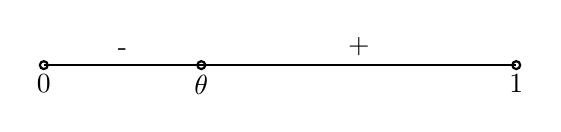
\begin{tikzpicture} [scale = 1] 
\draw[thick] (0.0, 0.0) -- (6.0, 0.0);
\draw[thick] (0.0, 0.0) circle [radius = 0.05];
\draw[thick] (2.0, 0.0) circle [radius = 0.05];
\draw[thick] (6.0, 0.0) circle [radius = 0.05];
\node[below] at (0.0, 0.0){$0$};
\node[below] at (2.0, 0.0){$\theta$};
\node[below] at (6.0, 0.0){$1$};
\node[above] at (1.0, 0.0){-};
\node[above] at (4.0, 0.0){+};
\end{tikzpicture} 
\end{figure}
\begin{align*}
P_{X} &= U\left[0, 1\right]
\end{align*}
\[ P\left(y = + | x\right) =\left\{ \begin{array}{ll}
1& \text{\;if\;} x \geq  \theta \\
0& \text{\;otherwise\;} \\
\end{array}\right. \]
\begin{align*}
&y  \in \left\{-, +\right\}
\end{align*}
\[ h_{a} =\left\{ \begin{array}{ll}
+& \text{\;if\;} x \geq  a \\
-& \text{\;otherwise\;} \\
\end{array}\right. \]
\begin{align*}
\mathcal{H} &= \left\{h_{a} : a \in \left[0, 1\right]\right\}
\\ &\ell: 0-1
\\ R\left(h_{a}\right)  &= | a - \theta |
\end{align*}
"wolves"
\newline \newline
\begin{figure}[H] \centering 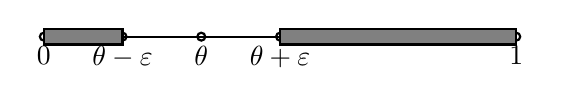
\begin{tikzpicture} [scale = 1] 
\draw[thick] (0.0, 0.0) -- (6.0, 0.0);
\draw[thick] (0.0, 0.0) circle [radius = 0.05];
\draw[thick] (2.0, 0.0) circle [radius = 0.05];
\draw[thick] (6.0, 0.0) circle [radius = 0.05];
\draw[thick] (1.0, 0.0) circle [radius = 0.05];
\draw[thick] (3.0, 0.0) circle [radius = 0.05];
\node[below] at (0.0, 0.0){$0$};
\node[below] at (2.0, 0.0){$\theta$};
\node[below] at (6.0, 0.0){$1$};
\node[below] at (1.0, 0.0){$\theta - \varepsilon$};
\node[below] at (3.0, 0.0){$\theta + \varepsilon$};
\draw[fill = gray, thick] (0.0, 0.1) rectangle (1.0, -0.1);
\draw[fill = gray, thick] (3.0, 0.1) rectangle (6.0, -0.1);
\end{tikzpicture} 
\end{figure}
S
\newline \newline
\begin{figure}[H] \centering 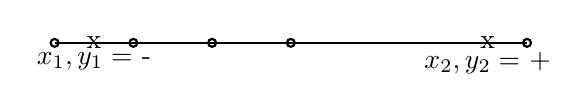
\begin{tikzpicture} [scale = 1] 
\draw[thick] (0.0, 0.0) -- (6.0, 0.0);
\draw[thick] (0.0, 0.0) circle [radius = 0.05];
\draw[thick] (2.0, 0.0) circle [radius = 0.05];
\draw[thick] (6.0, 0.0) circle [radius = 0.05];
\draw[thick] (1.0, 0.0) circle [radius = 0.05];
\draw[thick] (3.0, 0.0) circle [radius = 0.05];
\node[] at (0.5, 0.0){x};
\node[] at (5.5, 0.0){x};
\node[below] at (0.5, 0.0){$x_{1}, y_{1} =$ -};
\node[below] at (5.5, 0.0){$x_{2}, y_{2} =$ +};
\end{tikzpicture} 
\end{figure}
\begin{align*}
&  \mathbb{P} \left[\left\{S : \exists h \in \mathcal{H}_{\varepsilon}, \hat{R}\left(h\right) = 0\right\}\right]
\\ &= \mathbb{P} \left[\displaystyle\bigcup _{h \in \mathcal{H}_{\varepsilon}} \left\{S: \hat{R}\left(h\right) = 0\right\}\right]
\\ &\stackrel{Union b.}{\leq} \displaystyle\sum_{h \in \mathcal{H}_{\varepsilon}} \mathbb{P}\left[\left\{S: \hat{R}\left(h\right) = 0 \wedge R\left(h\right) > \varepsilon\right\}\right]
\\ &\stackrel{\mathcal{H}_{\varepsilon}}{\leq} \displaystyle\sum_{h \in \mathcal{H}_{\varepsilon}} \left(1 - \varepsilon\right)^{n}
\\ &\stackrel{\mathcal{H}_{\varepsilon} \subseteq \mathcal{H}}{\leq} \displaystyle\sum_{h \in \mathcal{H}} \left(1 - \varepsilon\right)^{n}
\\ &\stackrel{A3}{=} | \mathcal{H} | \left(1 - \varepsilon\right)^{n}
\\ &\stackrel{e^{-\varepsilon} \geq  1 - \varepsilon}{\leq} | \mathcal{H} | e^{-\varepsilon n} := \delta
\end{align*}
\begin{figure}[H] \centering \begin{tikzpicture} [scale = 1] 
\draw[thick] (1.0, 0.0) -- (1.0, 6.0);
\draw[thick] (0.0, 1.0) -- (6.0, 1.0);
\node[below right] at (6.0, 1.0){$\varepsilon$};
\draw[thick] (0.0, 5.0) -- (5.0, 0.0);
\node[left] at (0.0, 5.0){$1 - \varepsilon$};
\draw[thick] (0.0, 6.0)to [out = 280, in = 135](1.0, 4.0)to [out = 315, in = 170](5.0, 2.0);
\node[] at (3.0, 4.0){$e^{-\varepsilon} \geq  1 - \varepsilon$};
\end{tikzpicture} 
\end{figure}
\begin{align*}
- \varepsilon n &= \log\left(\dfrac{\delta}{| \mathcal{H} |}\right)
\\ \varepsilon &= \dfrac{1}{n} \log\left(\dfrac{| \mathcal{H} |}{\delta}\right)
\end{align*}
\begin{align*}
\mathbb{P}\left(\left\{\text{\;Bad\;} S\right\}\right) &\leq  \delta
\\ \mathbb{P}\left(\left(X \times Y\right)^{n} \setminus  \left\{\text{\;Bad\;} S\right\}\right) &> 1 - \delta
\\ \mathbb{P}\left[R\left(\hat{h}_{s}\right) \leq  \varepsilon\right] &\geq  1 - \delta
\end{align*}
With prob at least $1 - \delta$,
\begin{align*}
R\left(\hat{h}_{s}\right)  &\leq  \varepsilon := \dfrac{\log\left(| \mathcal{H} |\right) - \log\left(\delta\right)}{n}
\\ n  :&= \dfrac{\log\left(| \mathcal{H} |\right) - \log\left(\delta\right)}{\varepsilon}
\end{align*}



\section{Lecture $4$} 
A1: $\ell$ is $0-1$ loss
\begin{align*}
&\mathbb{P}_{S \sim  P^{n}}\left(\left\{S: \exists h \in \mathcal{H}_{\varepsilon}, \underbrace{\hat{R}_{s}\left(h\right) = 0}_{\text{\;A2: Realizable\;} \displaystyle\min_{h \in \mathcal{H}} R\left(h\right) = 0}\right\}\right)
\\ \mathcal{H}_{\varepsilon} &= \left\{h \in \mathcal{H} : R\left(h\right) > \varepsilon\right\}
\\ R\left(h\right)  &= \mathbb{E}_{\left(x, y\right) \sim  P} \ell\left(h\left(x\right), y\right)
\\ \hat{R}_{s}\left(h\right) &= \dfrac{1}{n} \displaystyle\sum_{x, y \in S} \ell\left(h\left(x\right), y\right)
\\ &  \mathbb{P}\left(\displaystyle\bigcup _{h \in \mathcal{H}_{\varepsilon}} \left\{S: \hat{R}_{s}\left(h\right) = 0\right\}\right)
\\ &\stackrel{\text{\;Union\;}}{\leq} \displaystyle\sum_{h \in \mathcal{H}_{\varepsilon}} \mathbb{P}\left(S: \hat{R}_{s}\left(h\right) = 0 \wedge R\left(h\right) > \varepsilon\right)
\\ &\stackrel{\text{\;Realizability\;}}{\leq} \displaystyle\sum_{h \in \mathcal{H}_{\varepsilon}} \left(1 - \varepsilon\right)^{n}
\\ &\stackrel{A3: | \mathcal{H} | < \infty}{\leq} | \mathcal{H} | \left(1 - \varepsilon\right)^{n}
\\ &\leq  | \mathcal{H} | e^{-\varepsilon n} := \delta
\end{align*}
\begin{align*}
n  &\geq  \dfrac{\log | \mathcal{H} | - \log \delta}{\varepsilon}
\\ \varepsilon &\leq  O\left(\dfrac{1}{n}\right) 
\end{align*}
Agnostic learning $\left(\text{\;wrt\;} \mathcal{H}\right), R\left(h^\star \right)  \geq  0$
\begin{align*}
&h^\star  \in \arg\displaystyle\min_{h \in \mathcal{H}} R\left(h\right) 
\end{align*}
e.g.
\begin{align*}
\mathbb{P}\left(y = +\right) &= \dfrac{1}{2}
\end{align*}
\begin{figure}[H] \centering 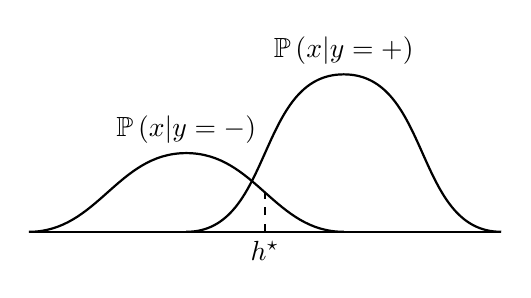
\begin{tikzpicture} [scale = 1] 
\draw[thick] (0.0, 0.0) -- (6.0, 0.0);
\draw[thick] (0.0, 0.0)to [out = 0, in = 180](2.0, 1.0)to [out = 0, in = 180](4.0, 0.0);
\draw[thick] (2.0, 0.0)to [out = 0, in = 180](4.0, 2.0)to [out = 0, in = 180](6.0, 0.0);
\node[above] at (2.0, 1.0){$\mathbb{P}\left(x | y = -\right)$};
\node[above] at (4.0, 2.0){$\mathbb{P}\left(x | y = +\right)$};
\node[below] at (3.0, 0.0){$h^\star $};
\draw[dashed, thick] (3.0, 0.0) -- (3.0, 0.5);
\end{tikzpicture} 
\end{figure}
Want Uniform Convergence:
\begin{align*}
&  \left\{S : \exists h \in \mathcal{H}, \left|  R\left(h\right) - \hat{R}_{s}\left(h\right)  \right| > \varepsilon\right\}
\\ &  \;\forall\; h \in \mathcal{H}, | R\left(h\right) - \hat{R}_{s}\left(h\right) | \leq  \varepsilon
\end{align*}
" $R\left(\hat{h}_{s}\right)  - R\left(h^\star \right)$ small"
\newline \newline
\begin{align*}
&  \mathbb{P}\left(\left\{S : \exists h \in \mathcal{H}, \left|  R\left(h\right) - \hat{R}_{s}\left(h\right)  \right| > \varepsilon\right\}\right)
\\ &\leq  \displaystyle\sum_{h \in \mathcal{H}} \mathbb{P}\left(\left\{S : \left|  R\left(h\right) - \hat{R}_{s}\left(h\right)  \right| > \varepsilon\right\}\right)
\\ &\stackrel{\text{\;Hoeffding's\;}}{\leq} 2 | \mathcal{H} | e^{- \dfrac{2 n \varepsilon^{2}}{\left(b - a\right)^{2}}} := \delta
\end{align*}
new A1: $\ell \in \left[a , b \right]$ or $_{\left(x, y\right) \sim  P} \ell\left(h\left(x\right), y\right)$ is subGaussian
\\* remove A2
\\* retain A3
\\* Hoeffding's Ineq. $\left|  \mu - \dfrac{1}{n} \displaystyle\sum_{i}^{n} \theta_{i}  \right|$
\begin{align*}
&  \mathbb{P}_{S \sim  P^{n}}\left(\left\{S: \left|  R\left(h\right) - \hat{R}_{s}\left(h\right)  \right| > \varepsilon\right\}\right) \leq  2 e^{- \dfrac{2 n \varepsilon^{2}}{\left(b - a\right)^{2}}}
\\ &  \boxed{\text{\;wp\;} \geq  1 - \delta, \;\forall\; h \in \mathcal{H}, \left|  R\left(h\right) - \hat{R}_{s}\left(h\right)  \right| \leq  \varepsilon}
\end{align*}
\begin{align*}
&  R\left(\hat{h}_{s}\right) - R\left(h^\star \right)
\\ &= R\left(\hat{h}_{s}\right) - \hat{R}_{s}\left(\hat{h}_{s}\right) + \hat{R}_{s}\left(\hat{h}_{s}\right) - \hat{R}_{s}\left(h^\star \right) + \hat{R}_{s}\left(h^\star \right) - R\left(h^\star \right)
\\ &\leq  \varepsilon + \underbrace{\left(\hat{R}_{s}\left(\hat{h}_{s}\right) - \hat{R}_{s}\left(h^\star \right)\right)}_{\text{\;ERM\;} \leq  0} + \varepsilon
\\ &\leq  2 \varepsilon
\end{align*}
\begin{align*}
\dfrac{2 n \varepsilon^{2}}{\left(b - a\right)^{2}} &=  \log \dfrac{2 | \mathcal{H} |}{\delta}
\\ n  &= \dfrac{\log \left(2 | \mathcal{H} |\right) - \log \delta}{2 \varepsilon^{2}} \left(b - a\right)^{2}
\\ \varepsilon &\leq  O\left(\dfrac{1}{\sqrt{n}}\right) 
\end{align*}
"learning alg" $A\left(S\right)  = h $
\newline \newline



\section{Lecture $5$} 
\begin{align*}
\mathbb{P}\left(\left\{S  \text{\;bad\;}\right\}\right) &\leq  \delta = | \mathcal{H} | e^{-n \varepsilon}
\end{align*}
i.e. $\exists h, \left|  R\left(h\right) - \hat{R}_{s}\left(h\right)  \right| > \varepsilon$
\\* Today's goal: $\mathbb{P}\left(\left\{S  \text{\;bad\;}\right\}\right) \geq  \delta$
\newline \newline
Any learning Algorithm $A  : \left\{S\right\} \to  \mathcal{H}$, ERM is a $A $
\begin{align*}
S  &\stackrel{iid}{\sim} P^{n}\left(x, y\right), n \leq  \dfrac{| X |}{2}
\end{align*}
\begin{thm} \label{thm:bad} 
$\;\forall\; A, \exists P$
\end{thm}
\begin{enumerate}
\item $\exists h : X \to  Y, R_{P}\left(h\right) = 0$
\item $\mathbb{P}\left(\left\{S: R_{P}\left(A\left(S\right)\right) \geq  \dfrac{1}{8}\right\}\right) \geq  \dfrac{1}{7}$
\end{enumerate}

\begin{align*}
2 n &= \left| \left\{\text{\;distinct\;} x's \text{\;in\;} S\right\} \cup \left\{\text{\;some other distinct\;} x \text{\;from\;} X \text{\;not in\;} S\right\} \right|
\\ &\overbrace{x_{1}, ..., x_{n}}^{S_{n}}, x_{n+1}, ..., x_{2n}
\end{align*}
Construct a family of $P\left(x, y\right)  = P\left(x\right) \cdot  P\left(y | x\right)$
\begin{enumerate}
\item $P\left(x\right) $ uniform on the $2 n$ items
\item $\mathcal{C} := 2^{2n}$ labelings over $2 n$ items
\end{enumerate}

\[ \mathcal{C} \text{\;rows\;} \Rightarrow  \mathcal{C} \text{\;joint\;} P_{XY} =\left\{ \begin{array}{ll}
0 ... 0 ... 0 ... 0 0, \mathbb{P}\left(y = 1 | x\right) = 0 \;\forall\; x  & \\
0 ... 0 ... 0 ... 0 1, \mathbb{P}\left(y = 1 | x_{2n}\right) = 1, \mathbb{P}\left(y = 1 | x \neq  x_{2n}\right) = 0 & \\
1 ... 1 ... 1 ... 1 1, \mathbb{P}\left(y = 1 | x\right) = 1 \;\forall\; x  & \\
\end{array}\right. \]
Key idea: $\displaystyle\max_{c \in \left[\mathcal{C}\right]} \mathbb{E}_{S \sim  P^{n}_{c}} R_{P_{c}}\left(A\left(S\right)\right)$
\begin{align*}
&\boxed{z \text{\;rv\;} \geq  0, \mathbb{E}\left(z\right) \geq  a \Rightarrow  \mathbb{P}\left(z \geq  b\right) \geq  c}
\\ &\boxed{z \in \left[0, 1\right] \text{\;rv\;}, \mathbb{E}\left(z\right) \geq  u \Rightarrow  \mathbb{P}\left(z \geq  1 - a\right) \geq  \dfrac{u - \left(1 - a\right)}{a}}
\end{align*}
Lemma B.$1$ Markov's ineq
\newline \newline
$Q  = \left(2 n\right)^{n}$ distinct $S $ sequences, $S_{1}, S_{2}, ..., S_{Q}$
\newline \newline



\section{Lecture $6$} 
Take $2 n$ distinct item from $X $
\begin{align*}
&x_{1} ... x_{2n}
\\ &0 ... 00
\\ &0 ... 01
\\ &...
\end{align*}
$\mathcal{C} := 2^{2n}$ different labelings of the $2 n$ items
\begin{align*}
&  P_{1}\left(y | x\right) \text{\;"world"\;} P_{1}\left(x, y\right) = P\left(x\right) P_{1}\left(y | x\right)
\\ &...
\\ &P_{\mathcal{C}}\left(y | x\right)
\\ P\left(x\right)  &= \dfrac{1}{2n}
\\ R_{c}\left(h\right) &= \mathbb{E}_{\left(x, y\right) \sim  P_{c}\left(x, y\right)} \underbrace{\ell}_{0-1 \text{\;loss\;}} \left(h\left(x\right), y\right), c \in \left[\mathcal{C}\right]
\end{align*}
\begin{align*}
n  &\leq  \dfrac{| X |}{2}
\end{align*}
No-Free lunch Thm
\begin{align*}
&\;\forall\; A, \exists P_{c} \left(c \in \left[\mathcal{C}\right]\right)
\end{align*}
\begin{enumerate}
\item $\exists h, R_{c}\left(h\right) = 0$
\item $\mathbb{P}_{S \sim  P_{c}^{n}} \left[R_{c}\left(A\left(S\right)\right) \geq  \dfrac{1}{8} \right] \geq  \dfrac{1}{7}$
\end{enumerate}

\begin{align*}
\displaystyle\max_{c \sim  \left[\mathcal{C}\right]} \mathbb{E}_{S \sim  P^{n}} R_{c}\left(A\left(S\right)\right) &\geq  \dfrac{1}{4} \stackrel{\text{\;Markov\;}}{\Rightarrow} \left(2\right)
\\ S  &= \left(x^{1}, x^{2}, ..., x^{n}\right), x^{i \leftarrow \text{\;position in\;} S}
\\ &S_{1}: x_{1}, x_{1}, ..., x_{1}
\\ &S_{2}: x_{1}, ..., x_{1}, x_{2}
\\ &...
\\ &S_{Q}: x_{2n}, ..., x_{2n}
\\ Q  :&= \left(2 n\right)^{n}
\end{align*}
\begin{align*}
&  \displaystyle\max_{c \in \left[\mathcal{C}\right]} \mathbb{E}_{S \sim  P_{c}^{n}} R_{c}\left(A\left(S\right)\right)
\\ &= \displaystyle\max_{c \in \left[\mathcal{C}\right]} \dfrac{1}{Q} \displaystyle\sum_{q=1}^{Q} R_{c}\left(A\left(S_{q}\right)\right)
\\ &\geq  \dfrac{1}{\mathcal{C}} \displaystyle\sum_{c=1}^{\mathcal{C}} \dfrac{1}{Q} \displaystyle\sum_{q=1}^{Q} R_{c}\left(A\left(S_{q}\right)\right)
\\ &= \dfrac{1}{Q} \displaystyle\sum_{q=1}^{Q} \dfrac{1}{\mathcal{C}} \displaystyle\sum_{c=1}^{\mathcal{C}} R_{c}\left(A\left(S_{q}\right)\right)
\\ &\stackrel{P_{x} \text{\;Unif\;}}{=} \dfrac{1}{Q} \displaystyle\sum_{q=1}^{Q} \dfrac{1}{\mathcal{C}} \displaystyle\sum_{c=1}^{\mathcal{C}} \dfrac{1}{2n} \displaystyle\sum_{i=1}^{2n} \mathbbm{1}_{\left[A\left(S_{q}\right)\left(x_{i}\right) \neq  y_{c}\left(x_{i}\right)\right]}
\end{align*}
\begin{align*}
t  :&= \left|  \left\{x_{1}, ..., x_{2n}\right\} \setminus  \left\{S_{q}\right\}  \right| \geq  n 
\end{align*}
Let $\left\{v_{1}, ..., v_{t}\right\}$ be the set
\newline \newline
\begin{align*}
&\stackrel{\text{\;only consider\;} \left\{v \right\}}{\geq} \dfrac{1}{Q} \displaystyle\sum_{q=1}^{Q} \dfrac{1}{\mathcal{C}} \displaystyle\sum_{c=1}^{\mathcal{C}} \dfrac{1}{2n} \displaystyle\sum_{i=1}^{t} \mathbbm{1}_{\left[A\left(S_{q}\right)\left(v_{i}\right) \neq  y_{c}\left(v_{i}\right)\right]}
\\ &= \dfrac{1}{Q} \displaystyle\sum_{q=1}^{Q} \dfrac{1}{2n} \displaystyle\sum_{i=1}^{t} \underbrace{ \dfrac{1}{\mathcal{C}} \displaystyle\sum_{c=1}^{\mathcal{C}} \mathbbm{1}_{\left[A\left(S_{q}\right)\left(v_{i}\right) \neq  y_{c}\left(v_{i}\right)\right]} }_{\dfrac{1}{2}}
\\ &= \dfrac{1}{Q} \displaystyle\sum_{q=1}^{Q} \dfrac{1}{2n} \displaystyle\sum_{i=1}^{t} \dfrac{1}{2}
\\ &= \dfrac{1}{Q} \displaystyle\sum_{q=1}^{Q} \dfrac{1}{2n} \dfrac{1}{2} t
\\ &\geq  \dfrac{1}{2} \displaystyle\sum_{q=1}^{Q} \dfrac{1}{2n} \dfrac{1}{2} n
\\ &= \dfrac{1}{4}
\end{align*}
\[ h_{c}\left(x\right) =\left\{ \begin{array}{ll}
0& \text{\;if\;} x \notin \mathbb{Z} \\
y_{c}\left(x\right)& \text{\;otherwise\;} \\
\end{array}\right. \]
\begin{align*}
| \mathcal{H} | &= \infty
\end{align*}
ex $6.1$
\begin{align*}
\mathcal{H} &= \left\{h_{A} : a \in \mathbb{R}\right\}
\end{align*}
\begin{figure}[H] \centering 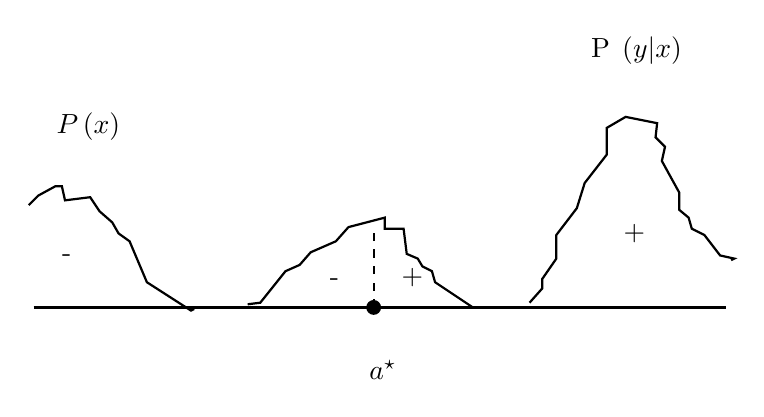
\begin{tikzpicture} [scale = 1] 
\node[right] at (7.66, 5.26){$\text{\;P\;}\left(y | x\right)$};
\node[right] at (0.97, 4.3){$P\left(x\right) $};
\node[right] at (8.17, 2.94){+};
\node[right] at (4.44, 2.36){-};
\node[right] at (5.35, 2.38){+};
\node[right] at (1.04, 2.66){-};
\draw[black, thick] (7.1, 2.06) -- (7.26, 2.24) -- (7.26, 2.36) -- (7.44, 2.62) -- (7.44, 2.92) -- (7.7, 3.26) -- (7.8, 3.58) -- (8.08, 3.94) -- (8.08, 4.28) -- (8.32, 4.42) -- (8.72, 4.34) -- (8.7, 4.16) -- (8.82, 4.04) -- (8.78, 3.86) -- (9.0, 3.46) -- (9.0, 3.24) -- (9.12, 3.14) -- (9.16, 3.0) -- (9.32, 2.92) -- (9.52, 2.66) -- (9.7, 2.62) -- (9.66, 2.6);
\draw[black, thick] (3.52, 2.04) -- (3.68, 2.06) -- (4.0, 2.46) -- (4.18, 2.54) -- (4.32, 2.7) -- (4.64, 2.84) -- (4.8, 3.02) -- (5.26, 3.14) -- (5.26, 3.0) -- (5.5, 3.0) -- (5.54, 2.68) -- (5.68, 2.62) -- (5.74, 2.52) -- (5.86, 2.46) -- (5.9, 2.32) -- (6.38, 2.0);
\draw[black, thick] (0.74, 3.3) -- (0.86, 3.42) -- (1.08, 3.54) -- (1.16, 3.54) -- (1.2, 3.36) -- (1.52, 3.4) -- (1.64, 3.22) -- (1.8, 3.08) -- (1.88, 2.94) -- (2.02, 2.84) -- (2.24, 2.32) -- (2.8, 1.96) -- (2.84, 1.98);
\node[right] at (4.94, 1.2){$a^\star $};
\draw[black, fill = black, thick] (5.12, 2.0) ellipse (0.08 and 0.08);
\draw[black, dashed, thick] (5.12, 2.0) -- (5.12, 3.0);
\draw[black, thick] (0.8, 2.0) -- (9.6, 2.0);
\end{tikzpicture} 
\end{figure}
\[ h_{a}\left(x\right) =\left\{ \begin{array}{ll}
1& \text{\;if\;} x \geq  a \\
0& \text{\;otherwise\;} \\
\end{array}\right. \]
\begin{figure}[H] \centering 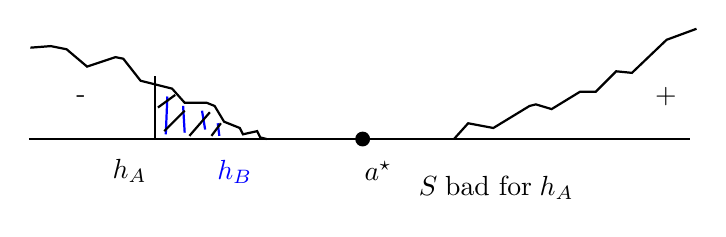
\begin{tikzpicture} [scale = 1] 
\draw[blue, thick] (3.2, 1.8) -- (3.22, 1.64);
\draw[blue, thick] (3.0, 1.96) -- (3.04, 1.72);
\draw[blue, thick] (2.76, 2.02) -- (2.78, 1.68);
\draw[blue, thick] (2.56, 2.14) -- (2.54, 1.66);
\draw[black, thick] (3.24, 1.8) -- (3.12, 1.64);
\draw[black, thick] (2.78, 1.96) -- (2.52, 1.7);
\draw[black, thick] (3.1, 1.94) -- (2.84, 1.64);
\draw[black, thick] (2.66, 2.16) -- (2.44, 2.0);
\draw[black, thick] (2.4, 2.4) -- (2.4, 1.6);
\node[blue, right] at (3.07, 1.18){$h_{B}$};
\node[right] at (5.63, 0.98){$S  \text{\;bad for\;} h_{A}$};
\node[right] at (8.63, 2.14){+};
\node[right] at (1.28, 2.14){-};
\draw[black, thick] (6.2, 1.6) -- (6.38, 1.8) -- (6.7, 1.74) -- (7.16, 2.02) -- (7.24, 2.04) -- (7.44, 1.98) -- (7.8, 2.2) -- (8.0, 2.2) -- (8.26, 2.46) -- (8.46, 2.44) -- (8.9, 2.86) -- (9.28, 3.0);
\draw[black, thick] (0.82, 2.76) -- (1.08, 2.78) -- (1.28, 2.74) -- (1.54, 2.52) -- (1.9, 2.64) -- (2.0, 2.62) -- (2.22, 2.34) -- (2.62, 2.24) -- (2.78, 2.06) -- (3.06, 2.06) -- (3.16, 2.02) -- (3.28, 1.82) -- (3.48, 1.74) -- (3.52, 1.66) -- (3.7, 1.7) -- (3.74, 1.62) -- (3.82, 1.6);
\node[right] at (1.74, 1.2){$h_{A}$};
\node[right] at (4.94, 1.2){$a^\star $};
\draw[black, fill = black, thick] (5.04, 1.6) ellipse (0.08 and 0.08);
\draw[black, thick] (0.8, 1.6) -- (9.2, 1.6);
\end{tikzpicture} 
\end{figure}
\begin{align*}
\mathbb{P}\left(\displaystyle\bigcup _{h \in \mathcal{H}_{\varepsilon}} \left\{S \text{\;makes\;} h, 0 \text{\;training risk\;}\right\}\right) &\leq  \displaystyle\sum_{h \in \mathcal{H}_{\varepsilon}} \mathbb{P}\left(\left\{S_{\text{\;bad\;}}\right\}\right)
\end{align*}
\begin{figure}[H] \centering 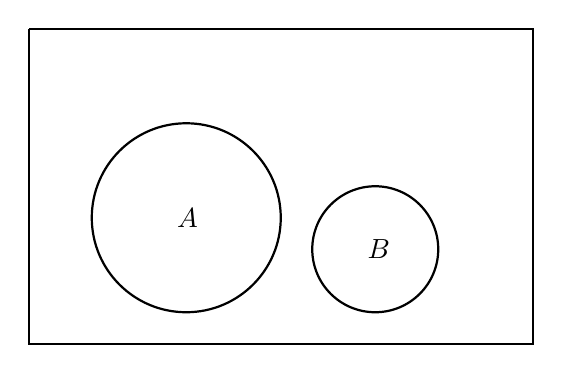
\begin{tikzpicture} [scale = 1] 
\node[right] at (5.78, 4.0){$B $};
\node[right] at (3.36, 4.4){$A $};
\draw[black, thick] (6.0, 4.0) ellipse (0.8 and 0.8);
\draw[black, thick] (3.6, 4.4) ellipse (1.2 and 1.2);
\draw[black, thick] (1.6, 6.8) -- (1.6, 2.8) -- (8.0, 2.8) -- (8.0, 4.4) -- (8.0, 6.8) -- (1.6, 6.8);
\end{tikzpicture} 
\end{figure}
\begin{figure}[H] \centering 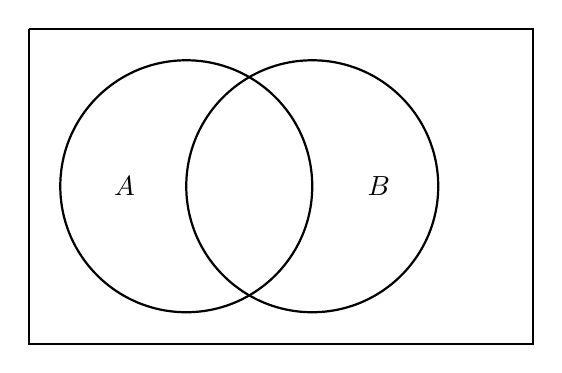
\begin{tikzpicture} [scale = 1] 
\node[right] at (5.78, 4.8){$B $};
\node[right] at (2.56, 4.8){$A $};
\draw[black, thick] (5.2, 4.8) ellipse (1.6 and 1.6);
\draw[black, thick] (3.6, 4.8) ellipse (1.6 and 1.6);
\draw[black, thick] (1.6, 6.8) -- (1.6, 2.8) -- (8.0, 2.8) -- (8.0, 4.4) -- (8.0, 6.8) -- (1.6, 6.8);
\end{tikzpicture} 
\end{figure}
\begin{align*}
P\left(A \text{\;or\;} B\right)  &\leq  P\left(A\right)  + P\left(B\right) 
\end{align*}



\section{Lecture $7$} 
Recall: finite $\mathcal{H}$
\begin{align*}
\mathbb{P}_{S \sim  P^{n}} &  \left(\displaystyle\max_{h \in \mathcal{H}} R\left(h\right) - \hat{R}_{s}\left(h\right) \leq  \varepsilon\right) \geq  1 - \delta
\\ \varepsilon &= \sqrt{\dfrac{\log | \mathcal{H} | + \log \dfrac{1}{\delta}}{2n}}
\end{align*}
Today: Any $\mathcal{H} = \left\{h \right\}, h: X \to  Y $
\\* ex. $\mathcal{H} = \left\{\underbrace{h_{a}\left(x\right)}_{a \in \mathbb{R}} = \text{sign}\left[\sin\left(a x\right)\right]\right\}$
\begin{align*}
VC  &= \infty
\end{align*}
Growth number
\begin{align*}
G\left(n\right)  :&= \displaystyle\sup_{x_{1}, ..., x_{n} \in X} \left|  \left\{\mathbbm{1}_{\left[h\left(x1\right) \neq  y_{1}\right]}, ..., \mathbbm{1}_{\left[h\left(x_{n}\right) \neq  y_{n}\right]} : h \in \mathcal{H}\right\}  \right|
\\ &\left(y_{i} = h^\star \left(x_{i}\right)\right)
\\ d  :&= VC\left(\mathcal{H}\right)  = \arg\displaystyle\max_{n} G_{\mathcal{H}}\left(n\right) = 2^{n}
\end{align*}
ex: $\mathcal{H} = \left\{\underbrace{h_{a}\left(x\right)}_{X = \mathbb{R}} = \left\{1, x \geq  a, 0 \text{\;ow\;}\right\}, a \in \mathbb{R}\right\}$
\newline \newline
\begin{figure}[H] \centering 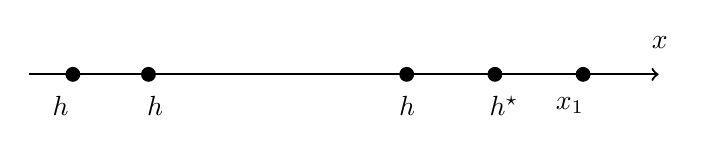
\begin{tikzpicture} [scale = 1] 
\node[black, right] at (8.99, 3.2){$x $};
\node[black, right] at (7.77, 2.4){$x_{1}$};
\node[black, right] at (6.93, 2.4){$h^\star $};
\node[black, right] at (5.78, 2.4){$h $};
\node[black, right] at (2.58, 2.4){$h $};
\node[black, right] at (1.38, 2.4){$h $};
\draw[black, fill = black, thick] (8.24, 2.8) ellipse (0.08 and 0.08);
\draw[black, fill = black, thick] (7.12, 2.8) ellipse (0.08 and 0.08);
\draw[black, fill = black, thick] (6.0, 2.8) ellipse (0.08 and 0.08);
\draw[black, fill = black, thick] (2.72, 2.8) ellipse (0.08 and 0.08);
\draw[black, fill = black, thick] (1.76, 2.8) ellipse (0.08 and 0.08);
\draw[->, black, thick] (1.2, 2.8) -- (9.2, 2.8);
\end{tikzpicture} 
\end{figure}
\begin{align*}
&  \left(\mathbbm{1}_{\left[h\left(x_{1}\right) \neq  0\right]}\right)
\\ &  \left|  \left\{\left(0\right), \left(1\right)\right\}  \right| = 2
\end{align*}
\begin{align*}
G\left(1\right)  &= 2, VC\left(\mathcal{H}\right)  = 1
\\ G\left(2\right)  &= 3
\\ &G\left(3\right) 
\end{align*}
\begin{figure}[H] \centering 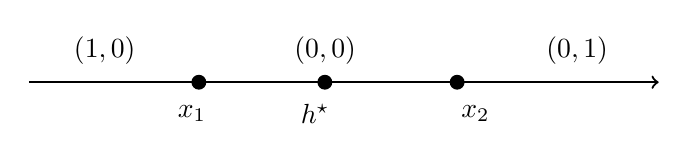
\begin{tikzpicture} [scale = 1] 
\node[black, right] at (7.65, 4.0){$\left(0, 1\right)$};
\node[black, right] at (4.45, 4.0){$\left(0, 0\right)$};
\node[black, right] at (1.65, 4.0){$\left(1, 0\right)$};
\node[black, right] at (6.57, 3.2){$x_{2}$};
\node[black, right] at (4.53, 3.2){$h^\star $};
\node[black, right] at (2.97, 3.2){$x_{1}$};
\draw[black, fill = black, thick] (6.64, 3.6) ellipse (0.08 and 0.08);
\draw[black, fill = black, thick] (4.96, 3.6) ellipse (0.08 and 0.08);
\draw[black, fill = black, thick] (3.36, 3.6) ellipse (0.08 and 0.08);
\draw[->, black, thick] (1.2, 3.6) -- (9.2, 3.6);
\end{tikzpicture} 
\end{figure}
\begin{figure}[H] \centering 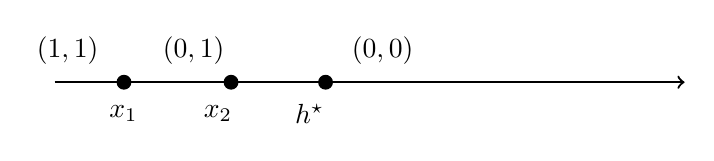
\begin{tikzpicture} [scale = 1] 
\node[black, right] at (4.85, 2.8){$\left(0, 0\right)$};
\node[black, right] at (2.45, 2.8){$\left(0, 1\right)$};
\node[black, right] at (0.85, 2.8){$\left(1, 1\right)$};
\node[black, right] at (4.13, 2.0){$h^\star $};
\node[black, right] at (2.97, 2.0){$x_{2}$};
\node[black, right] at (1.77, 2.0){$x_{1}$};
\draw[black, fill = black, thick] (4.64, 2.4) ellipse (0.08 and 0.08);
\draw[black, fill = black, thick] (3.44, 2.4) ellipse (0.08 and 0.08);
\draw[black, fill = black, thick] (2.08, 2.4) ellipse (0.08 and 0.08);
\draw[->, black, thick] (1.2, 2.4) -- (9.2, 2.4);
\end{tikzpicture} 
\end{figure}
\begin{figure}[H] \centering 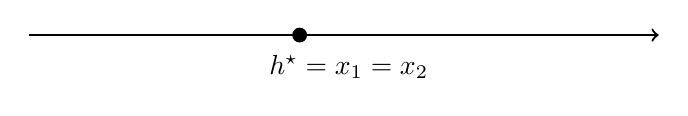
\begin{tikzpicture} [scale = 1] 
\node[black, right] at (4.13, 2.0){$h^\star  = x_{1} = x_{2}$};
\draw[black, fill = black, thick] (4.64, 2.4) ellipse (0.08 and 0.08);
\draw[->, black, thick] (1.2, 2.4) -- (9.2, 2.4);
\end{tikzpicture} 
\end{figure}
\begin{figure}[H] \centering \begin{tikzpicture} [scale = 1] 
\node[black, right] at (4.12, 1.2){$VC\left(\mathcal{H}\right) $};
\node[black, right] at (8.58, 1.6){$n $};
\node[black, right] at (1.17, 8.0){$G\left(n\right) $};
\draw[black, dashed, thick] (4.8, 4.8) -- (4.8, 1.6);
\draw[black, thick] (4.8, 4.8).. controls(6.26, 5.06)and(7.46, 5.86)..(8.4, 7.2);
\draw[black, thick] (1.6, 1.6).. controls(3.19, 2.66)and(4.26, 3.73)..(4.8, 4.8);
\draw[<->, black, thick] (1.6, 7.6) -- (1.6, 1.6) -- (8.4, 1.6);
\end{tikzpicture} 
\end{figure}
Proof outline
\begin{itemize}
\item Introduce "ghost sample" $S' \sim  P^{n}$
\end{itemize}\begin{align*}
\hat{R}'_{s'}\left(h\right) &= \dfrac{1}{n} \displaystyle\sum_{x', y' \in S'} \ell\left(h\left(x'\right), y'\right)
\end{align*}
\begin{itemize}
\item Symmertrization Lemma
\end{itemize}\begin{align*}
\boxed{\;\forall\; \varepsilon \geq  \sqrt{\dfrac{2 \log 2}{n}}}, \mathbb{P}_{s \sim  P^{n}}\left(\displaystyle\sup_{h \in \mathcal{H}} R\left(h\right) - \hat{R}_{s}\left(h\right) > \varepsilon\right) &\stackrel{\text{\;Sym lemma\;}}{\leq} 2 \mathbb{P}_{s}\left(\displaystyle\sup_{h \in \mathcal{H}} \hat{R}'_{s'}\left(h\right) - \hat{R}_{s}\left(h\right) > \dfrac{\varepsilon}{2}\right)
\end{align*}
define
\begin{align*}
&\boxed{ \left\{\left(\underbrace{\ell\left(h\left(x_{1}\right), y_{1}\right), ..., \ell\left(h\left(x_{n}\right), y_{n}\right)}_{S }, \underbrace{\ell\left(h\left(x'_{1}\right), y'_{1}\right), ... \ell\left(h\left(x'_{n}\right), y'_{n}\right)}_{S'}\right) : h \in \mathcal{H}\right\} := Vec\left(2 n\right)  }
\\ &\stackrel{\text{\;def\;} Vec\left(2 n\right) }{=} 2 \mathbb{P}_{s} \left(\displaystyle\max_{h \in Vec\left(2n\right) } \hat{R}'_{s'}\left(h\right) - \hat{R}_{s}\left(h\right) > \dfrac{\varepsilon}{2}\right)
\\ &\stackrel{\text{\;Union b\;}}{\leq} 2 | Vec\left(2 n\right)  | \mathbb{P}\left(\hat{R}'_{s'}\left(h\right) - \hat{R}_{s}\left(h\right) > \dfrac{\varepsilon}{2}\right)
\\ &\stackrel{\text{\;Growth num\;}}{\leq} 2 G_{\mathcal{H}}\left(2 n \right) \mathbb{P}\left(\hat{R}'_{s'}\left(h\right) - \hat{R}_{s}\left(h\right) > \dfrac{\varepsilon}{2}\right)
\\ &\stackrel{\text{\;Hoeffding's\;} \left(2 \text{\;samples\;}\right)}{\leq} 2 G_{\mathcal{H}}\left(2 n \right) e^{- \dfrac{n \left(\dfrac{\varepsilon}{2}\right)^{2}}{2}}
\\ &\stackrel{\varepsilon \geq  \sqrt{\dfrac{2 \log 2}{n}}}{\Rightarrow} \text{\;wp\;} \geq  1 - \delta, \displaystyle\sup_{h \in \mathcal{H}} R\left(h\right) - \hat{R}_{s}\left(h\right) \leq  2 \sqrt{2 \dfrac{\log G_{\mathcal{H}}\left(2 n \right) + \log \dfrac{2}{\delta}}{n}}
\end{align*}
"Tighter than VC-bound"
\newline \newline



\section{Lecture $8$} 
Growth number $G_{\mathcal{H}}\left(n\right) := \displaystyle\sup_{x_{1} ... x_{n} \in X} \left|  \left\{\left(h\left(x_{1}\right), ..., h\left(x_{n}\right)\right) : h \in \mathcal{H}\right\}  \right|$
\\* symmetrization lemma
\begin{align*}
&\;\forall\; \underbrace{\boxed{\varepsilon \geq  \sqrt{\dfrac{2 \log 2}{n}}}}_{\text{\;Assumption A1\;}},
\\ &  P\left(\displaystyle\sup_{h \in \mathcal{H}} R\left(h\right) - \hat{R}\left(h\right) > \varepsilon\right) \leq  2 P\left(\displaystyle\sup_{h \in \mathcal{H}} \underbrace{\hat{R}'\left(h\right)}_{\text{\;ghost sample\;}} - \hat{R}\left(h\right) > \dfrac{\varepsilon}{2}\right)
\\ &\Rightarrow  P\left(\displaystyle\sup_{h \in \mathcal{H}} R\left(h\right) - \hat{R}\left(h\right) > \varepsilon\right) \leq  2 G_{\mathcal{H}}\left(2 n \right) e^{- \dfrac{n \left(\dfrac{\varepsilon}{2}\right)^{2}}{2}} := \delta
\\ \varepsilon :&= \sqrt{\dfrac{8 \left(\log 2 G_{\mathcal{H}}\left(2 n\right) - \log \delta\right)}{n}}
\end{align*}
VC-dim of $\mathcal{H} := d $
\begin{align*}
d  &= \displaystyle\max_{n} n : G_{\mathcal{H}}\left(n\right) = 2^{n}
\end{align*}
Sawer's Lemma:
\\* Assuming $d  < \infty$. Then
\begin{align*}
G_{n}\left(n\right) &\leq  \displaystyle\sum_{i=0}^{d} \dbinom{n}{i}
\\ &\Rightarrow  \text{\;If\;} n  \geq  d, G_{\mathcal{H}}\left(n\right) \leq  \left(\dfrac{e n}{d}\right)^{d}
\\ &  P\left(\displaystyle\sup_{h \in \mathcal{H}} R\left(h\right) - \hat{R}\left(h\right) > \varepsilon\right)  \leq  2 \left(\dfrac{2 e n}{d}\right)^{d} e^{- \dfrac{n \varepsilon^{2}}{8}} := \delta
\\ &\Rightarrow  \varepsilon = \sqrt{8 \dfrac{d \log n + d \log \dfrac{2 e}{d} + \log \dfrac{2}{\delta}}{n}} \Rightarrow  O\left(\sqrt{ \dfrac{d}{n}}\right)
\end{align*}
Proof of Sym Lemma. Let a "worst" hypo be $h_{w} \in \arg\displaystyle\sup_{h \in \mathcal{H}} R\left(h\right) - \hat{R}\left(h\right)$
\begin{align*}
&  \mathbbm{1}_{\left[R\left(h_{w}\right) - \hat{R}\left(h_{w}\right) > \varepsilon\right]} \cdot  \mathbbm{1}_{\left[R\left(h_{w}\right) - \underbrace{\hat{R}'\left(h_{w}\right)}_{\text{\;ghost\;}} < \dfrac{\varepsilon}{2}\right]}
\\ &= \mathbbm{1}_{\left[R\left(h_{w}\right) - \hat{R}\left(h_{w}\right) > \varepsilon \wedge \left(\hat{R}'\left(h_{w}\right) - R\left(h_{w}\right)\right) > - \dfrac{\varepsilon}{2}\right]}
\end{align*}
\begin{figure}[H] \centering 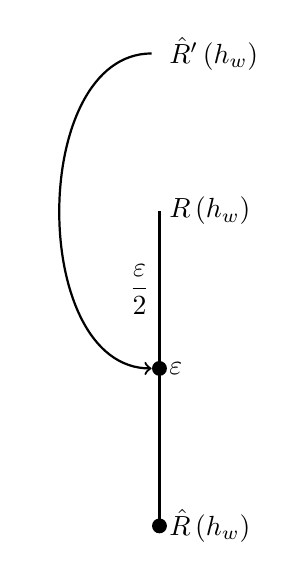
\begin{tikzpicture} [scale = 1] 
\draw[thick] (0.0, 0.0) -- (0.0, 4.0);
\draw[fill = black, thick] (0.0, 0.0) circle [radius = 0.08];
\draw[fill = black, thick] (0.0, 2.0) circle [radius = 0.08];
\node[right] at (0.0, 0.0){$\hat{R}\left(h_{w}\right)$};
\node[right] at (0.0, 2.0){$\varepsilon$};
\node[right] at (0.0, 4.0){$R\left(h_{w}\right) $};
\node[right] at (0.0, 6.0){$\hat{R}'\left(h_{w}\right)$};
\node[left] at (0.0, 3.0){$\dfrac{\varepsilon}{2}$};
\draw[->, thick] (-0.1, 6.0)to [out = 180, in = 180](-0.1, 2.0);
\end{tikzpicture} 
\end{figure}
\begin{align*}
&\stackrel{\text{\;implication\;}}{\leq} \mathbbm{1}_{\left[\hat{R}'\left(h_{w}\right) - \hat{R}\left(h_{w}\right) > \dfrac{\varepsilon}{2}\right]}
\\ &\stackrel{\text{\;expectation over ghost sample\;} S'}{\Rightarrow} \mathbbm{1}_{\left[R\left(h_{w}\right) - \hat{R}\left(h_{w}\right) > \varepsilon\right]} \underbrace{P'}_{\text{\;wrt\;} S' \sim  P^{n}_{X Y}} \left(R\left(h_{w}\right) - \hat{R}'\left(h_{w}\right) < \dfrac{\varepsilon}{2}\right)
\\ &\leq  P'\left(\hat{R}'\left(h_{w}\right) - \hat{R}\left(h_{w}\right) > \dfrac{\varepsilon}{2}\right) \to  \boxed{1}
\end{align*}
By Hoeffding's Ineq
\begin{align*}
&  P'\left(R\left(h_{w}\right) - \hat{R}'\left(h_{w}\right) < \dfrac{\varepsilon}{2}\right) \geq  1 - e^{- 2 n \left(\dfrac{\varepsilon}{2}\right)^{2}} \stackrel{\text{\;A1\;}}{\geq} \dfrac{1}{2}
\\ \boxed{1} &\Rightarrow  \mathbbm{1}_{\left[R\left(h_{w}\right) - \hat{R}\left(h_{w}\right) > \varepsilon\right]} \leq  2 P'\left(\hat{R}'\left(h_{w}\right) - \hat{R}\left(h_{w}\right) > \dfrac{\varepsilon}{2}\right)
\\ &\stackrel{h_{w} \text{\;def\;}}{\Rightarrow} \mathbbm{1}_{\left[\displaystyle\sup_{h \in \mathcal{H}} R\left(h\right) - \hat{R}\left(h\right) > \varepsilon\right]} \leq  \text{\;RHS above\;} \stackrel{\text{\;implication\;}}{\leq} 2 P'\left(\displaystyle\sup_{h \in \mathcal{H}} \hat{R}'\left(h\right) - \hat{R}\left(h\right) > \dfrac{\varepsilon}{2}\right)
\\ &\stackrel{\text{\;sym\;} S  \text{\;and\;} S'}{=} 2 P\left(\displaystyle\sup_{h \in \mathcal{H}} \hat{R}'\left(h\right) - \hat{R}\left(h\right) > \dfrac{\varepsilon}{2}\right)
\\ &\stackrel{\text{\;expectation over\;} S }{\Rightarrow} P\left(\displaystyle\sup_{h \in \mathcal{H}} R\left(h\right) - \hat{R}\left(h\right) > \varepsilon\right) \leq  2 P\left(\displaystyle\sup_{h \in \mathcal{H}} \hat{R}'\left(h\right) - \hat{R}\left(h\right) > \dfrac{\varepsilon}{2}\right)
\end{align*}



\section{Lecture $9$} 
\begin{align*}
\mathbb{P}_{S \sim  P^{n}}\left(\displaystyle\sup_{h \in \mathcal{H}} R\left(h\right) - \hat{R}_{s}\left(h\right) \leq  \varepsilon\right) &\geq  1 - \delta
\end{align*}
where $\varepsilon \sim  O\left(\sqrt{\dfrac{VC\left(\mathcal{H}\right)  + \log \dfrac{1}{\delta}}{n}}\right), \boxed{\varepsilon\left(n, \delta\right)}$
\begin{align*}
\mathbb{P}_{S}\left(R\left(\hat{h}_{s}^{\text{\;ERM\;}}\right) - R\left(h^\star \right) \leq  \varepsilon\right) &\geq  1 - \delta
\end{align*}
where $h^\star  \in \arg\displaystyle\inf_{h \in \mathcal{H}} R\left(h\right) $
\begin{align*}
R\left(h^{_{s}}\right)  &= \mathbb{E}_{\left(x, y\right) \sim  P} \ell\left(\hat{h}_{s}\left(x\right), y\right)
\end{align*}
\begin{figure}[H] \centering 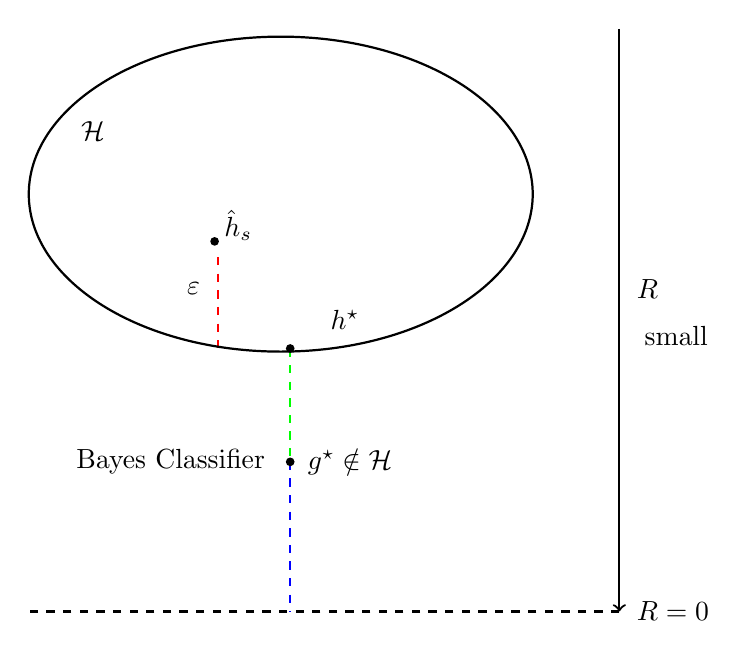
\begin{tikzpicture} [scale = 1] 
\draw[green, dashed, thick] (4.52, 2.04) -- (4.52, 0.6);
\draw[blue, dashed, thick] (4.52, 0.6) -- (4.52, -1.3);
\draw[black, fill = black, thick] (4.52, 0.6) circle [radius = 0.04];
\node[black, right] at (4.62, 0.6){$g^\star  \notin \mathcal{H}$};
\node[black, left] at (4.42, 0.6){$\text{\;Bayes Classifier\;}$};
\draw[black, dashed, thick] (8.7, -1.3) -- (1.2, -1.3);
\node[black, left] at (3.5, 2.8){$\varepsilon$};
\draw[red, dashed, thick] (3.6, 3.2) -- (3.6, 2.0);
\node[black, right] at (4.91, 2.4){$h^\star $};
\node[black, right] at (3.56, 3.6){$\hat{h}_{s}$};
\node[black, right] at (1.74, 4.8){$\mathcal{H}$};
\draw[black, fill = black, thick] (3.56, 3.4) circle [radius = 0.04];
\draw[black, fill = black, thick] (4.52, 2.04) circle [radius = 0.04];
\draw[black, thick] (4.4, 4.0) ellipse (3.2 and 2.0);
\node[black, right] at (8.8, -1.3){$R  = 0$};
\node[black, right] at (8.8, 2.2){$\text{\;small\;}$};
\node[black, right] at (8.8, 2.8){$R $};
\draw[black, ->, thick] (8.7, 6.1) -- (8.7, -1.3);
\end{tikzpicture} 
\end{figure}
(red) Estimation error: $R\left(\hat{h}_{s}\right)  - R\left(h^\star \right)$
\\* (green) Apprimation error: $R\left(h^\star \right)  - R\left(g^{\text{\;Bayes\;}}\right)$
\\* (blue) Bayes error: $R\left(g^{\text{\;Bayes\;}}\right) $
\newline \newline
\begin{align*}
P_{X} &= \text{\;Unif\;} \left[0, 1\right]^{2}
\\ &P_{X Y}
\end{align*}
\begin{figure}[H] \centering 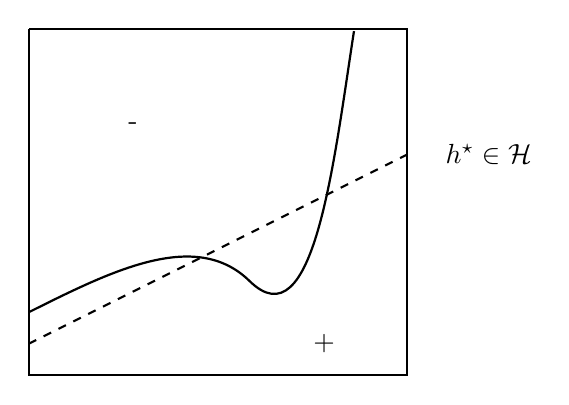
\begin{tikzpicture} [scale = 1] 
\node[black, right] at (5.09, 2.0){+};
\node[black, right] at (2.74, 4.8){-};
\node[black, right] at (6.77, 4.4){$h^\star  \in \mathcal{H}$};
\draw[black, dashed, thick] (1.6, 2.0) -- (6.4, 4.4);
\draw[black, thick] (1.6, 2.4).. controls(2.66, 2.93)and(3.72, 3.46)..(4.4, 2.8).. controls(5.22, 1.99)and(5.47, 4.29)..(5.73, 5.97);
\draw[black, thick] (1.6, 6.0) -- (1.6, 1.6) -- (6.4, 1.6) -- (6.4, 6.0) -- (1.6, 6.0);
\end{tikzpicture} 
\end{figure}
$\mathcal{H}$ linear
\begin{align*}
&P_{Y | X}
\\ 1 &> P\left(y = + | x \in + \text{\;region\;}\right) > \dfrac{1}{2}
\\ \dfrac{1}{2} &> P\left(y = + | x \in - \text{\;region\;}\right) > 0
\end{align*}
\begin{figure}[H] \centering 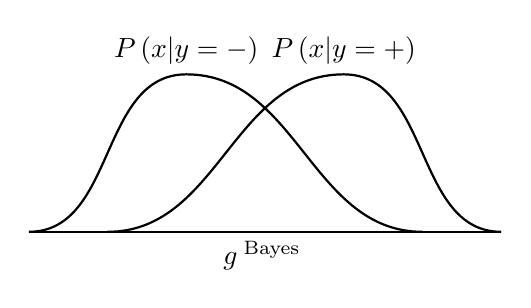
\begin{tikzpicture} [scale = 1] 
\draw[thick] (0.0, 0.0) -- (6.0, 0.0);
\node[below] at (3.0, 0.0){$g^{\text{\;Bayes\;}}$};
\draw[thick] (0.0, 0.0)to [out = 0, in = 180](2.0, 2.0)to [out = 0, in = 180](5.0, 0.0);
\draw[thick] (1.0, 0.0)to [out = 0, in = 180](4.0, 2.0)to [out = 0, in = 180](6.0, 0.0);
\node[above] at (2.0, 2.0){$P\left(x | y = -\right) $};
\node[above] at (4.0, 2.0){$P\left(x | y = +\right) $};
\end{tikzpicture} 
\end{figure}
\begin{align*}
\mathcal{H} &= \left\{\text{sign}\left[\sin\left(\alpha x\right)\right] : \alpha \in \left[1, 2\right]\right\}
\end{align*}
\begin{align*}
&g^{\text{\;Bayes\;}} \in \arg\displaystyle\max_{y \in Y} P\left(y | x\right) 
\end{align*}
Consider $\mathcal{H}_{1}, \mathcal{H}_{2}, ...$
\begin{align*}
VC\left(\mathcal{H}_{i}\right)  &< \infty, \;\forall\; i \in N 
\end{align*}
\begin{align*}
&  \mathbb{P}\left(\displaystyle\sup_{h \in \mathcal{H}} R\left(h\right) - \hat{R}_{s}\left(h\right) > \varepsilon\left(n, \delta\right)\right) \leq  \delta
\\ &\Rightarrow  \mathbb{P}\left(\displaystyle\sup_{h \in \mathcal{H}_{i}} R\left(h\right) - \hat{R}_{s}\left(h\right) > \varepsilon\left(n, w_{i} \delta\right)\right) \leq  w_{i} \delta, \;\forall\; i
\\ &  \mathbb{P}\left(\;\forall\; i, \displaystyle\sup_{h \in \mathcal{H}_{i}} R\left(h\right) - \hat{R}_{s}\left(h\right) > \varepsilon\left(n, w_{i} \delta\right)\right) \leq  \left(\displaystyle\sum_{i=1}^{\infty} w_{i}\right) \delta, \;\forall\; i
\end{align*}
where $\displaystyle\sum_{i=1}^{\infty} w_{i} \leq  1, w_{i} > 0$
\newline \newline
\begin{align*}
R\left(h\right)  - \hat{R}_{s}\left(h\right) &\leq  \varepsilon_{i}\left(n, w_{i} \delta\right)
\\ R\left(h\right)  &\leq  \hat{R}_{s}\left(h\right) + \varepsilon_{i}\left(n, w_{i} \delta\right)
\end{align*}
"Alg $1$"
\begin{align*}
&\hat{h}_{s} \in \arg\displaystyle\inf_{h \in \cup_{i=1}^{\infty} \mathcal{H}_{i}} \hat{R}_{s}\left(h\right) + \displaystyle\min_{i : h \in \mathcal{H}_{i}} \varepsilon_{i}\left(n, w_{i} \delta\right)
\end{align*}
\begin{figure}[H] \centering \begin{tikzpicture} [scale = 1] 
\draw[black, dashed, thick] (6.25, 1.6) -- (6.25, 0.6);
\draw[black, dashed, thick] (4.4, 4.0) -- (4.4, 2.0);
\node[black, right] at (8.19, 1.2){$x $};
\node[black, right] at (7.41, 8.0){$g  \geq  f$};
\node[black, right] at (8.05, 5.2){$f\left(x\right) $};
\draw[black, thick] (1.2, 6.8).. controls(1.76, 6.53)and(2.32, 6.26)..(2.94, 5.31).. controls(4.57, 2.81)and(6.6, 5.11)..(8.64, 7.32);
\draw[black, thick] (1.6, 4.4).. controls(3.02, 3.44)and(4.44, 2.48)..(5.68, 1.04).. controls(6.82, -0.3)and(7.81, 2.71)..(8.8, 4.8);
\draw[black, <->, thick] (2.0, 7.2) -- (2.0, 1.6) -- (8.8, 1.6);
\end{tikzpicture} 
\end{figure}
"Alg $2" \leftarrow$ Stuctural Risk Minimization
\begin{align*}
i^\star \left(h\right) &= \left[ \arg\displaystyle\min_{i = 1, 2, ...} h \in \mathcal{H}_{i} \right], \hat{h}_{s} \in \arg\displaystyle\inf_{h} \hat{R}_{s}\left(h\right) + \varepsilon_{i^\star \left(h\right)}\left(n, w_{i^\star \left(h\right)} \delta\right)
\end{align*}
\begin{align*}
&\displaystyle\min_{\theta} \displaystyle\sum_{i=1}^{n} \ell\left(\theta, x_{i} y_{i}\right) + \dfrac{\lambda}{2} \left\|\theta\right\|^{2}
\\ &\displaystyle\min_{\theta} \displaystyle\sum_{i=1}^{n} \ell\left(\theta, x_{i} y_{i}\right) + \dfrac{\lambda}{2} \left\|\theta - 86\right\|^{2}
\end{align*}



\section{Lecture $10$} 
Structural Risk Minimization
\\* Input: $\mathcal{H}_{1}, \mathcal{H}_{2}, ...$ each with finite VC
\begin{align*}
w_{1}, w_{2}, ..., \text{\;such that\;} \displaystyle\sum_{i=1}^{\infty} w_{i} &\leq  1, w_{i} \geq  0
\\ \varepsilon_{i}\left(N, w_{i} \delta\right) &\approx \sqrt{\dfrac{VC\left(\mathcal{H}_{i}\right)  + \log \dfrac{1}{w_{i} \delta}}{N}}
\\ \mathbb{P}_{s}\left(\displaystyle\sup_{h \in \mathcal{H}_{i}} R\left(h\right) - \hat{R}\left(h\right) > \varepsilon_{i}\left(N, w_{i} \delta\right)\right) &< w_{i} \delta
\end{align*}
Union bound over $i  = 1, 2, ...$
\begin{align*}
\mathbb{P}_{s}\left(\exists i, \displaystyle\sup_{h \in \mathcal{H}_{i}} R\left(h\right) - \hat{R}\left(h\right) > \varepsilon_{i}\left(N, w_{i} \delta\right)\right) &< \left(\displaystyle\sum_{i=1}^{\infty} w_{i}\right) \delta
\\ \mathbb{P}_{s}\left(\;\forall\; i, \displaystyle\sup_{h \in \mathcal{H}_{i}} R\left(h\right) - \hat{R}\left(h\right) \leq  \varepsilon_{i}\left(N, w_{i} \delta\right)\right) &\geq  1 - \left(\displaystyle\sum_{i=1}^{\infty} w_{i}\right) \delta \stackrel{\left(\displaystyle\sum_{i} w_{i} \delta \leq  1\right)}{\geq} 1 - \delta
\end{align*}
For each $\mathcal{H}_{i}$
\begin{align*}
\;\forall\; \varepsilon, \delta, P, \exists N, \;\forall\; n &> N 
\\ \mathbb{P}_{s \sim  P^{n}}\left(\displaystyle\sup_{h \in \mathcal{H}_{i}} R\left(h\right) - \hat{R}_{s}\left(h\right) > \varepsilon\right) &< \delta
\\ N  &\approx \dfrac{VC\left(\mathcal{H}_{i}\right)  + \log \dfrac{1}{\delta}}{\varepsilon^{2}}
\\ \varepsilon_{i}\left(w, \delta\right) &\approx \sqrt{\dfrac{VC\left(\mathcal{H}_{i}\right)  + \log \dfrac{1}{\delta}}{N}}
\end{align*}
SRM:
\begin{align*}
&\hat{h} ^{\text{\;SRM\;}} \in \arg\displaystyle\min_{i, h \in \mathcal{H}_{i}} \hat{R}\left(h\right) + \varepsilon_{i}\left(N, w_{i} \delta\right)
\end{align*}
Special Case of SRM
\\* Assumption: $\mathcal{H}$ countable
\begin{align*}
\mathcal{H} &= \left\{h_{1}, h_{2}, ...\right\}
\\ &= \left\{h_{1}\right\} \cup \left\{h_{2}\right\} \cup ...
\\ \mathcal{H}_{1} &= \left\{h_{1}\right\}, \mathcal{H}_{2} = \left\{h_{2}\right\} ...
\end{align*}
Need $w_{i}$ for $\mathcal{H}_{i}$, equiv denote as $w_{h}, h \in \mathcal{H}$
\begin{align*}
\displaystyle\sum_{h \in \mathcal{H}} w_{i} &\leq  1, w_{h} \geq  0 \;\forall\; h \in \mathcal{H}
\end{align*}
SRM
\begin{align*}
\hat{h} ^{\text{\;SRM\;}} \in \arg\displaystyle\min_{h \in \mathcal{H}} \hat{R}\left(h\right) + \varepsilon_{i}\left(N, w_{i} \delta\right) &= \arg\displaystyle\min_{h \in \mathcal{H}} \hat{R}\left(h\right) + \sqrt{\dfrac{\log \dfrac{1}{w_{i}} + \log \dfrac{2}{\delta}}{2 N}}
\end{align*}
$\mathcal{H}_{i}$ singleton $\Rightarrow $ Hoeffding's
\begin{align*}
\varepsilon_{i} &= \sqrt{\dfrac{\log \dfrac{2}{w_{i} \delta}}{2 N}}
\end{align*}
$\boxed{\text{\;Special\;} ^{2} \text{\;case\;}}$ prefix binary code
\newline \newline
\begin{figure}[H] \centering 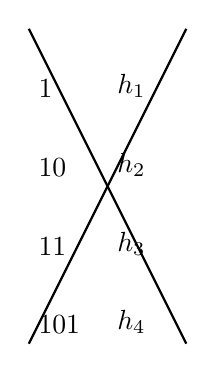
\begin{tikzpicture} [scale = 1] 
\node[above right] at (0.0, 0.0){$101$};
\node[above right] at (1.0, 0.0){$h_{4}$};
\node[above right] at (0.0, 1.0){$11$};
\node[above right] at (1.0, 1.0){$h_{3}$};
\node[above right] at (0.0, 2.0){$10$};
\node[above right] at (1.0, 2.0){$h_{2}$};
\node[above right] at (0.0, 3.0){$1$};
\node[above right] at (1.0, 3.0){$h_{1}$};
\draw[thick] (0.0, 0.0) -- (2.0, 4.0);
\draw[thick] (0.0, 4.0) -- (2.0, 0.0);
\end{tikzpicture} \end{figure}
\begin{figure}[H] \centering 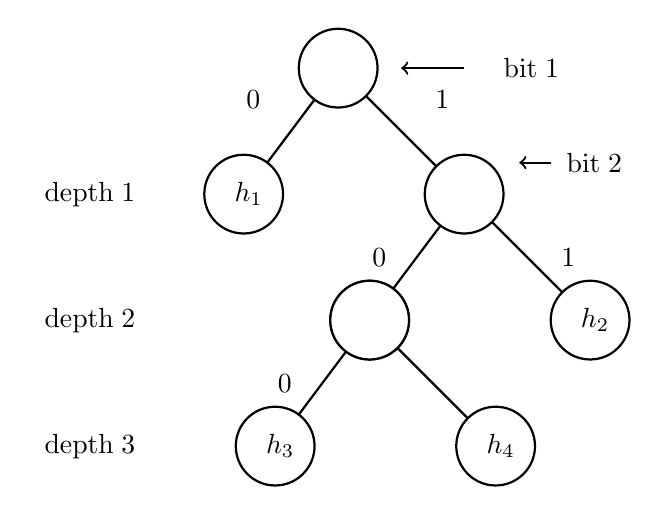
\begin{tikzpicture} [scale = 1] 
\draw[black, ->, thick] (7.5, 6.8) -- (7.1, 6.8);
\draw[black, ->, thick] (6.4, 8.0) -- (5.6, 8.0);
\node[black, right] at (7.48, 6.8){$\text{\;bit\;} 2$};
\node[black, right] at (6.68, 8.0){$\text{\;bit\;} 1$};
\node[black, right] at (0.85, 3.2){$\text{\;depth\;} 3$};
\node[black, right] at (0.85, 4.8){$\text{\;depth\;} 2$};
\node[black, right] at (0.85, 6.4){$\text{\;depth\;} 1$};
\node[black, right] at (3.91, 4.0){$0$};
\node[black, right] at (7.51, 5.6){$1$};
\node[black, right] at (5.11, 5.6){$0$};
\node[black, right] at (5.91, 7.6){$1$};
\node[black, right] at (3.51, 7.6){$0$};
\draw[black, thick] (5.2, 4.8) -- (6.8, 3.2);
\draw[black, thick] (5.2, 4.8) -- (4.0, 3.2);
\draw[black, thick] (6.4, 6.4) -- (8.0, 4.8);
\draw[black, thick] (6.4, 6.4) -- (5.2, 4.8);
\draw[black, thick] (4.8, 8.0) -- (6.4, 6.4);
\draw[black, thick] (4.8, 8.0) -- (3.6, 6.4);
\draw[black, fill = white, thick] (4.8, 8.0) circle [radius = 0.5];
\draw[black, fill = white, thick] (3.6, 6.4) circle [radius = 0.5];
\draw[black, fill = white, thick] (6.4, 6.4) circle [radius = 0.5];
\draw[black, fill = white, thick] (5.2, 4.8) circle [radius = 0.5];
\draw[black, fill = white, thick] (8.0, 4.8) circle [radius = 0.5];
\draw[black, fill = white, thick] (4.0, 3.2) circle [radius = 0.5];
\draw[black, fill = white, thick] (6.8, 3.2) circle [radius = 0.5];
\draw[black, fill = white, thick] (5.2, 4.8) circle [radius = 0.5];
\node[black, right] at (6.56, 3.2){$h_{4}$};
\node[black, right] at (3.76, 3.2){$h_{3}$};
\node[black, right] at (7.76, 4.8){$h_{2}$};
\node[black, right] at (3.36, 6.4){$h_{1}$};
\end{tikzpicture} 
\end{figure}
\begin{figure}[H] \centering 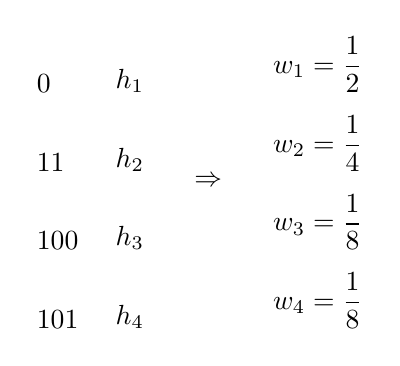
\begin{tikzpicture} [scale = 1] 
\node[above right] at (0.0, 0.0){$101$};
\node[above right] at (1.0, 0.0){$h_{4}$};
\node[above right] at (0.0, 1.0){$100$};
\node[above right] at (1.0, 1.0){$h_{3}$};
\node[above right] at (0.0, 2.0){$11$};
\node[above right] at (1.0, 2.0){$h_{2}$};
\node[above right] at (0.0, 3.0){$0$};
\node[above right] at (1.0, 3.0){$h_{1}$};
\node[right] at (2.0, 2.0){$\Rightarrow $};
\node[above right] at (3.0, 0.0){$w_{4} = \dfrac{1}{8}$};
\node[above right] at (3.0, 1.0){$w_{3} = \dfrac{1}{8}$};
\node[above right] at (3.0, 2.0){$w_{2} = \dfrac{1}{4}$};
\node[above right] at (3.0, 3.0){$w_{1} = \dfrac{1}{2}$};
\end{tikzpicture} \end{figure}
\begin{align*}
w_{h} :&= \dfrac{1}{2^{\text{\;depth\;} \left(h\right)}}
\end{align*}
Kreft's Thm
\begin{align*}
\displaystyle\sum_{h \in \mathcal{H}} w_{h} &\leq  1
\end{align*}
\begin{align*}
&\arg\displaystyle\min \hat{R}\left(h\right) + \sqrt{\dfrac{\text{\;depth\;} \left(h\right) \log 2 + \log \dfrac{1}{\delta}}{2 N}}
\end{align*}
minimum description length (MDL)
\\* $\Rightarrow $ Occam's Razor
\newline \newline
PAC-Bayes bound
\\* Set prior $P $ over $\mathcal{H}$
\\* For any $Q  = A\left(S \right)$ over $\mathcal{H}$ that learner produces (i.e. equiv of $\hat{h} ^{\text{\;ERM\;}}$)
\begin{align*}
R\left(Q\right)  :&= \mathbb{E}_{\left(x, y\right) \sim  P_{\text{\;dist\;}}} \mathbb{E}_{h \sim  Q} \ell\left(h\left(x\right), y\right)
\end{align*}



\section{Lecture $11$} 
PAC-Bayes bound
\\* Prior $P $ over $\mathcal{H}$, loss $\ell \in \left[0, 1\right]$
\\* Risk $R\left(h\right)  = \mathbb{E}_{P_{X Y}} \ell\left(h\left(x\right), y\right), \hat{R}_{s}\left(h\right) = \dfrac{1}{| S | = n} \displaystyle\sum_{i=1}^{n} \ell\left(h\left(x_{i}\right), y_{i}\right)$
\\* "Gibbs classifier" $h  \sim  P $
\begin{align*}
R\left(P\right)  &= \mathbb{E}_{h \sim  P} R\left(h\right) , \hat{R}_{s}\left(P\right) = \mathbb{E}_{h \sim  P} \hat{R}_{s}\left(h\right)
\end{align*}
Sample $S  \sim  P_{X Y}^{n}, A\left(S\right)  := Q $ distribution over $\mathcal{H}$
\newline \newline
\begin{thm} \label{thm:pacbb} 
$P $ given, $\;\forall\; P_{XY}, \ell \in \left[0, 1\right], \varepsilon, \delta$,
\begin{align*}
\mathbb{P}_{S \sim  P_{XY}^{n}}\left(\;\forall\; Q , R\left(Q\right) \leq  \hat{R}_{s}\left(Q\right) + \sqrt{\dfrac{KL  \left(Q \| P\right) + \log \dfrac{n}{\delta}}{2 \left(n - 1\right)}}\right) &\geq  1 - \delta
\\ KL\left(Q \| P\right)  :&= \displaystyle\sum_{h \in \mathcal{H}} Q\left(h\right) \log \dfrac{Q\left(h\right)}{P\left(h\right)}
\end{align*}
Let $Q_{1}$ concentrated on $\hat{h}_{s}^{\text{\;ERM\;}}, Q_{1}$ minimizes $\hat{R}_{s}\left(Q\right)$
\begin{align*}
KL\left(Q_{1} \| P\right)  &= Q\left(\hat{h}_{s}^{\text{\;ERM\;}}\right) \log \dfrac{Q\left(\hat{h}_{s}^{\text{\;ERM\;}}\right)}{P\left(\hat{h}_{s}^{\text{\;ERM\;}}\right)} = \log \dfrac{1}{P\left(\hat{h}_{s}^{\text{\;ERM\;}}\right)}
\\ \lim_{x \to  0} x \log x &= \lim_{x \to  0} \dfrac{\left(\log x\right)'}{\left(\dfrac{1}{x}\right)'} = \dfrac{\dfrac{1}{x}}{- \dfrac{1}{x^{2}}} = - x = 0
\end{align*}\end{thm}
(read textbook for proof)
\newline \newline

\subsection{Rademacher Complexity}
\begin{align*}
\mathcal{F} :&= \ell \circ \mathcal{H} = \left\{f\left(\cdot , \cdot \right) := \ell\left(h\left(\cdot \right), \cdot \right), h \in \mathcal{H}\right\}
\\ R\left(f\right)  &= \mathbb{E}_{\left(x, y\right) \sim  P_{XY}} f\left(x, y\right), \hat{R}_{s}\left(f\right) = \dfrac{1}{n} \displaystyle\sum_{\left(x, y\right) \in S} f\left(x, y\right) 
\end{align*}
\begin{df} \label{df:rad} 
Rademacher Complexity of $\mathcal{F}$
\begin{align*}
\mathbb{R}\left(\mathcal{F} \circ S\right) :&= \dfrac{1}{n} \mathbb{E}_{\vec{\sigma}} \displaystyle\sup_{f \in \mathcal{H}} \vec{\sigma}^{T} \vec{f}_{s}
\end{align*}
Depends on $S $, (alos $n $ )
\newline \newline\end{df}
\begin{align*}
\left[\sigma_{1}, ..., \sigma_{n}\right] :&= \vec{\sigma} , \sigma_{i} \in\left\{-1, 1\right\}, P\left(\sigma_{i} = 1\right)  = \dfrac{1}{2} \;\forall\; i 
\\ &\begin{bmatrix} f\left(x_{1}, y_{1}\right) \\ ... \\ f\left(x_{n}, y_{n}\right) \end{bmatrix} \left(x_{i}, y_{i}\right) \in S, f \in \mathcal{F}
\end{align*}
\begin{thm} \label{thm:radc} 
$26.5 \left(3\right)$ loss bound, $| \ell\left(\cdot \right) | \leq  c $
\begin{align*}
\;\forall\; h^\star  \in \mathcal{H}, \text{\;wp\;} &\geq  1 - \delta, R\left(\hat{h}_{s}^{\text{\;ERM\;}}\right) \leq  R\left(h^\star \right) + 2 \mathbb{R}\left(\mathcal{F} \circ S\right) + 5 c \sqrt{\dfrac{2 \log \dfrac{8}{\delta}}{n}}
\end{align*}
data dependent bound
\newline \newline\end{thm}




\section{Lecture $12$} 
\begin{figure}[H] \centering 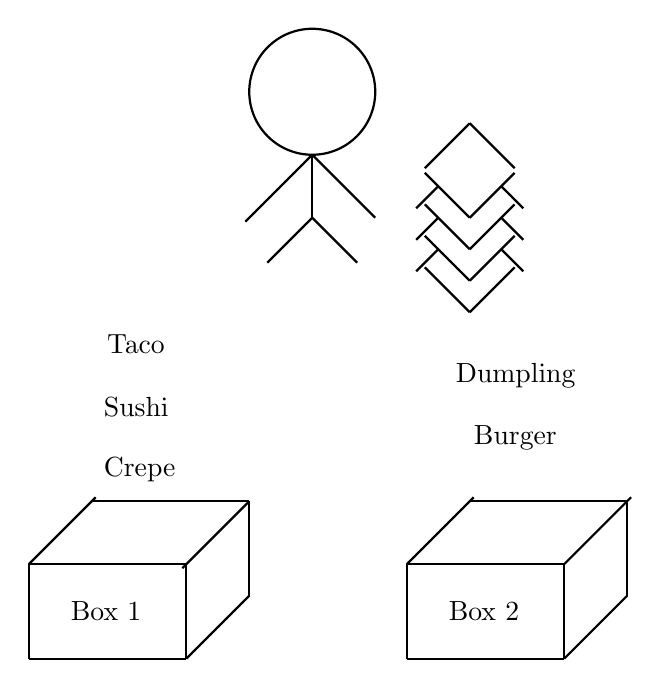
\begin{tikzpicture} [scale = 1] 
\node[black, right] at (2.03, 4.0){Crepe};
\node[black, right] at (6.73, 4.4){Burger};
\node[black, right] at (6.5, 5.2){Dumpling};
\node[black, right] at (2.03, 4.8){Sushi};
\node[black, right] at (2.07, 5.6){Taco};
\node[black, right] at (6.41, 2.2){Box $2$};
\node[black, right] at (1.61, 2.2){Box $1$};
\draw[black, thick] (8.0, 1.6) -- (8.8, 2.4);
\draw[black, thick] (8.8, 3.6) -- (8.8, 2.4);
\draw[black, thick] (8.0, 2.8) -- (8.85, 3.65);
\draw[black, thick] (6.8, 3.6) -- (8.8, 3.6);
\draw[black, thick] (6.0, 2.8) -- (6.85, 3.65);
\draw[black, thick] (6.0, 1.6) -- (8.0, 1.6);
\draw[black, thick] (8.0, 2.8) -- (8.0, 1.6);
\draw[black, thick] (6.0, 2.8) -- (8.0, 2.8);
\draw[black, thick] (6.0, 2.8) -- (6.0, 1.6);
\draw[black, thick] (3.2, 1.6) -- (3.6, 2.0) -- (4.0, 2.4);
\draw[black, thick] (4.0, 3.6) -- (4.0, 2.8) -- (4.0, 2.4);
\draw[black, thick] (4.0, 3.6) -- (3.15, 2.75);
\draw[black, thick] (2.0, 3.6) -- (4.0, 3.6);
\draw[black, thick] (1.2, 2.8) -- (2.05, 3.65);
\draw[black, thick] (1.2, 1.6) -- (3.2, 1.6);
\draw[black, thick] (3.2, 2.8) -- (3.2, 1.6);
\draw[black, thick] (1.2, 2.8) -- (3.2, 2.8);
\draw[black, thick] (1.2, 2.8) -- (1.2, 1.6);
\draw[black, thick] (7.2, 6.8) -- (7.48, 6.52);
\draw[black, thick] (6.8, 6.0) -- (7.37, 6.57);
\draw[black, thick] (6.8, 6.0) -- (6.23, 6.57);
\draw[black, thick] (6.4, 6.8) -- (6.12, 6.52);
\draw[black, thick] (7.2, 7.2) -- (7.48, 6.92);
\draw[black, thick] (6.8, 6.4) -- (7.37, 6.97);
\draw[black, thick] (6.8, 6.4) -- (6.23, 6.97);
\draw[black, thick] (6.4, 7.2) -- (6.12, 6.92);
\draw[black, thick] (7.2, 7.6) -- (7.48, 7.32);
\draw[black, thick] (6.8, 6.8) -- (7.37, 7.37);
\draw[black, thick] (6.8, 6.8) -- (6.23, 7.37);
\draw[black, thick] (6.4, 7.6) -- (6.12, 7.32);
\draw[black, thick] (6.8, 7.2) -- (7.37, 7.77);
\draw[black, thick] (6.8, 7.2) -- (6.23, 7.77);
\draw[black, thick] (6.8, 8.4) -- (7.37, 7.83);
\draw[black, thick] (6.8, 8.4) -- (6.23, 7.83);
\draw[black, thick] (4.8, 7.2) -- (5.37, 6.63);
\draw[black, thick] (4.8, 7.2) -- (4.23, 6.63);
\draw[black, thick] (4.8, 8.0) -- (5.6, 7.2);
\draw[black, thick] (4.8, 8.0) -- (3.95, 7.15);
\draw[black, thick] (4.8, 8.0) -- (4.8, 7.2);
\draw[black, thick] (4.8, 8.8) ellipse (0.8 and 0.8);
\end{tikzpicture} 
\end{figure}
$X  =$ vocabulary
\begin{align*}
&h  \in \underbrace{\mathcal{H}}_{\text{\;all rules in your mind\;}}, X \to  \left\{\text{\;Box1\;} , \text{\;Box2\;}\right\}
\\ \dfrac{1}{m} &= \displaystyle\sum_{j=1}^{m} \displaystyle\sup_{h \in \mathcal{H}} \displaystyle\sum_{i=1}^{5}  \sigma_{i}^{\left(j\right)} h\left(x_{i}\right)
\\ &\approx \mathbb{E}_{\sigma_{1} ... \sigma_{5}} \displaystyle\sup_{h \in \mathcal{H}} \vec{\sigma}^{T} \vec{h}
\end{align*}
\begin{figure}[H] \centering 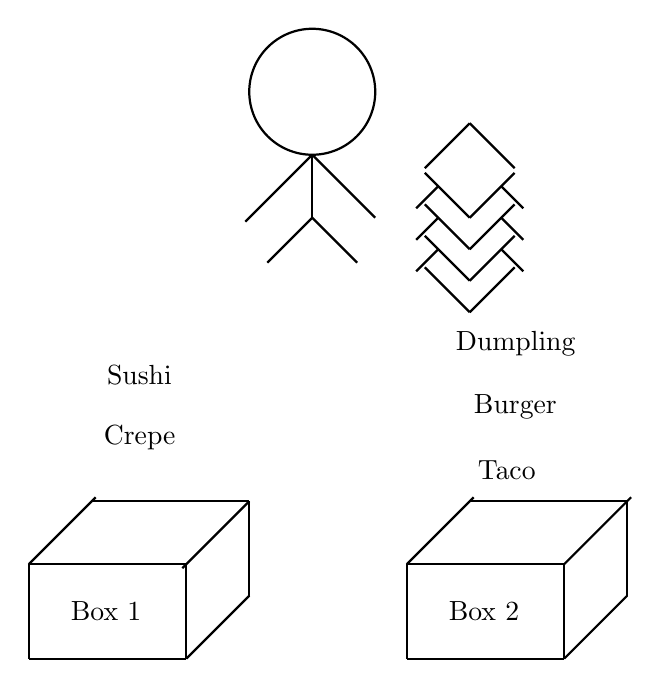
\begin{tikzpicture} [scale = 1] 
\node[black, right] at (6.78, 4.0){Taco};
\node[black, right] at (6.73, 4.8){Burger};
\node[black, right] at (6.5, 5.6){Dumpling};
\node[black, right] at (2.03, 4.4){Crepe};
\node[black, right] at (2.07, 5.2){Sushi};
\node[black, right] at (6.41, 2.2){Box $2$};
\node[black, right] at (1.61, 2.2){Box $1$};
\draw[black, thick] (8.0, 1.6) -- (8.8, 2.4);
\draw[black, thick] (8.8, 3.6) -- (8.8, 2.4);
\draw[black, thick] (8.0, 2.8) -- (8.85, 3.65);
\draw[black, thick] (6.8, 3.6) -- (8.8, 3.6);
\draw[black, thick] (6.0, 2.8) -- (6.85, 3.65);
\draw[black, thick] (6.0, 1.6) -- (8.0, 1.6);
\draw[black, thick] (8.0, 2.8) -- (8.0, 1.6);
\draw[black, thick] (6.0, 2.8) -- (8.0, 2.8);
\draw[black, thick] (6.0, 2.8) -- (6.0, 1.6);
\draw[black, thick] (3.2, 1.6) -- (3.6, 2.0) -- (4.0, 2.4);
\draw[black, thick] (4.0, 3.6) -- (4.0, 2.8) -- (4.0, 2.4);
\draw[black, thick] (4.0, 3.6) -- (3.15, 2.75);
\draw[black, thick] (2.0, 3.6) -- (4.0, 3.6);
\draw[black, thick] (1.2, 2.8) -- (2.05, 3.65);
\draw[black, thick] (1.2, 1.6) -- (3.2, 1.6);
\draw[black, thick] (3.2, 2.8) -- (3.2, 1.6);
\draw[black, thick] (1.2, 2.8) -- (3.2, 2.8);
\draw[black, thick] (1.2, 2.8) -- (1.2, 1.6);
\draw[black, thick] (7.2, 6.8) -- (7.48, 6.52);
\draw[black, thick] (6.8, 6.0) -- (7.37, 6.57);
\draw[black, thick] (6.8, 6.0) -- (6.23, 6.57);
\draw[black, thick] (6.4, 6.8) -- (6.12, 6.52);
\draw[black, thick] (7.2, 7.2) -- (7.48, 6.92);
\draw[black, thick] (6.8, 6.4) -- (7.37, 6.97);
\draw[black, thick] (6.8, 6.4) -- (6.23, 6.97);
\draw[black, thick] (6.4, 7.2) -- (6.12, 6.92);
\draw[black, thick] (7.2, 7.6) -- (7.48, 7.32);
\draw[black, thick] (6.8, 6.8) -- (7.37, 7.37);
\draw[black, thick] (6.8, 6.8) -- (6.23, 7.37);
\draw[black, thick] (6.4, 7.6) -- (6.12, 7.32);
\draw[black, thick] (6.8, 7.2) -- (7.37, 7.77);
\draw[black, thick] (6.8, 7.2) -- (6.23, 7.77);
\draw[black, thick] (6.8, 8.4) -- (7.37, 7.83);
\draw[black, thick] (6.8, 8.4) -- (6.23, 7.83);
\draw[black, thick] (4.8, 7.2) -- (5.37, 6.63);
\draw[black, thick] (4.8, 7.2) -- (4.23, 6.63);
\draw[black, thick] (4.8, 8.0) -- (5.6, 7.2);
\draw[black, thick] (4.8, 8.0) -- (3.95, 7.15);
\draw[black, thick] (4.8, 8.0) -- (4.8, 7.2);
\draw[black, thick] (4.8, 8.8) ellipse (0.8 and 0.8);
\end{tikzpicture} 
\end{figure}
\begin{figure}[H] \centering 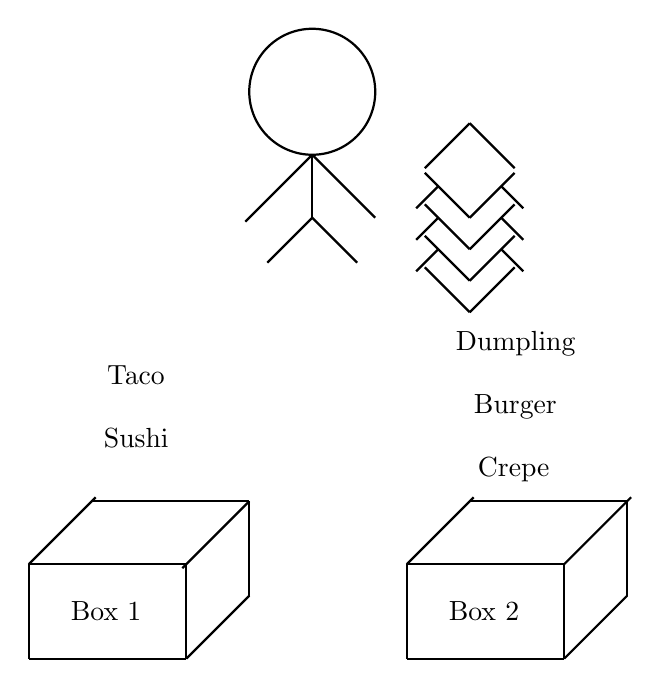
\begin{tikzpicture} [scale = 1] 
\node[black, right] at (6.78, 4.0){Crepe};
\node[black, right] at (6.73, 4.8){Burger};
\node[black, right] at (6.5, 5.6){Dumpling};
\node[black, right] at (2.03, 4.4){Sushi};
\node[black, right] at (2.07, 5.2){Taco};
\node[black, right] at (6.41, 2.2){Box $2$};
\node[black, right] at (1.61, 2.2){Box $1$};
\draw[black, thick] (8.0, 1.6) -- (8.8, 2.4);
\draw[black, thick] (8.8, 3.6) -- (8.8, 2.4);
\draw[black, thick] (8.0, 2.8) -- (8.85, 3.65);
\draw[black, thick] (6.8, 3.6) -- (8.8, 3.6);
\draw[black, thick] (6.0, 2.8) -- (6.85, 3.65);
\draw[black, thick] (6.0, 1.6) -- (8.0, 1.6);
\draw[black, thick] (8.0, 2.8) -- (8.0, 1.6);
\draw[black, thick] (6.0, 2.8) -- (8.0, 2.8);
\draw[black, thick] (6.0, 2.8) -- (6.0, 1.6);
\draw[black, thick] (3.2, 1.6) -- (3.6, 2.0) -- (4.0, 2.4);
\draw[black, thick] (4.0, 3.6) -- (4.0, 2.8) -- (4.0, 2.4);
\draw[black, thick] (4.0, 3.6) -- (3.15, 2.75);
\draw[black, thick] (2.0, 3.6) -- (4.0, 3.6);
\draw[black, thick] (1.2, 2.8) -- (2.05, 3.65);
\draw[black, thick] (1.2, 1.6) -- (3.2, 1.6);
\draw[black, thick] (3.2, 2.8) -- (3.2, 1.6);
\draw[black, thick] (1.2, 2.8) -- (3.2, 2.8);
\draw[black, thick] (1.2, 2.8) -- (1.2, 1.6);
\draw[black, thick] (7.2, 6.8) -- (7.48, 6.52);
\draw[black, thick] (6.8, 6.0) -- (7.37, 6.57);
\draw[black, thick] (6.8, 6.0) -- (6.23, 6.57);
\draw[black, thick] (6.4, 6.8) -- (6.12, 6.52);
\draw[black, thick] (7.2, 7.2) -- (7.48, 6.92);
\draw[black, thick] (6.8, 6.4) -- (7.37, 6.97);
\draw[black, thick] (6.8, 6.4) -- (6.23, 6.97);
\draw[black, thick] (6.4, 7.2) -- (6.12, 6.92);
\draw[black, thick] (7.2, 7.6) -- (7.48, 7.32);
\draw[black, thick] (6.8, 6.8) -- (7.37, 7.37);
\draw[black, thick] (6.8, 6.8) -- (6.23, 7.37);
\draw[black, thick] (6.4, 7.6) -- (6.12, 7.32);
\draw[black, thick] (6.8, 7.2) -- (7.37, 7.77);
\draw[black, thick] (6.8, 7.2) -- (6.23, 7.77);
\draw[black, thick] (6.8, 8.4) -- (7.37, 7.83);
\draw[black, thick] (6.8, 8.4) -- (6.23, 7.83);
\draw[black, thick] (4.8, 7.2) -- (5.37, 6.63);
\draw[black, thick] (4.8, 7.2) -- (4.23, 6.63);
\draw[black, thick] (4.8, 8.0) -- (5.6, 7.2);
\draw[black, thick] (4.8, 8.0) -- (3.95, 7.15);
\draw[black, thick] (4.8, 8.0) -- (4.8, 7.2);
\draw[black, thick] (4.8, 8.8) ellipse (0.8 and 0.8);
\end{tikzpicture} 
\end{figure}
\begin{align*}
&\mathbb{R}\left(\mathcal{H}\right)
\end{align*}
\begin{figure}[H] \centering \begin{tikzpicture} [scale = 1] 
\draw[->, thick] (0.0, 0.0) -- (6.0, 0.0);
\draw[->, thick] (0.0, 0.0) -- (0.0, 3.0);
\node[right] at (6.2, 0.0){$n $};
\node[above] at (0.0, 3.2){$\mathbb{R}$};
\draw[thick] (0.2, 2.8)to [out = -45, in = 180](5.8, 0.2);
\end{tikzpicture} \end{figure}
\begin{align*}
&A  \subset \mathbb{R}^{n}
\\ \mathbb{R}\left(A\right) &= \dfrac{1}{n} \mathbb{E}_{\sigma_{1} ... \sigma_{n}} \displaystyle\sup_{a \in A} \vec{\sigma}^{T} a 
\end{align*}
Lemma $26.2, F  = \ell \circ \mathcal{H}$
\begin{align*}
\mathbb{E}_{s} \left[\displaystyle\sup_{f \in \mathcal{F}} R\left(f\right) - \hat{R}_{s}\left(f\right)\right] &\leq  2 \mathbb{E}_{s} \mathbb{R}\left(F \circ S\right)'
\end{align*}
Proof:
\begin{align*}
\displaystyle\sup_{f \in F} R\left(f\right) - \hat{R}_{s}\left(f\right) &\stackrel{\text{\;ghost\;} s'}{=} \displaystyle\sup_{f \in F} \mathbb{E}_{s'}\left[\hat{R}_{s'}\left(f\right) - \hat{R}_{s}\left(f\right)\right]
\\ &\stackrel{\text{\;Jensen's\;}}{\leq} \mathbb{E}_{s'} \displaystyle\sup_{f \in F} \left[\hat{R}_{s'}\left(f\right) - \hat{R}_{s}\left(f\right)\right]
\end{align*}
\begin{equation} \label{equation:radm} 
\mathbb{E}_{s} \left[\displaystyle\sup R f - \hat{R}_{s} f\right] \leq  \mathbb{E}_{s, s'} \displaystyle\sup_{f} \left[\hat{R}_{s'} f - \hat{R}_{s} f\right]
\end{equation}
\begin{align*}
S  &= \left\{z_{1}, ..., z_{n}\right\}
\\ S' &= \left\{z'_{1}, ..., z'_{n}\right\}
\\ \left(1\right) \text{\;RHS\;} &= \dfrac{1}{n} \mathbb{E}_{s', s} \displaystyle\sup_{f} \displaystyle\sum_{i=1}^{n} \left(f\left(z'_{i}\right) - f\left(z_{i}\right)\right) \stackrel{\text{\;introduce\;} \sigma = \left\{\sigma_{1}, ..., \sigma_{n}\right\}}{=} \dfrac{1}{n} \mathbb{E}_{s', s, \sigma} \displaystyle\sup_{f} \displaystyle\sum_{i=1}^{n} \sigma_{i} \left(f\left(z'_{i}\right) - f\left(z_{i}\right)\right)
\\ &\leq  \dfrac{1}{n} \mathbb{E}_{s', s, \sigma}\left\{\left[\displaystyle\sup_{f \in F} \displaystyle\sum_{i}^{n} \sigma_{i} f\left(z'_{i}\right)\right] + \left[\displaystyle\sup_{g \in F} \displaystyle\sum_{i}^{n} \sigma_{i} \left(-g\left(z_{i}\right)\right)\right]\right\}
\\ &= \mathbb{E}_{s} \mathbb{R}\left(F \circ S\right) + \mathbb{E}_{s} \mathbb{R}\left(F \circ S\right) = 2 \mathbb{E}_{s} \mathbb{R}\left(F \circ S\right)
\\ &  \mathbb{E}_{s', s} \displaystyle\sup_{f} f\left(z'_{1}\right) - f\left(z_{1}\right) + \displaystyle\sum_{i=2}^{n} \left(f\left(z'_{i}\right) - f\left(z_{i}\right)\right)
\\ &\stackrel{s, s' \text{\;iid\;}}{=} \mathbb{E}_{s', s} \displaystyle\sup_{f} f\left(z_{1}\right) - f\left(z'_{1}\right) + \displaystyle\sum_{i=2}^{n} \left(f\left(z'_{i}\right) - f\left(z_{i}\right)\right)
\\ &= \mathbb{E}_{s', s, \sigma_{1}} \displaystyle\sup_{f} \sigma_{1}\left(f\left(z'_{1}\right) - f\left(z_{1}\right)\right) + \displaystyle\sum_{i=2}^{n} \left(f\left(z'_{i}\right) - f\left(z_{i}\right)\right)
\end{align*}
\begin{align*}
\mathbb{P}_{s}\left(\overbrace{\displaystyle\sup_{f \in F} R\left(f\right) - \hat{R}_{s}\left(f\right)}^{X } \geq  \varepsilon\right) &\leq  \dfrac{\mathbb{E}\left[\displaystyle\sup\right]}{\varepsilon} \leq  \dfrac{2 \mathbb{E}_{s} \mathbb{R}\left(F \circ S\right)}{\varepsilon} := \delta
\\ &\Rightarrow  \varepsilon = \dfrac{2 \mathbb{E}_{s} \mathbb{R}\left(F \circ S\right)}{\delta}
\end{align*}
Markov ineq r.v. $\boxed{X  \geq  0} \;\forall\; a > 0$
\begin{align*}
P\left(X > a\right)  &\leq  \dfrac{\mathbb{E}\left[X\right]}{a}
\end{align*}
\begin{align*}
&\boxed{\text{\;VC style\;} \varepsilon, \varepsilon = \sqrt{\dfrac{VC  \left(\mathcal{H}\right) + \log \dfrac{1}{\delta}}{n}}}
\end{align*}
McDiarmid's Ineq, $f : V^{n} \to  \mathbb{R}, V \subseteq \mathbb{R}$
\\* foral $i \in \left[n\right], \;\forall\; x_{i}, x'_{i} \in V, \left|  f\left(x_{1}, x_{2}, ..., x_{i}, ..., x_{n}\right)  - f\left(x_{1}, x_{2}, ..., x'_{i}, ..., x_{n}\right)  \right| \leq  c $
\\* Lecture $X_{1}, ..., X_{n}$ be r.v. in $V $
\begin{align*}
\mathbb{P}\left(\left|  f\left(X_{1}, ..., X_{n}\right) - \mathbb{E} f\left(X_{1}, ..., X_{n}\right)  \right| \leq  c \sqrt{\left(\log \dfrac{2}{\delta}\right) \dfrac{n}{2}}\right) &\geq  1 - \delta
\end{align*}



\section{Lecture $13$} 
\begin{align*}
&\mathbb{P}_{s}\left(\displaystyle\sup_{f \in F} R\left(f\right) - \hat{R}_{s}\left(f\right) > \varepsilon\right)
\end{align*}
Lemma $26.2$
\begin{align*}
\mathbb{E}_{s} \left[\displaystyle\sup_{f \in F} R\left(f\right) - \hat{R}_{s}\left(f\right)\right] &\leq  2 \mathbb{E}_{s} \mathbb{R}\left(F \circ S\right)
\end{align*}
Assumption: $\left|  \ell  \right| \leq  c $
\\* McDiarmid's Ineq: For $f $ which satisfies $\left|  f\left(x_{1} ... x_{i} ... x_{n}\right) - f\left(x_{1} ... x'_{i} ... x_{n}\right)  \right| \leq  c , \;\forall\; x, i, x'_{i}$
\begin{align*}
\text{\;wp\;} &\geq  1 - \delta, \left|  f\left(X_{1} ... X_{n}\right) - \mathbb{E} f\left(X_{1} ... X_{n}\right)  \right| \leq  C_{0} \sqrt{\dfrac{n \log \dfrac{2}{\delta}}{2}}
\end{align*}
\begin{align*}
&  \displaystyle\sup_{f \in F} R\left(f\right) - \hat{R}_{s}\left(f\right) = \displaystyle\sup_{h \in \mathcal{H}} \mathbb{E}_{\left(x, y\right) \sim  P_{X Y}} \ell\left(h\left(x\right), y\right) - \dfrac{1}{n} \displaystyle\sum_{i=1}^{n} \ell\left(h\left(x_{i}\right), y_{i}\right)
\\ &  s  = \left(x_{1}, y_{1}\right), ..., \left(x_{n}, y_{n}\right)
\\ &\Rightarrow  C_{0} = \dfrac{2 C}{n}
\\ &\stackrel{\text{\;McDiarmid\;}}{\Rightarrow} \text{\;wp\;} \geq  1 - \delta, \left|  \left[\displaystyle\sup_{f \in F} R\left(f\right) - \hat{R}_{s}\left(f\right)\right] - \mathbb{E}_{s'}\left[\displaystyle\sup_{f \in F} R\left(f\right) - \hat{R}_{s'}\left(f\right)\right]  \right| \leq  \dfrac{2 c}{n} \sqrt{\dfrac{n \log \dfrac{2}{\delta}}{2}} = c \sqrt{\dfrac{2 \log \dfrac{2}{\delta}}{n}}
\\ &  \;\forall\; x, i, x'_{i} \to  \text{\;wp\;} \geq  1 - \delta, \displaystyle\sup_{f \in F} R\left(f\right) - \hat{R}_{s}\left(f\right) \leq  \mathbb{E}_{s'}\left[\displaystyle\sup_{f \in F} R\left(f\right) - \hat{R}_{s'}\left(f\right)\right] + c \sqrt{\dfrac{2 \log \dfrac{2}{\delta}}{n}}
\\ &\stackrel{\text{\;Lemma\;} 26.2}{\leq} 2 \mathbb{E}_{s'} \mathbb{R}\left(F \circ S'\right) + c \sqrt{\dfrac{2 \log \dfrac{2}{\delta}}{n}}
\end{align*}
Thm $26.5 \left(1\right)$
\newline \newline
\begin{align*}
&\boxed{\text{\;ERM\;} \arg\displaystyle\min_{h \in \mathcal{H}} \hat{R}_{s}\left(h\right)}
\end{align*}
\begin{align*}
\mathcal{H} &= \left\{h_{w,b} : X \to  Y , w \in \mathbb{R}^{d}, b \in \mathbb{R}, h_{w,b}\left(x\right) = \text{sign}\left(w^{T} x + b\right)\right\}
\\ &  X  \subseteq \mathbb{R}^{d}, Y = \left\{-1, 1\right\}
\end{align*}
\[ \text{sign}\left(z\right) =\left\{ \begin{array}{ll}
1,& \text{\;if\;} z\geq  0 \\
-1,& \text{\;if\;} z < 0 \\
\end{array}\right. \]
\begin{align*}
&  \left\{x  : w^{T} x + b = 0\right\}
\\ &  VC\left(\mathcal{H}\right)  = d  + 1
\end{align*}
\begin{figure}[H] \centering 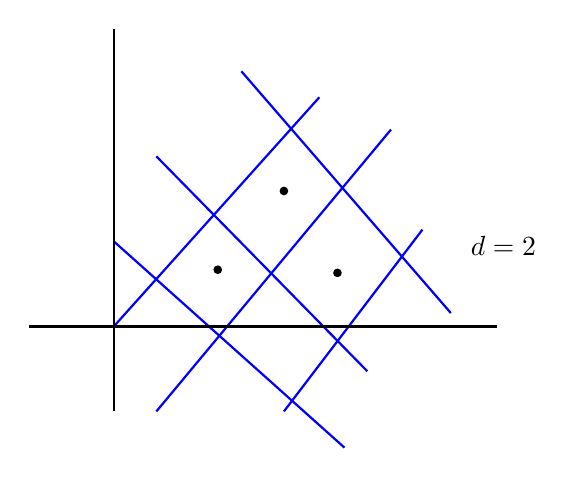
\begin{tikzpicture} [scale = 1] 
\draw[blue, thick] (3.24, 3.52) -- (6.17, 0.9);
\draw[blue, thick] (4.86, 5.68) -- (7.52, 2.61);
\draw[blue, thick] (3.78, 4.6) -- (6.46, 1.87);
\draw[blue, thick] (5.4, 1.36) -- (7.16, 3.67);
\draw[blue, thick] (3.78, 1.36) -- (6.76, 4.94);
\draw[blue, thick] (3.24, 2.44) -- (5.85, 5.35);
\node[black, right] at (7.65, 3.46){$d  = 2$};
\draw[black, fill = black, thick] (6.08, 3.12) circle [radius = 0.04];
\draw[black, fill = black, thick] (5.4, 4.16) circle [radius = 0.04];
\draw[black, fill = black, thick] (4.56, 3.16) circle [radius = 0.04];
\draw[black, thick] (3.24, 6.22) -- (3.24, 1.36);
\draw[black, thick] (2.16, 2.44) -- (8.1, 2.44);
\end{tikzpicture} 
\end{figure}
$\ell = 0-1$ loss
\\* Assume: $\exists h^\star  \in \mathcal{H}, \;\forall\; \left(x, y\right) \in S, y = h^\star \left(x\right)$
\newline \newline
(Batch) Perceptron Alg
\\* Init, $t  = 0, w_{0} = \vec{0} \in \mathbb{R}^{d}$
\\* pick $\left(x , y\right) \in S$
\\* if $\text{sign}\left(w_{t}^{T} x\right) \neq  y $
\begin{align*}
w_{t} &= w_{t} + y x 
\end{align*}
Terminates?$!$
\\* How many mistakes were made? $\neq  \hat{R}_{s}\left(h\right)$
\newline \newline
\begin{align*}
C  :&= \displaystyle\min_{i \in | S |} y_{i} \left(w^\star \right)^{T} x_{i}
\\ C  &> 0
\\ w^{\star\star} :&= \dfrac{w^\star }{c}
\\ \;\forall\; i, y_{i} \left(w^{\star\star}\right)^{T} x_{i} &\geq  1, \boxed{1}
\\ &  \boxed{B:= \displaystyle\min \| w \|, w \in \left\{w : \;\forall\; i \in S: y_{i} w^{T} x_{i} \geq  1\right\}}
\\ &  \boxed{w^\star  \in \arg\displaystyle\min}
\end{align*}
\begin{align*}
\dfrac{w_{t}^{T} w^\star }{\left\|w_{t}\right\| \left\|w^\star \right\|} &\stackrel{\cos}{\leq} 1
\\ w_{t+1}^{T} w^\star  - w_{t}^{T} w^\star  &= \left(w_{t+1} - w_{t}\right)^{T} w\cdot  = \left(y_{t} x_{t}\right)^{T} w^\star  \stackrel{\boxed{1}}{\geq} 1
\\ \displaystyle\sum_{t=0}^{T} \left(w_{t+1}^{T} w^\star  - w_{t}^{T} w^\star \right) &= w_{T+1}^{T} w^\star  - \underbrace{w_{0}^{T} w^\star }_{0} \geq  T , \boxed{2}
\end{align*}



\section{Lecture $14$} 
Batch Perceptron (Ch. $9$)
\\* Give $\left(x_{i}, y_{i}\right)_{i = 1:n}, Y  = \left\{-1, 1\right\}$
\\* Assume realizability $\exists w \in \mathbb{R}^{d} \;\forall\; i \in \left[n\right], y_{i} w^{T} x_{i} > 0$
\begin{align*}
&\Rightarrow  \exists w \;\forall\; -i, y_{i} w^{T} x_{i} \geq  1
\\ \bar{W} :&= \left\{w: \;\forall\; i, y_{i} w^{T} x_{i} \geq  1\right\}
\\ &w^\star  \in \arg\displaystyle\min_{w \in \bar{W}} \left\|w\right\|
\\ B  :&= \left\|w^\star \right\|
\end{align*}
Alg: $w_{0} = \emptyset$
\\* if $y_{i} w_{t}^{T} x_{t} \leq  0$ (misclassification)
\\* $w_{t+1} = w_{t} + y_{t} x_{t}$ (repeat)
\newline \newline
Claim: Alg makes bounded number of mistakes on any sequence $x_{t}, y_{t}$ (in training set)
\\* Proof:
\begin{align*}
\cos\left(w_{t+1}, w^\star \right) &= \dfrac{w_{t+1}^{T} w^\star }{\left\|w_{t+1}\right\| \cdot  \left\|w^\star \right\|} \leq  1
\end{align*}
step $1: w_{t+1}^{T} w^\star $ grows $O\left(t\right) $
\begin{align*}
w_{t+1}^{T} w^\star  &= \left(w_{t} + y_{t} x_{t}\right)^{T} w^\star  = w_{t}^{T} w^\star  + y_{t} \underbrace{x_{t}^{T} w^\star }_{\geq  1 \left(def  w^\star  \in \bar{W}\right)}
\\ &\Rightarrow  w_{t+1}^{T} w^\star  - w_{t}^{T} w^\star  \geq  1
\\ &\Rightarrow  \displaystyle\sum_{t=1}^{T-1} \left(w_{t+1}^{T} w^\star  - w_{t}^{T} w^\star \right) \geq  T 
\\ &\Rightarrow  w_{T}^{T} w^\star  - w_{0}^{T} w^\star  \geq  T 
\\ &\underbrace{\Rightarrow }_{w_{0} = \emptyset} w_{T}^{T} w^\star  \geq  T 
\end{align*}
step $2: \left\|w_{t+1}\right\| \sim  o\left(t\right) $
\begin{align*}
\left\|w_{t+1}\right\|^{2} &= \left\|w_{t} + y_{t} x_{t}\right\|^{2} = \left(w_{t} + y_{t} x_{t}\right)^{T} \left(w_{t} + y_{t} x_{t}\right)
\\ &= w_{t}^{T} w_{t} + 2 y_{t} w_{t}^{T} x_{t} + y_{t}^{2} x_{t}^{T} x_{t}
\\ &\underbrace{=}_{Y \in \left\{-1, 1\right\}} \left\|w_{t}\right\|^{2} + 2 \underbrace{y_{t} w_{t}^{T} x_{t}}_{\text{\;misclassification\;} \leq  0} + \left\|x_{t}\right\|^{2}
\\ &\leq  \left\|w_{t}\right\|^{2} + \left\|x_{t}\right\|^{2}
\\ &\Rightarrow  \left\|w_{t+1}\right\|^{2} - \left\|w_{t}\right\|^{2} \leq  \left\|x_{t}\right\|^{2} \leq  R^{2} \left(\text{\;Assumption\;} 2, \;\forall\; i \in \left[n\right], R \geq  \left\|x_{t}\right\|\right)
\\ &\Rightarrow  \left\|w_{T}\right\|^{2} \leq  T R^{2}
\\ &\Rightarrow  \left\|w_{T}\right\| \leq  \sqrt{T} R 
\end{align*}
\begin{align*}
1 &\geq  \dfrac{w_{t+1}^{T} w^\star }{\left\|w_{t+1}\right\| \cdot  \left\|w^\star \right\|} \underbrace{\geq }_{\text{\;steps\;} 1, 2} \dfrac{T}{\sqrt{T} \cdot  R \cdot  B} = \dfrac{\sqrt{T}}{R B}
\\ \sqrt{T} &\leq  R B 
\\ T  &\leq  R^{2} B^{2}
\end{align*}
\begin{figure}[H] \centering 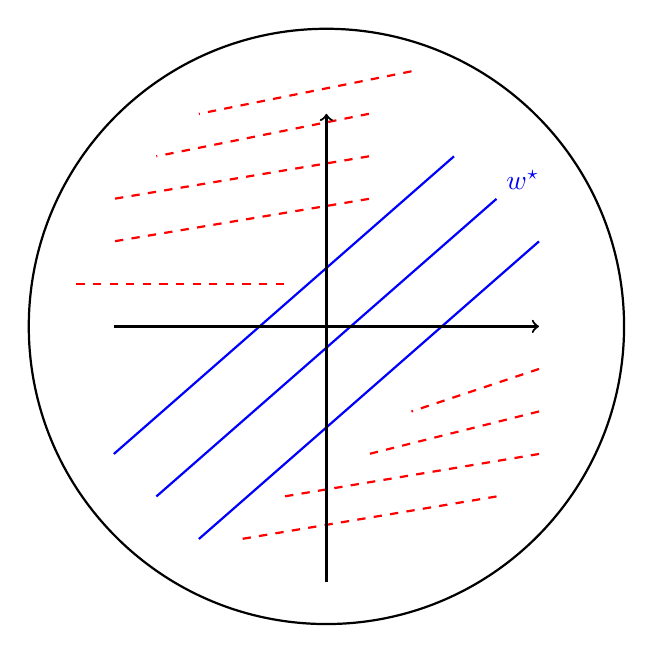
\begin{tikzpicture} [scale = 1] 
\draw[red, dashed, thick] (7.56, 2.44) -- (4.32, 1.9);
\draw[red, dashed, thick] (8.1, 2.98) -- (4.86, 2.44);
\draw[red, dashed, thick] (8.1, 3.52) -- (5.94, 2.98);
\draw[red, dashed, thick] (8.1, 4.06) -- (6.48, 3.52);
\draw[red, dashed, thick] (4.86, 5.14) -- (2.16, 5.14);
\draw[red, dashed, thick] (5.94, 6.22) -- (2.7, 5.68);
\draw[red, dashed, thick] (5.94, 6.76) -- (2.7, 6.22);
\draw[red, dashed, thick] (5.94, 7.3) -- (3.24, 6.76);
\draw[red, dashed, thick] (6.48, 7.84) -- (3.78, 7.3);
\node[blue, above right] at (7.56, 6.22){$w^\star $};
\draw[blue, thick] (3.78, 1.9) -- (8.1, 5.68);
\draw[blue, thick] (2.7, 2.98) -- (7.02, 6.76);
\draw[blue, thick] (3.24, 2.44) -- (7.56, 6.22);
\draw[black, ->, thick] (5.4, 1.36) -- (5.4, 7.3);
\draw[black, ->, thick] (2.7, 4.6) -- (8.1, 4.6);
\draw[black, thick] (5.4, 4.6) ellipse (3.78 and 3.78);
\end{tikzpicture} 
\end{figure}
\begin{align*}
S  &= \left\{\left(x_{1}, y_{1}\right), ..., \left(x_{n}, y_{n}\right)\right\}
\\ &s  \in \displaystyle\bigcup _{T=1}^{\infty} S^{T}
\end{align*}
\begin{align*}
&X , Y  \in \left\{-1, 1\right\}
\\ &s  \in \displaystyle\bigcup _{T=1}^{\infty} \left(X \times Y\right)^{T}
\end{align*}
Interaction protocol:
\\* $\boxed{0}$ world picks $s $
\\* At time $t: $
\\* $\boxed{1}$ wrold shows $x_{t}$ in $S $
\\* $\boxed{2}$ learner predict $\hat{y}_{t} \in Y $
\\* $\boxed{3}$ world reveals $y_{t}$ in $S $ (learner "learns, updates")
\newline \newline
ADD Realizability assumption: $\mathcal{H}$
\begin{align*}
\exists h^\star  \in \mathcal{H} : \;\forall\; s_{x} \in \displaystyle\bigcup _{T=1}^{\infty} X^{T} , \;\forall\; x_{t} \in s_{x} , y_{t} &= h^\star \left(x_{t}\right)
\end{align*}
Special case: $\left|  \mathcal{H}  \right| < \infty$
\\* Version space
\begin{align*}
VS  :&= \left\{h \in \mathcal{H} : h  \text{\;is consistent with all data so far\;}\right\}
\end{align*}



\section{Lecture $15$} 
Online learning:
\\* $\to $ realizable assumption: mistake bound
\\* $\to $ randomization: regret
\newline \newline
Given $\mathcal{H}, \exists h^\star  \in \mathcal{H}$ in each iteration $t $: world chooses $x_{t} \in X $ (not necessarily iid), learner predicts $\hat{y}_{t} \in Y $, world rewards $y_{t} := h^\star \left(x_{t}\right)$, learner incurs error $\mathbbm{1}_{\left(\hat{y}_{t} \neq  y_{t}\right)}$, "learns"
\newline \newline
Given sequence $S  = x_{1}, ..., x_{n}$, alg $A $, define the number of mistakes $A $ makes on $S $ by $M_{A}\left(S\right)$
\\* If $\exists A: \displaystyle\max_{S \in \displaystyle\bigcup _{n=0}^{\infty} X^{n}} M_{A}\left(S\right)$ is finite (mistake bound), then $\mathcal{H}$ is online-learnable.
\\* Also, what'$s \displaystyle\min_{A} \displaystyle\max_{S \in \displaystyle\bigcup _{n=0}^{\infty} X^{n}} M_{A}\left(S\right)$ ?
\newline \newline
"Baby steps" Assume $| \mathcal{H} | < \infty$
\\* $\exists A_{\text{\;consistent\;}}$ or $A_{\text{\;version space\;}}$, maintains a version space
\\* init: $VS_{0} = \mathcal{H}$
\\* At time $t $, pick any $h  \in VS_{t}$, predict $\hat{y}_{t} = h\left(x_{t}\right)$
\\* Update $VS_{t+1} = \left\{h' \in VS_{t} : h'\left(x_{t}\right) = y_{t}\right\}$
\newline \newline
\begin{align*}
X  &= \left\{x^{1}, ..., x^{m}\right\}
\\ h_{1} &= 1, 0, ..., 0
\\ h_{2} &= 0, 1, 0, ..., 0
\\ &...
\\ h_{m} &= 0, ..., 0, 1
\\ h_{m+1} &= h^\star  = 0, ..., 0
\\ M  &\leq  \left|  \mathcal{H}  \right| - 1
\end{align*}
\begin{align*}
&A_{\text{\;halving\;}}
\\ \hat{y}_{t} &= \arg\displaystyle\max_{y \in \left\{0, 1\right\}} \left|  \left\{h \in VS : h\left(x_{t}\right) = y\right\}  \right|
\\ 1 &\stackrel{h^\star  \in VS}{\leq} \left|  VS  \right| \leq  \dfrac{\left|  \mathcal{H}  \right|}{2^{M}} \Rightarrow  2^{M} \leq  \left|  \mathcal{H}  \right|, M \leq  \log_{2} \left|  \mathcal{H}  \right|
\end{align*}
$d  := \displaystyle\max_{S \in \displaystyle\bigcup _{n=0}^{\infty} X^{n}} M_{A}\left(S\right)$ (no longer assume $\left|  \mathcal{H}  \right| < \infty$) (still $\exists h^\star  \in \mathcal{H}$)
\\* Fix any $A $. Assume $\exists x \in X  \text{\;such that\;} \exists h_{1}, h_{2} \in \mathcal{H} \text{\;such that\;} h_{1}\left(x\right) \neq  h_{2}\left(x\right)$
\begin{align*}
h_{1}\left(x\right) &= 0
\\ h_{2}\left(x\right) &= 1
\end{align*}
\begin{figure}[H] \centering 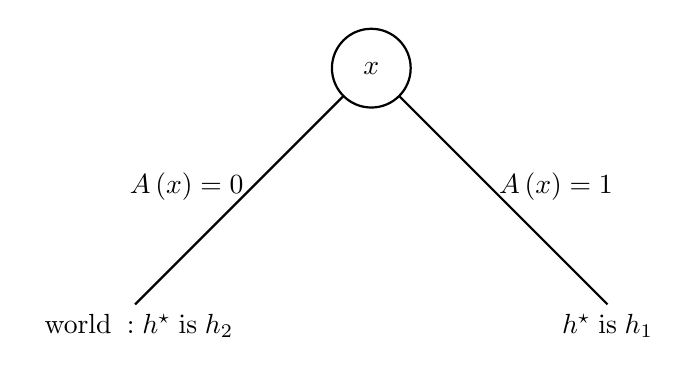
\begin{tikzpicture} [scale = 1] 
\draw[thick] (3.0, 3.0) -- (0.0, 0.0);
\draw[thick] (3.0, 3.0) -- (6.0, 0.0);
\draw[fill = white, thick] (3.0, 3.0) circle [radius = 0.5];
\node[] at (3.0, 3.0){$x $};
\node[left] at (1.5, 1.5){$A\left(x\right)  = 0$};
\node[right] at (4.5, 1.5){$A\left(x\right)  = 1$};
\node[below] at (0.0, 0.0){$\text{\;world\;}: h^\star  \text{\;is\;} h_{2}$};
\node[below] at (6.0, 0.0){$h^\star  \text{\;is\;} h_{1}$};
\end{tikzpicture} 
\end{figure}
World wants
\begin{align*}
&\mathcal{H} \text{\;such that\;} \exists
\end{align*}
\begin{figure}[H] \centering \begin{tikzpicture} [scale = 1] 
\draw[thick] (6.0, 6.0) -- (3.0, 3.0);
\draw[thick] (6.0, 6.0) -- (9.0, 3.0);
\draw[thick] (3.0, 3.0) -- (0.0, 0.0);
\draw[thick] (3.0, 3.0) -- (5.0, 0.0);
\draw[thick] (9.0, 3.0) -- (7.0, 0.0);
\draw[thick] (9.0, 3.0) -- (12.0, 0.0);
\draw[fill = white, thick] (6.0, 6.0) circle [radius = 0.5];
\draw[fill = white, thick] (3.0, 3.0) circle [radius = 0.5];
\draw[fill = white, thick] (9.0, 3.0) circle [radius = 0.5];
\node[] at (6.0, 6.0){$x_{1}$};
\node[] at (3.0, 3.0){$x_{2}$};
\node[] at (9.0, 3.0){$x_{3}$};
\node[left] at (4.5, 4.5){$0$};
\node[right] at (7.5, 4.5){$1$};
\node[left] at (1.5, 1.5){$0$};
\node[right] at (4.0, 1.5){$1$};
\node[left] at (8.0, 1.5){$1$};
\node[right] at (10.5, 1.5){$1$};
\node[below] at (0.0, 0.0){$h_{1}\left(x_{1}\right) = 0$};
\node[below] at (0.0, -0.5){$h_{1}\left(x_{2}\right) = 0$};
\node[below] at (5.0, 0.0){$h_{2}\left(x_{1}\right) = 0$};
\node[below] at (5.0, -0.5){$h_{2}\left(x_{2}\right) = 1$};
\node[below] at (7.0, 0.0){$h_{3}\left(x_{1}\right) = 1$};
\node[below] at (7.0, -0.5){$h_{3}\left(x_{2}\right) = 0$};
\node[below] at (12.0, 0.0){$h_{4}\left(x_{1}\right) = 1$};
\node[below] at (12.0, -0.5){$h_{4}\left(x_{2}\right) = 1$};
\end{tikzpicture} 
\end{figure}
World asks $\mathcal{H}$ "is there a tree with $h $ at the leaves?"
\newline \newline
\begin{center} \begin{tabular}{|c|c|c|c|c|c|}
\hline
 . &$x_{1}$ &$x_{2}$ &$x_{3}$ &$...$\\ \hline
$h_{1}$ &$0$ &$0$ &$^\star $ &\\ \hline
$h_{2}$ &$0$ &$1$ &$^\star $ &\\ \hline
$h_{3}$ &$1$ &$^\star $ &$0$ &\\ \hline
$h_{4}$ &$1$ &$^\star $ &$1$ &\\ \hline
$...$ & & & &\\ \hline
\end{tabular} \end{center}
\begin{figure}[H] \centering \begin{tikzpicture} [scale = 1] 
\draw[thick] (3.0, 3.0) -- (0.0, 0.0);
\draw[thick] (3.0, 3.0) -- (6.0, 0.0);
\draw[fill = white, thick] (3.0, 3.0) circle [radius = 0.5];
\node[] at (3.0, 3.0){$x_{1}$};
\node[left] at (1.5, 1.5){$0$};
\node[right] at (4.5, 1.5){$1$};
\node[below] at (0.0, 0.0){$h_{2}$};
\node[below] at (6.0, 0.0){$h_{1}$};
 
\draw[thick] (11.0, 3.0) -- (8.0, 0.0);
\draw[thick] (11.0, 3.0) -- (14.0, 0.0);
\draw[fill = white, thick] (11.0, 3.0) circle [radius = 0.5];
\node[] at (11.0, 3.0){$x_{n}$};
\node[left] at (9.5, 1.5){$0$};
\node[right] at (12.5, 1.5){$1$};
\node[below] at (8.0, 0.0){$h_{1}$};
\node[below] at (14.0, 0.0){$h_{n}$};
\end{tikzpicture} 
\end{figure}
\begin{align*}
\mathcal{H} &= \left\{h_{i} , i \in \left[n\right]\right\}
\\ h_{i}^{^\star } &= \mathbbm{1}_{\left(x = x_{i}\right)} \;\forall\; i \in \left[n \right]
\\ \mathcal{H}^{2} &= \mathcal{H} \cup \left\{h_{+} : h_{+} \left(x\right) = 1, \;\forall\; x\right\}
\end{align*}
\begin{figure}[H] \centering \begin{tikzpicture} [scale = 1] 
\draw[thick] (6.0, 6.0) -- (3.0, 3.0);
\draw[thick] (6.0, 6.0) -- (9.0, 3.0);
\draw[thick] (3.0, 3.0) -- (0.0, 0.0);
\draw[thick] (3.0, 3.0) -- (5.0, 0.0);
\draw[thick] (9.0, 3.0) -- (7.0, 0.0);
\draw[thick] (9.0, 3.0) -- (12.0, 0.0);
\draw[fill = white, thick] (6.0, 6.0) circle [radius = 0.5];
\draw[fill = white, thick] (3.0, 3.0) circle [radius = 0.5];
\draw[fill = white, thick] (9.0, 3.0) circle [radius = 0.5];
\node[] at (6.0, 6.0){$x_{1}$};
\node[] at (3.0, 3.0){$x_{2}$};
\node[] at (9.0, 3.0){$x_{3}$};
\node[left] at (4.5, 4.5){$0$};
\node[right] at (7.5, 4.5){$1$};
\node[left] at (1.5, 1.5){$0$};
\node[right] at (4.0, 1.5){$1$};
\node[left] at (8.0, 1.5){$1$};
\node[right] at (10.5, 1.5){$1$};
\node[below] at (0.0, 0.0){$h_{4}$};
\node[below] at (5.0, 0.0){$h_{2}$};
\node[below] at (7.0, 0.0){$h_{3}$};
\node[below] at (12.0, 0.0){$h_{+}$};
\end{tikzpicture} 
\end{figure}
\begin{figure}[H] \centering \begin{tikzpicture} [scale = 1] 
\draw[thick] (6.0, 6.0) -- (3.0, 3.0);
\draw[thick] (6.0, 6.0) -- (9.0, 3.0);
\draw[thick] (3.0, 3.0) -- (0.0, 0.0);
\draw[thick] (3.0, 3.0) -- (5.0, 0.0);
\draw[thick] (9.0, 3.0) -- (7.0, 0.0);
\draw[thick] (9.0, 3.0) -- (12.0, 0.0);
\draw[fill = white, thick] (6.0, 6.0) circle [radius = 0.5];
\draw[fill = white, thick] (3.0, 3.0) circle [radius = 0.5];
\draw[fill = white, thick] (9.0, 3.0) circle [radius = 0.5];
\node[] at (6.0, 6.0){$x_{1}$};
\node[] at (3.0, 3.0){$x_{2}$};
\node[] at (9.0, 3.0){$x_{2}$};
\node[left] at (4.5, 4.5){$0$};
\node[right] at (7.5, 4.5){$1$};
\node[left] at (1.5, 1.5){$0$};
\node[right] at (4.0, 1.5){$1$};
\node[left] at (8.0, 1.5){$1$};
\node[right] at (10.5, 1.5){$1$};
\node[below] at (0.0, 0.0){$h_{4}$};
\node[below] at (5.0, 0.0){$h_{2}$};
\node[below] at (7.0, 0.0){$h_{1}$};
\node[below] at (12.0, 0.0){$h_{+}$};
\end{tikzpicture} 
\end{figure}
What is the deepest complete tree with $h $ at the leaves?
\\* depth $=$ Littlestone dimension of $\mathcal{H}$.
\newline \newline



\section{Lecture $16$} 
Realizable online learning
\begin{align*}
\displaystyle\max_{A} \displaystyle\max_{h^\star  \in \mathcal{H}} \displaystyle\max_{s \in \displaystyle\bigcup _{n=0}^{\infty} X^{n}} M_{A}\left(S\right) &\geq  \text{\;depth of "that tree"\;} := Ldim\left(\mathcal{H}\right) 
\end{align*}
Given $X , \mathcal{H}$, find the deepest complete tree of the form
\begin{figure}[H] \centering \begin{tikzpicture} [scale = 1] 
\draw[thick] (6.0, 6.0) -- (3.0, 3.0);
\draw[thick] (6.0, 6.0) -- (9.0, 3.0);
\draw[thick] (3.0, 3.0) -- (0.0, 0.0);
\draw[thick] (3.0, 3.0) -- (4.0, 0.0);
\draw[thick] (9.0, 3.0) -- (8.0, 0.0);
\draw[thick] (9.0, 3.0) -- (12.0, 0.0);
\draw[thick] (0.0, 0.0) -- (-1.0, -3.0);
\draw[thick] (0.0, 0.0) -- (1.0, -3.0);
\draw[thick] (4.0, 0.0) -- (3.0, -3.0);
\draw[thick] (4.0, 0.0) -- (5.0, -3.0);
\draw[thick] (8.0, 0.0) -- (7.0, -3.0);
\draw[thick] (8.0, 0.0) -- (9.0, -3.0);
\draw[thick] (12.0, 0.0) -- (11.0, -3.0);
\draw[thick] (12.0, 0.0) -- (13.0, -3.0);
\draw[fill = white, thick] (6.0, 6.0) circle [radius = 0.5];
\draw[fill = white, thick] (3.0, 3.0) circle [radius = 0.5];
\draw[fill = white, thick] (9.0, 3.0) circle [radius = 0.5];
\draw[fill = white, thick] (0.0, 0.0) circle [radius = 0.5];
\draw[fill = white, thick] (4.0, 0.0) circle [radius = 0.5];
\draw[fill = white, thick] (8.0, 0.0) circle [radius = 0.5];
\draw[fill = white, thick] (12.0, 0.0) circle [radius = 0.5];
\node[] at (6.0, 6.0){$x_{1}$};
\node[] at (3.0, 3.0){$x_{2}$};
\node[] at (9.0, 3.0){$x_{3}$};
\node[] at (0.0, 0.0){$x_{4}$};
\node[left] at (4.5, 4.5){$0$};
\node[right] at (7.5, 4.5){$1$};
\node[left] at (1.5, 1.5){$0$};
\node[right] at (3.5, 1.5){$1$};
\node[left] at (8.5, 1.5){$0$};
\node[right] at (10.5, 1.5){$1$};
\node[left] at (-0.5, -1.5){$0$};
\node[right] at (0.5, -1.5){$1$};
\node[below] at (-1.0, -3.0){$\exists h \in \mathcal{H}$};
\end{tikzpicture} 
\end{figure}
Ex. Suppose $VC\left(\mathcal{H}\right)  = d. $
\\* What about $Ldim\left(HsC\right) $?
\\* $\exists x_{1} ... x_{d}$ shattered by $\mathcal{H}$.
\newline \newline
\begin{figure}[H] \centering \begin{tikzpicture} [scale = 1] 
\draw[thick] (6.0, 6.0) -- (3.0, 3.0);
\draw[thick] (6.0, 6.0) -- (9.0, 3.0);
\draw[thick] (3.0, 3.0) -- (0.0, 0.0);
\draw[thick] (3.0, 3.0) -- (4.0, 0.0);
\draw[thick] (9.0, 3.0) -- (8.0, 0.0);
\draw[thick] (9.0, 3.0) -- (12.0, 0.0);
\draw[thick] (0.0, 0.0) -- (-1.0, -3.0);
\draw[dashed, thick] (0.0, 0.0) -- (1.0, -3.0);
\draw[dashed, thick] (12.0, 0.0) -- (13.0, -3.0);
\draw[thick] (-1.0, -3.0) -- (-1.5, -6.0);
\draw[thick] (-1.0, -3.0) -- (0.5, -6.0);
\draw[thick] (13.0, -3.0) -- (11.5, -6.0);
\draw[thick] (13.0, -3.0) -- (13.5, -6.0);
\draw[fill = white, thick] (6.0, 6.0) circle [radius = 0.5];
\draw[fill = white, thick] (3.0, 3.0) circle [radius = 0.5];
\draw[fill = white, thick] (9.0, 3.0) circle [radius = 0.5];
\draw[fill = white, thick] (0.0, 0.0) circle [radius = 0.5];
\draw[fill = white, thick] (4.0, 0.0) circle [radius = 0.5];
\draw[fill = white, thick] (8.0, 0.0) circle [radius = 0.5];
\draw[fill = white, thick] (12.0, 0.0) circle [radius = 0.5];
\draw[fill = white, thick] (-1.0, -3.0) circle [radius = 0.5];
\draw[fill = white, thick] (13.0, -3.0) circle [radius = 0.5];
\draw[fill = white, thick] (-1.5, -6.0) circle [radius = 0.5];
\draw[fill = white, thick] (0.5, -6.0) circle [radius = 0.5];
\draw[fill = white, thick] (13.5, -6.0) circle [radius = 0.5];
\node[] at (6.0, 6.0){$x_{1}$};
\node[] at (3.0, 3.0){$x_{2}$};
\node[] at (9.0, 3.0){$x_{2}$};
\node[] at (0.0, 0.0){$x_{3}$};
\node[] at (4.0, 0.0){$x_{3}$};
\node[] at (8.0, 0.0){$x_{3}$};
\node[] at (12.0, 0.0){$x_{3}$};
\node[] at (-1.0, -3.0){$x_{d}$};
\node[] at (12.0, -3.0){$x_{d}$};
\node[] at (-1.5, -6.0){$\exists h_{1}$};
\node[] at (0.5, -6.0){$h_{2}$};
\node[] at (13.5, -6.0){$h_{2^{d}}$};
\end{tikzpicture} 
\end{figure}
\begin{thm} \label{thm:ldim} 
$Ldim\left(\mathcal{H}\right)  \geq  VC\left(\mathcal{H}\right) $
\newline \newline\end{thm}
Ex: "One-hot" $\left\{h_{x} : x \in C\right\} := \mathcal{H}$
\\* $Ldim\left(\mathcal{H}\right)  = 1$ possibly $| \mathcal{H} | = \infty$
\\* Ex: $\mathcal{H} = \left\{h_{a}, a \in \left[0, 1\right]: h_{a}\left(x\right) = \mathbbm{1}_{\left(x \geq  a\right)}\right\}$,
\begin{align*}
VC\left(\mathcal{H}\right)  &= 1
\\ Ldim\left(\mathcal{H}\right)  &= \infty
\end{align*}
\begin{figure}[H] \centering 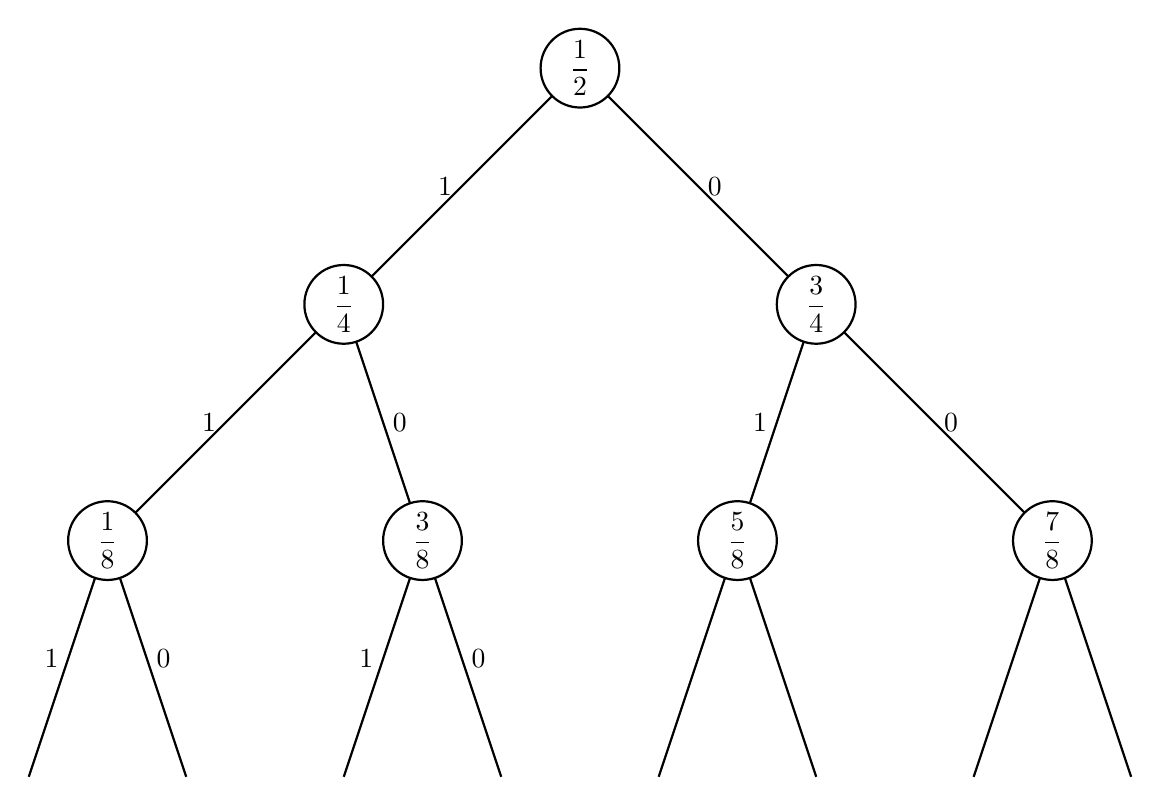
\begin{tikzpicture} [scale = 1] 
\draw[thick] (6.0, 6.0) -- (3.0, 3.0);
\draw[thick] (6.0, 6.0) -- (9.0, 3.0);
\draw[thick] (3.0, 3.0) -- (0.0, 0.0);
\draw[thick] (3.0, 3.0) -- (4.0, 0.0);
\draw[thick] (9.0, 3.0) -- (8.0, 0.0);
\draw[thick] (9.0, 3.0) -- (12.0, 0.0);
\draw[thick] (0.0, 0.0) -- (-1.0, -3.0);
\draw[thick] (0.0, 0.0) -- (1.0, -3.0);
\draw[thick] (4.0, 0.0) -- (3.0, -3.0);
\draw[thick] (4.0, 0.0) -- (5.0, -3.0);
\draw[thick] (8.0, 0.0) -- (7.0, -3.0);
\draw[thick] (8.0, 0.0) -- (9.0, -3.0);
\draw[thick] (12.0, 0.0) -- (11.0, -3.0);
\draw[thick] (12.0, 0.0) -- (13.0, -3.0);
\draw[fill = white, thick] (6.0, 6.0) circle [radius = 0.5];
\draw[fill = white, thick] (3.0, 3.0) circle [radius = 0.5];
\draw[fill = white, thick] (9.0, 3.0) circle [radius = 0.5];
\draw[fill = white, thick] (0.0, 0.0) circle [radius = 0.5];
\draw[fill = white, thick] (4.0, 0.0) circle [radius = 0.5];
\draw[fill = white, thick] (8.0, 0.0) circle [radius = 0.5];
\draw[fill = white, thick] (12.0, 0.0) circle [radius = 0.5];
\node[] at (6.0, 6.0){$\dfrac{1}{2}$};
\node[] at (3.0, 3.0){$\dfrac{1}{4}$};
\node[] at (9.0, 3.0){$\dfrac{3}{4}$};
\node[] at (0.0, 0.0){$\dfrac{1}{8}$};
\node[] at (4.0, 0.0){$\dfrac{3}{8}$};
\node[] at (8.0, 0.0){$\dfrac{5}{8}$};
\node[] at (12.0, 0.0){$\dfrac{7}{8}$};
\node[left] at (4.5, 4.5){$1$};
\node[right] at (7.5, 4.5){$0$};
\node[left] at (1.5, 1.5){$1$};
\node[right] at (3.5, 1.5){$0$};
\node[left] at (8.5, 1.5){$1$};
\node[right] at (10.5, 1.5){$0$};
\node[left] at (-0.5, -1.5){$1$};
\node[right] at (0.5, -1.5){$0$};
\node[left] at (3.5, -1.5){$1$};
\node[right] at (4.5, -1.5){$0$};
\end{tikzpicture} 
\end{figure}
\begin{figure}[H] \centering \begin{tikzpicture} [scale = 1] 
\draw[thick] (0.0, 0.0) -- (6.0, 0.0);
\node[] at (2.0, 0.0){x};
\node[] at (4.0, 0.0){x};
\draw[blue, thick] (1.0, 1.5) -- (1.0, -1.5);
\draw[blue, ->, thick] (1.0, 1.0) -- (2.0, 1.0);
\node[below] at (0.0, -0.1){$0$};
\node[below] at (6.0, -0.1){$1$};
\node[below] at (2.0, -0.1){$1$};
\node[below] at (4.0, -0.1){$1$};
\node[below] at (2.0, -0.6){$0$};
\node[below] at (4.0, -0.6){$1$};
\node[below] at (2.0, -1.1){$0$};
\node[below] at (4.0, -1.1){$0$};
\draw[fill = black, thick] (0.0, 0.0) circle [radius = 0.1];
\draw[fill = black, thick] (6.0, 0.0) circle [radius = 0.1];
\end{tikzpicture} 
\end{figure}
Standard Optimal Alg: $A_{\text{\;SOA\;}}$
\\* receive $x_{t}$
\begin{align*}
VS^{0}  \cup VS^{1} , VS^{p}  &= \left\{h \in VS : h\left(x_{t}\right) = p \right\}
\\ \hat{y}_{t} &= \arg\displaystyle\max_{p \in Y} Ldim  \left(VS^{p} \right)
\end{align*}
receive $y_{t}$
\begin{align*}
VS  &\leftarrow VS^{y_{t}} 
\end{align*}
\begin{figure}[H] \centering 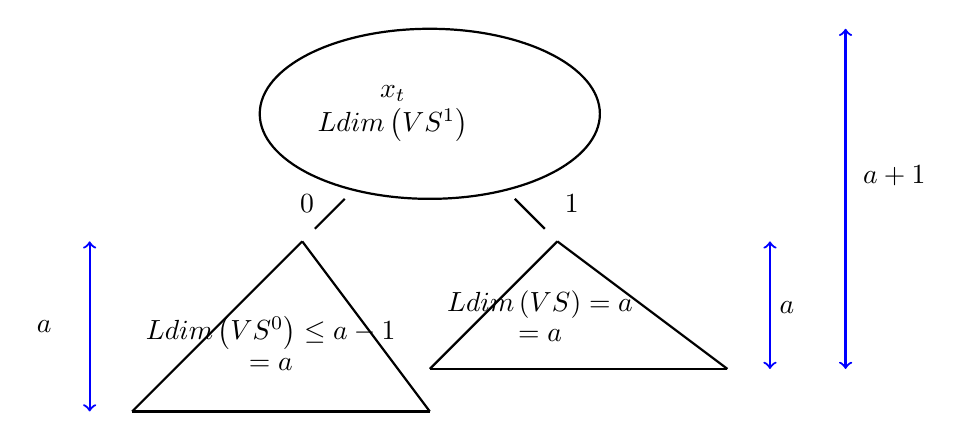
\begin{tikzpicture} [scale = 1] 
\node[black, right] at (9.72, 3.76){$a $};
\node[black, right] at (10.78, 5.44){$a  + 1$};
\node[black, left] at (0.72, 3.52){$a $};
\node[black] at (4.93, 6.08){$Ldim\left(VS^{1} \right) $};
\node[black] at (4.93, 6.48){$x_{t}$};
\node[black] at (6.8, 3.4){$= a $};
\node[black] at (6.8, 3.8){$Ldim\left(VS \right)  = a $};
\node[black] at (3.38, 3.04){$= a $};
\node[black] at (3.38, 3.44){$Ldim\left(VS^{0} \right)  \leq  a - 1$};
\node[black, right] at (6.99, 5.08){$1$};
\node[black, right] at (3.63, 5.08){$0$};
\draw[blue, <->, thick] (10.68, 7.3) -- (10.68, 2.98);
\draw[blue, <->, thick] (9.72, 4.6) -- (9.72, 2.98);
\draw[blue, <->, thick] (1.08, 4.6) -- (1.08, 2.44);
\draw[black, thick] (5.4, 2.98) -- (7.02, 4.6);
\draw[black, thick] (7.02, 4.6) -- (9.18, 2.98);
\draw[black, thick] (5.4, 2.98) -- (9.18, 2.98);
\draw[black, thick] (3.78, 4.6) -- (5.4, 2.44);
\draw[black, thick] (1.62, 2.44) -- (5.4, 2.44);
\draw[black, thick] (3.78, 4.6) -- (1.62, 2.44);
\draw[black, thick] (6.48, 5.14) -- (6.86, 4.76);
\draw[black, thick] (4.32, 5.14) -- (3.94, 4.76);
\draw[black, thick] (5.4, 6.22) ellipse (2.16 and 1.08);
\end{tikzpicture} 
\end{figure}
World: $x_{t}$
\\* Alg: predicts: $\hat{y}_{t}$
\\* World: give $y_{t} \in Y $
\newline \newline
\begin{align*}
\text{\;regret\;} : \displaystyle\sum_{t=1}^{T} \ell\left(\hat{y}_{t}\left(x_{t}\right), y_{t}\right) - \displaystyle\min_{h \in \mathcal{H}} \displaystyle\sum_{t=1}^{T} \ell\left(h\left(x_{t}\right), y_{t}\right) &\geq _{\text{\;Show this!\;}} \dfrac{T}{2}
\end{align*}



\section{Lecture $17$} 
No longer assume $\exists h^\star  \in \mathcal{H} \text{\;such that\;} y_{t} = h^\star \left(x_{t}\right)$
\\* (expected) regret wrt $\mathcal{H}$ (want: $o\left(T\right) $, in fact $\sqrt{T}$)
\begin{align*}
&\displaystyle\sup_{\left(x, y\right)_{1:T}} \mathbb{E} \displaystyle\sum_{t=1}^{T} \mathbbm{1}_{\left(\underbrace{\hat{y}_{t}\left(x_{t}\right)}_{\text{\;made by\;} A} \neq  y_{t}\right)} - \displaystyle\min_{h \in \mathcal{H}} \displaystyle\sum_{t=1}^{T} \mathbbm{1}_{\left(h\left(x_{t}\right) \neq  y_{t}\right)}
\end{align*}
Ex: $\mathcal{H} = \left\{h_{0}, h_{1}\right\}, A $ deterministic, regret $\geq  \dfrac{T}{2}$
\\* $A $ randomized
\newline \newline

\subsection{Weighted Majority}
(learn from expert advise)
\\* Given $d $ experts, horizon $T $, stepsize $\eta > 0$
\begin{enumerate}
\item init $\tilde{w}^{\left(1\right)} = \underbrace{\left(1, ..., 1\right)}_{d}$ (unnormalized weights)
\item For $t  = 1, 2, ..., T $
\item $w^{\left(t\right)} = \dfrac{\tilde{w}^{\left(t\right)}}{Z_{t}}$ where $Z_{t} = \displaystyle\sum_{i=1}^{d} \tilde{w}_{i}^{\left(t\right)}$
\item Choose expert $i  \sim  w^{\left(t\right)}$
\item Observe loss vector $V_{t} = \left(v_{t_{1}} , ..., \overbrace{\boxed{v_{t_{i}}}}^{MAB} , ..., t_{t_{d}}\right) \in \left[0, 1\right]^{d}$ "bounded", pay expected loss $w^{\left(t\right)^{T}} V_{t}$
\item update $\tilde{w}_{j}^{\left(t+1\right)} = \tilde{w}_{j}^{\left(t\right)} e^{- \eta v_{t_{j}}} \;\forall\; j \in \left[d\right]$
\end{enumerate}

\begin{align*}
\left(\displaystyle\sum_{t=1}^{T} w^{\left(t\right)^{T}} V_{t}\right) - \displaystyle\min_{j \in \left[d\right]} \displaystyle\sum_{t=1}^{T} V_{t_{j}} &\leq  \sqrt{2 \left(\log d\right) T}
\end{align*}
Proof:
\begin{align*}
\log \dfrac{Z_{t+1}}{Z_{t}} &= \log \dfrac{\displaystyle\sum_{j=1}^{d} \tilde{w}_{j}^{\left(t\right)} e^{- \eta V_{t_{j}}}}{Z_{t}}
\\ &= \log \displaystyle\sum_{j}^{d} w_{j}^{\left(t\right)} e^{-\eta V_{t_{j}}}
\\ &\leq  \log \displaystyle\sum_{j} w_{j}^{\left(t\right)} \left[1 - \eta V_{t_{j}} + \dfrac{\eta^{2} V_{t_{j}}^{2}}{2}\right]
\\ &= \log \left[1 - \underbrace{\displaystyle\sum_{j} w_{j}^{\left(t\right)} \left(\eta V_{t_{j}} - \dfrac{\eta^{2} V_{t_{j}}^{2}}{2}\right)}_{:= b \in \left(0, 1\right)}\right]
\\ &\leq  \log e^{-b}
\\ &= - \eta \left(w^{\left(t\right)^{T}} V_{t}\right) + \eta^{2} \displaystyle\sum_{j} w_{j}^{\left(t\right)} \dfrac{V_{t_{j}}^{2}}{2}
\\ &\leq  - \eta w^{\left(t\right)^{T}} V_{t} + \dfrac{\eta^{2}}{2}
\end{align*}
\begin{figure}[H] \centering \begin{tikzpicture} [scale = 1] 
\node[black, right] at (8.25, 2.92){$a $};
\node[black, right] at (6.63, 2.92){$1$};
\node[black, right] at (3.75, 3.04){$0$};
\draw[black, thick] (4.32, 5.68).. controls(4.91, 4.85)and(5.71, 4.41)..(6.73, 4.36);
\draw[black, thick] (4.32, 5.68) -- (6.63, 5.69);
\draw[black, fill = black, thick] (6.56, 3.48) circle [radius = 0.04];
\draw[black, ->, thick] (1.62, 3.52) -- (8.1, 3.52);
\draw[black, ->, thick] (4.32, 2.44) -- (4.32, 7.84);
\end{tikzpicture} 
\end{figure}
\begin{align*}
&a  \in \left(0, 1\right)
\\ e^{-a} &\leq  1 - a + \dfrac{a^{2}}{2}
\end{align*}
\begin{figure}[H] \centering \begin{tikzpicture} [scale = 1] 
\node[blue, right] at (7.78, 1.18){$1 - x $};
\node[blue, right] at (5.57, 6.7){$e^{-x}$};
\draw[blue, thick] (3.24, 8.38).. controls(3.71, 5.26)and(5.39, 3.66)..(8.25, 3.58);
\draw[blue, thick] (2.16, 7.3) -- (8.1, 1.9);
\draw[black, thick] (4.86, 8.38) -- (4.86, 1.9);
\draw[black, thick] (1.62, 2.98) -- (8.64, 2.98);
\end{tikzpicture} 
\end{figure}
\begin{align*}
1 - x &\leq  e^{-x}
\end{align*}




\section{Lecture $18$} 

\subsection{Online learning}
(no assumption on $\exists h^\star  \in \mathcal{H}, y_{t} = h^\star \left(x_{t}\right)$)
\begin{itemize}
\item subroutine: wighted Majority
\end{itemize}Input: $d  = \#$ experts, $T $ rounds
\\* init $\tilde{w}^{\left(1\right)} = \left(1, ..., 1\right)_{d}$
\\* for $t  = 1, 2, ...$
\begin{align*}
Z_{t} &= \tilde{w}^{\left(t\right)^{T}} 1, w^{\left(t\right)} = \dfrac{\tilde{w}^{\left(t\right)}}{Z_{t}}
\end{align*}
pick $i  \sim  w^{\left(t\right)}$ to predict
\\* suffer expected loss $w^{\left(t\right)^{T}} V^{\left(t\right)}$
\begin{align*}
\tilde{w}^{\left(t + 1\right)} &= \tilde{w}^{\left(t\right)} e^{-\eta V_{i}^{\left(t\right)}} \;\forall\; i = 1 ... d 
\end{align*}
\begin{align*}
V_{i}^{\left(t\right)} :&= \ell\left(\overbrace{\text{\;expert\;} _{i}\left(x_{t}\right)}^{h_{i}\left(x_{t}\right)} , y_{t}\right)
\\ V^{\left(t\right)} :&= \begin{bmatrix} V_{1}^{\left(t\right)} \\ ... \\ V_{d}^{\left(t\right)} \end{bmatrix} \in \left[0, 1\right]^{d}
\end{align*}
\begin{thm} \label{thm:wmj} 
$\left(\displaystyle\sum_{t=1}^{T} w^{\left(t\right)^{T}} V^{\left(t\right)}\right) - \left(\underbrace{\displaystyle\min_{i \in \left[d\right]}}_{\text{\;"best expert"\;}} \displaystyle\sum_{t=1}^{T} V_{i}^{\left(t\right)}\right)$
\newline \newline\end{thm}
\begin{align*}
\log \dfrac{Z_{t+1}}{Z_{t}} &= \log \displaystyle\sum_{i}^{d} w_{i}^{\left(t\right)} e^{- \eta V_{i}^{\left(t\right)}}
\\ &\stackrel{\left[e^{-x} \leq  1 - x + \dfrac{x^{2}}{2}\right]}{\leq} \log\left[\displaystyle\sum_{i}^{d} w_{i}^{\left(t\right)} \left[1 - \eta V_{i}^{\left(t\right)} + \dfrac{\eta^{2} V_{i}^{\left(t\right)^{2}}}{2}\right]\right]
\\ &= \log\left[1 - \displaystyle\sum_{i} w_{i}^{\left(t\right)} \left(\eta V_{i}^{\left(t\right)} - \dfrac{\eta^{2} V_{i}^{\left(t\right)^{2}}}{2}\right)\right]
\\ &\stackrel{1 - x \leq  e^{-x}}{\leq} \log e^{-\displaystyle\sum_{i} w_{i}^{\left(t\right)} \left(\eta V_{i}^{\left(t\right)} - \dfrac{\eta^{2} V_{i}^{\left(t\right)^{2}}}{2}\right)}
\\ &= -\eta w^{\left(t\right)^{T}} V^{\left(t\right)} + \displaystyle\sum_{i} w_{i}^{\left(t\right)} \dfrac{\eta^{2} V_{i}^{\left(t\right)^{2}}}{2}
\\ &\stackrel{V \in \left[0, 1\right]}{\leq} -\eta w^{\left(t\right)^{T}} V^{\left(t\right)} + \dfrac{\eta^{2}}{2} \leftarrow \boxed{1}
\end{align*}
Telescope $\boxed{1}$ over $t: $
\begin{align*}
\log Z_{T+1} - \log d &= \log Z_{T+1} - \log Z_{1}
\\ &= \displaystyle\sum_{t=1}^{T} \log \dfrac{Z_{t+1}}{Z_{t}}
\\ &\stackrel{\boxed{1}}{\leq} - \eta \displaystyle\sum_{t}^{T} w^{\left(t\right)^{T}} V^{\left(t\right)} + \dfrac{\eta^{2} T}{2} \leftarrow \boxed{2}
\end{align*}
\begin{align*}
Z_{T+1} &= \displaystyle\sum_{i} \tilde{w}_{i}^{\left(T + 1\right)}
\\ &= \displaystyle\sum_{i} 1 \cdot  e^{-\eta \displaystyle\sum_{t}^{T} V_{i}^{\left(t\right)}},
\\ \log Z_{T+1} &= \log \displaystyle\sum_{i}^{d} e^{-\eta \displaystyle\sum_{t}^{T} V_{i}^{\left(t\right)}}
\\ &\geq  \displaystyle\max_{i} \log e^{-\eta \displaystyle\sum_{t}^{T} V_{i}^{\left(t\right)}}
\\ &= \displaystyle\max_{i} - \eta \displaystyle\sum_{t}^{T} V_{i}^{\left(t\right)}
\\ &= - \eta \left(\displaystyle\min_{i} \displaystyle\sum_{t}^{T} V_{i}^{\left(t\right)}\right) \leftarrow \boxed{3}
\end{align*}
"best expert"
\newline \newline
\begin{align*}
\boxed{2} , \boxed{3} &\Rightarrow 
\\ -\eta \left(\displaystyle\min_{i} \displaystyle\sum_{t}^{T} V_{i}^{\left(t\right)}\right) - \log d &\stackrel{\boxed{3}}{\leq} \log Z_{T+1} - \log d
\\ &\leq  - \eta \displaystyle\sum_{t}^{T} w^{\left(t\right)^{T}} V^{\left(t\right)} + \dfrac{\eta^{2} T}{2}
\\ \displaystyle\sum_{t}^{T} w^{\left(t\right)^{T}} V_{i}^{\left(t\right)} - \displaystyle\min_{i \in \left[d\right]} \displaystyle\sum_{t}^{T} V_{i}^{\left(t\right)} &\leq  \dfrac{\log d}{\eta} + \dfrac{\eta T}{2} \to  \text{\;sublinear\;}
\end{align*}
\begin{align*}
&  \dfrac{\partial \text{\;RHS\;}}{\partial \eta} = 0
\\ &\Rightarrow  - \dfrac{\log d}{\eta^{2}} + \dfrac{T}{2} = 0
\\ &\Rightarrow  \dfrac{1}{\eta} = \sqrt{\dfrac{T}{2 \log d}}
\\ &\Rightarrow  \text{\;RHS\;} = \sqrt{2 T \log d }
\end{align*}
If $\left|  \mathcal{H}  \right| < \infty$
\begin{align*}
\text{\;regret\;} &\leq  \sqrt{2 T \log \left|  \mathcal{H}  \right|}
\end{align*}
when $\left|  \mathcal{H}  \right| = \infty$?
\newline \newline
\begin{itemize}
\item subroutine $2$
\end{itemize}SOA: $VS  = \mathcal{H}$
\\* for $t  = 1, 2, ...$
\\* receive $x_{t}$
\begin{align*}
&VS^{0}  \cup VS^{1} 
\\ \hat{y}_{t} &= \arg\displaystyle\max_{y} Ldim\left(VS^{y} \right) 
\\ VS  &\leftarrow VS^{y_{t}} 
\end{align*}
assuming $\exists h^\star  \in \mathcal{H}$
\\* s.t. $y_{t} = h^\star \left(x_{t}\right) \;\forall\; t $
\\* then SOA mistakes $\leq  Ldim\left(\mathcal{H}\right) $
\newline \newline
expert $\left(i_{1}, i_{2}, ..., i_{L}\right)$
\begin{align*}
1 &\leq  i_{1} < i_{2} < ... i_{L} \leq  T , L \leq  Ldim\left(\mathcal{H}\right)  < \infty
\end{align*}
init $VS  = \mathcal{H}$
\\* for $t  = 1, 2, ..., T $
\\* receive $x_{t}$
\\* $VS^{0}  = \left\{h \in VS , h\left(x_{t}\right) = 0\right\}$, same for $VS^{1} $
\\* if $t  \in \left\{i_{1}, ..., i_{L}\right\}$
\begin{align*}
\hat{y}_{t} &= \arg\displaystyle\min_{y} Ldim\left(VS^{y} \right)  \leftarrow \text{\;anti-SOA\;}
\end{align*}
else
\begin{align*}
\hat{y}_{t} &= \arg\displaystyle\max_{y} Ldim\left(VS^{y} \right)  \leftarrow \text{\;SOA\;}
\\ VS  &\leftarrow VS^{\hat{y}_{t}} 
\end{align*}
Given $x_{1} ... x_{T}$
\begin{align*}
&\;\forall\; h \in \mathcal{H}
\\ &\Rightarrow  h\left(x_{1}\right) ... h\left(x_{T}\right)
\end{align*}
want: $\exists L, i_{1} ... i_{L} s$.t. expert $\left(i_{1} ... i_{L}\right)$ produces the same predictions
\newline \newline
Run SOA on input
\begin{align*}
&x_{1}, h\left(x_{1}\right)
\\ &...
\\ &x_{T}, h\left(x_{T}\right)
\end{align*}
Lemma $21.13$
\newline \newline




\section{Lecture $19$} 

\subsection{Online Convex Optimization}
for $t  = 1, 2, ...$
\\* learner chooses $w^{\left(t\right)} \in$ Convex set $W $
\\* environment chooses loss function $f_{t} : W \to  \mathbb{R}$ convex (subgradient)
\\* learner suffers $f_{t}\left(w^{\left(t\right)}\right)$
\newline \newline
\begin{align*}
\text{\;regret\;} :&= \displaystyle\sum_{t=1}^{T} f_{t}\left(w^{\left(t\right)}\right) - \displaystyle\inf_{w \in W} \displaystyle\sum_{t=1}^{T} f_{t}\left(w\right)
\end{align*}
\begin{figure}[H] \centering \begin{tikzpicture} [scale = 1] 
\node[black, right] at (5.0, 1.0){$W $};
\node[black, right] at (1.53, 2.38){$0$};
\node[black, right] at (1.67, 7.24){$f $};
\node[blue, right] at (6.64, 1.78){$w^\star _{2}$};
\node[blue, right] at (3.46, 1.84){$w^\star _{1}$};
\node[blue, right] at (7.9, 4.48){$f_{2}$};
\node[blue, right] at (7.3, 7.78){$f_{1}$};
\draw[blue, thick] (3.78, 7.3).. controls(8.6, -0.64)and(6.21, 3.05)..(8.64, 4.06);
\draw[blue, thick] (2.16, 5.14).. controls(3.15, 3.29)and(3.65, -1.16)..(7.02, 7.3);
\draw[black, ->, thick] (2.16, 2.34) -- (8.1, 2.34);
\draw[black, ->, thick] (2.16, 1.9) -- (2.16, 6.76);
\end{tikzpicture} 
\end{figure}
Online gradient descent
\begin{align*}
w^{\left(1\right)} &= 0
\end{align*}
for $t  = 1, 2, ...$
\\* predict $w^{\left(t\right)}$
\\* receive $f_{t}\left(\cdot \right)$, suffer $f_{t}\left(w^{\left(t\right)}\right)$
\begin{align*}
w^{\left(t+1\right)} &= \text{\;Proj\;} _{W} \left[\underbrace{w^{\left(t\right)} - \underbrace{\eta}_{\text{\;stepsize\;}} \cdot  \underbrace{\partial}_{\text{\;subgradient\;}} f_{t}\left(w^{\left(t\right)}\right)}_{W^{\left(t + 1/2\right)}}\right]
\end{align*}
\begin{thm} \label{thm:t2115} 
(Thm $21.15$)
\begin{align*}
\text{\;Regret\;} &\leq  \displaystyle\inf_{w \in W} \dfrac{\left\|w\right\|^{2}}{2 \eta} + \dfrac{\eta}{2} \displaystyle\sum_{t=1}^{T} \left\|\partial f_{t}\left(w^{\left(t\right)}\right)\right\|^{2}
\\ \text{\;OR\;} \;\forall\; w \in W, \text{\;Regret\;} \left(w\right) &\leq  \dfrac{\left\|w\right\|^{2}}{2 \eta} + \dfrac{\eta}{2} \displaystyle\sum_{t=1}^{T} \left\|\partial f_{t}\left(w^{\left(t\right)}\right)\right\|^{2}
\end{align*}
\end{thm}
\begin{proof} \label{proof:t2115pf} 
Fix $w  \in W $
\begin{align*}
\left\|w^{\left(t+1\right)} - w\right\|^{2} - \left\|w^{\left(t\right)} - w\right\|^{2} &= \left(\left\|w^{t+1} - w\right\|^{2} - \left\|w^{t+1/2} - w\right\|^{2}\right) + \left(\left\|w^{t+1/2} - w\right\|^{2} - \left\|w^{t} - w\right\|^{2}\right)
\\ &\leq  0 + \left(\left\|w^{t} - \eta \partial f_{t}\left(w^{t}\right) - w\right\|^{2} - \left\|w^{t} - w\right\|^{2}\right)
\\ &= \left(-2 \left(w^{t} - w\right)^{T} \eta \partial f_{t}\left(w^{t}\right) + \eta^{2} \left\|\partial f_{t}\left(w^{t}\right)\right\|^{2}\right)
\\ &\leq  2 \eta \left(f_{t}\left(w^{t}\right) - f_{t}\left(w\right)\right) + \eta^{2} \left\|\partial f_{t}\left(w^{t}\right)\right\|^{2} \leftarrow \boxed{1}
\end{align*}\end{proof}
\begin{figure}[H] \centering 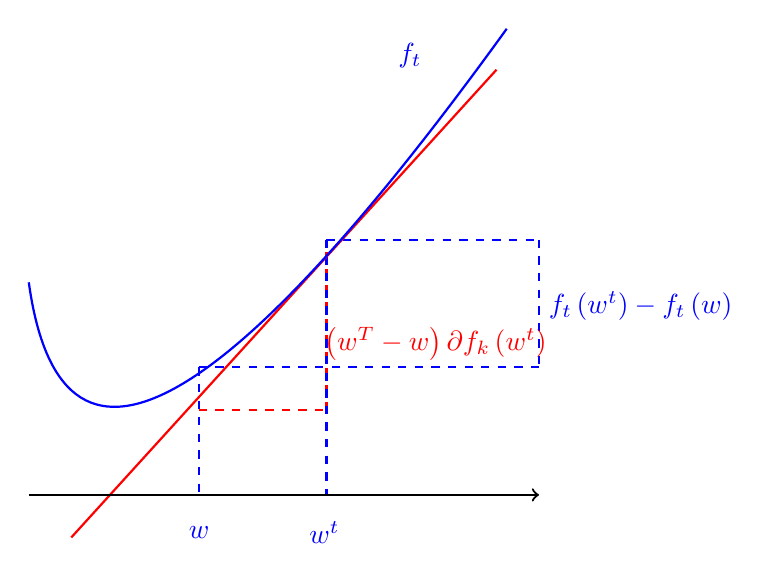
\begin{tikzpicture} [scale = 1] 
\draw[blue, dashed, thick] (8.1, 5.14) -- (8.1, 3.52);
\node[blue, right] at (6.19, 7.48){$f_{t}$};
\draw[red, dashed, thick] (5.4, 2.98) -- (5.4, 5.14);
\node[red, right] at (5.25, 3.82){$\left(w^{T} - w\right) \partial f_{k}\left(w^{t}\right)$};
\node[blue, right] at (8.1, 4.3){$f_{t}\left(w^{t}\right) - f_{t}\left(w\right)$};
\node[blue, right] at (5.06, 1.42){$w^{t}$};
\node[blue, right] at (3.53, 1.42){$w $};
\draw[red, dashed, thick] (3.78, 2.98) -- (5.4, 2.98);
\draw[blue, dashed, thick] (5.4, 5.14) -- (8.1, 5.14);
\draw[blue, dashed, thick] (3.78, 3.52) -- (8.1, 3.52);
\draw[blue, dashed, thick] (5.4, 5.14) -- (5.4, 1.9);
\draw[blue, dashed, thick] (3.78, 3.52) -- (3.78, 1.9);
\draw[red, thick] (2.16, 1.36) -- (7.56, 7.3);
\draw[blue, thick] (1.62, 4.6).. controls(2.02, 1.71)and(4.05, 2.78)..(7.69, 7.82);
\draw[black, ->, thick] (1.62, 1.9) -- (8.1, 1.9);
\end{tikzpicture} 
\end{figure}
\begin{figure}[H] \centering 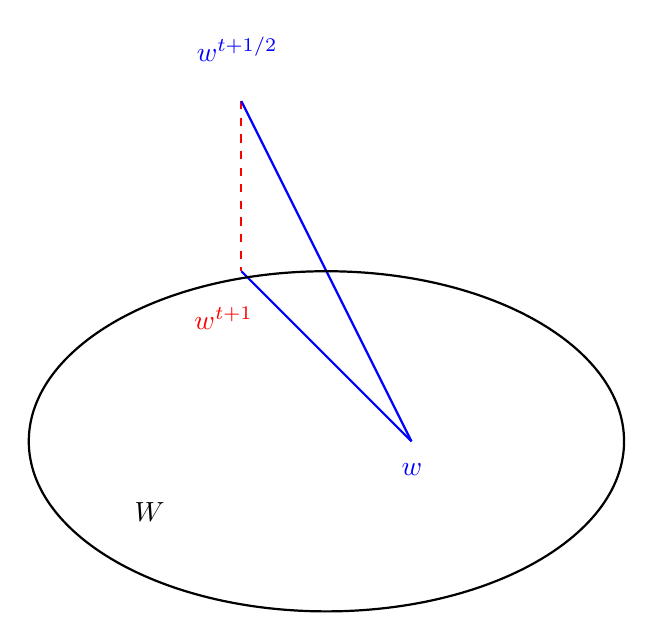
\begin{tikzpicture} [scale = 1] 
\node[red, right] at (3.6, 5.62){$w^{t+1}$};
\node[blue, right] at (3.63, 9.04){$w^{t+1/2}$};
\node[blue, right] at (6.23, 3.7){$w $};
\draw[red, dashed, thick] (4.32, 8.38) -- (4.32, 6.22);
\draw[blue, thick] (4.32, 8.38) -- (6.48, 4.06);
\draw[blue, thick] (4.32, 6.22) -- (6.48, 4.06);
\node[black, right] at (2.84, 3.16){$W $};
\draw[black, thick] (5.4, 4.06) ellipse (3.78 and 2.16);
\end{tikzpicture} 
\end{figure}
\begin{align*}
\displaystyle\sum_{t=1}^{T} \text{\;LHS\;} \boxed{1} &= \left\|w^{\left(T+1\right)} - w\right\|^{2} - \left\|w^{\left(1\right)} - w\right\|^{2}
\\ &\leq  \displaystyle\sum_{t=1}^{T} \text{\;RHS\;} \boxed{1} -= 2 \eta \displaystyle\sum_{t=1}^{T} \left(f_{t}\left(w^{t}\right) - f_{t}\left(w\right)\right) + \eta^{2} \displaystyle\sum_{t}^{T} \left\|\partial f_{t}\left(w^{t}\right)\right\|^{2}
\\ \displaystyle\sum_{t}^{T} f_{t}\left(w^{t}\right) - \displaystyle\sum_{t}^{T} f_{t}\left(w\right) &\leq  \dfrac{-\left\|w^{T+1} - w\right\|^{2} + \left\|w\right\|^{2}}{2 \eta} + \dfrac{\eta}{2} \displaystyle\sum_{t}^{T} \left\|\partial f_{t}\left(w^{t}\right)\right\|^{2}
\\ &\leq  \dfrac{\left\|w\right\|^{2}}{2 \eta} + \dfrac{\eta}{2} \displaystyle\sum_{t}^{T} \left\|\partial f_{t}\left(w^{t}\right)\right\|^{2} \leftarrow \boxed{2}
\end{align*}
Further assumptions:
\begin{enumerate}
\item $W $ is norm bounded: $\;\forall\; w \in W, \left\|w\right\| \leq  B $
\item $f_{t}, \;\forall\; t $ is $\rho$ Lipschitz $\left\|\partial f_{t}\left(w\right)\right\| \leq  \rho \;\forall\; w \in W $
\end{enumerate}

\begin{align*}
\boxed{2} &\stackrel{\text{\;Assump\;} 1.2}{\Rightarrow} \displaystyle\sum_{t}^{T} f_{t}\left(w^{t}\right) - \displaystyle\sum_{t}^{T} f_{t}\left(w\right) \leq  \dfrac{B^{2}}{2 \eta} + \dfrac{\eta}{2} \displaystyle\sum_{t}^{T} \rho^{2}
\\ &= \underbrace{\dfrac{B^{2}}{2 \eta} + \dfrac{\eta T \rho^{2}}{2} }_{\boxed{B \rho \sqrt{T}}}
\\ &  - \dfrac{B^{2}}{2 \eta^{2}} + \dfrac{T \rho^{2}}{2} = 0
\\ &  \eta = \sqrt{\dfrac{B^{2}}{T \rho^{2}}} = \dfrac{B}{\sqrt{T} \rho}
\end{align*}
doubling trick
\\* run OGD on $t  = 1$
\\* run OGD on $t  = 2, 3$
\\* run OGD on $t  = 4, 5, 6, 7$
\newline \newline




\section{Lecture $20$} 
passive learning: $\left(x , y\right) \sim  P_{XY}$ "unit cost" PAC w.p. $\geq  1 - \delta, n  = O\left(\dfrac{\left|  \mathcal{H}  \right|}{\varepsilon}\right)$
\\* active learning: $x  \sim  P_{X}$ free, query $x $, "oracle" gets $y  \sim  P_{Y | X = x}$, realizable $\left(y  = h^\star \left(x\right)\right)$ , unit cost, alg can choose $x  !$ adaptively
\\* e.x. $X  = 0: \dfrac{1}{N} : 1, \mathcal{H} = \left\{\mathbbm{1}_{\left(x \geq  a\right)}, a \in X\right\}, P_{X}$ unif $\left(X \right) \stackrel{iid}{\sim} n $ training items (passive)
\\* ERM, $h^{ERM} \in$ Version Space, $V  = \left\{h \in \mathcal{H} : h\left(x_{i}\right) = y_{i}, i = 1:n\right\}$
\begin{align*}
R\left(h^{ERM}\right)  &= O\left(\dfrac{1}{n}\right)
\end{align*}
\begin{figure}[H] \centering 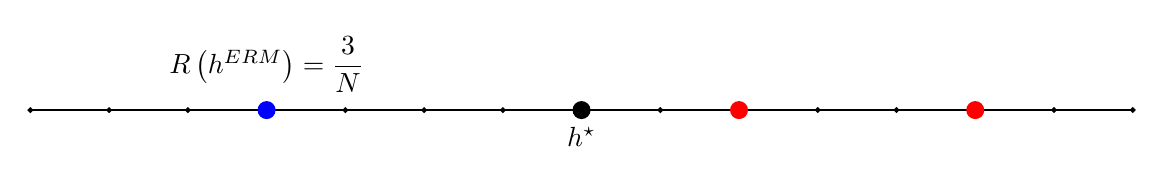
\begin{tikzpicture} [scale = 1] 
\draw[thick] (0.0, 0.0) -- (14.0, 0.0);
\draw[black, fill = black, thick] (0.0, 0.0) circle [radius = 0.02];
\draw[black, fill = black, thick] (1.0, 0.0) circle [radius = 0.02];
\draw[black, fill = black, thick] (2.0, 0.0) circle [radius = 0.02];
\draw[black, fill = black, thick] (3.0, 0.0) circle [radius = 0.02];
\draw[black, fill = black, thick] (4.0, 0.0) circle [radius = 0.02];
\draw[black, fill = black, thick] (5.0, 0.0) circle [radius = 0.02];
\draw[black, fill = black, thick] (6.0, 0.0) circle [radius = 0.02];
\draw[black, fill = black, thick] (7.0, 0.0) circle [radius = 0.02];
\draw[black, fill = black, thick] (8.0, 0.0) circle [radius = 0.02];
\draw[black, fill = black, thick] (9.0, 0.0) circle [radius = 0.02];
\draw[black, fill = black, thick] (10.0, 0.0) circle [radius = 0.02];
\draw[black, fill = black, thick] (11.0, 0.0) circle [radius = 0.02];
\draw[black, fill = black, thick] (12.0, 0.0) circle [radius = 0.02];
\draw[black, fill = black, thick] (13.0, 0.0) circle [radius = 0.02];
\draw[black, fill = black, thick] (14.0, 0.0) circle [radius = 0.02];
\draw[blue, fill = blue, thick] (3.0, 0.0) circle [radius = 0.1];
\draw[red, fill = red, thick] (12.0, 0.0) circle [radius = 0.1];
\draw[red, fill = red, thick] (9.0, 0.0) circle [radius = 0.1];
\draw[black, fill = black, thick] (7.0, 0.0) circle [radius = 0.1];
\node[below] at (7.0, -0.1){$h^\star $};
\node[above] at (3.0, 0.1){$R\left(h^{ERM}\right)  = \dfrac{3}{N}$};
\end{tikzpicture} 
\end{figure}
\begin{figure}[H] \centering 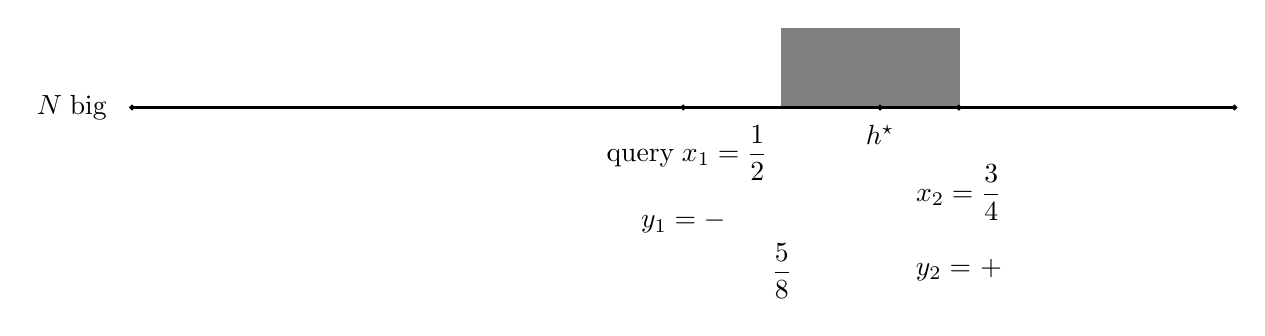
\begin{tikzpicture} [scale = 1] 
\draw[gray, fill = gray, thick] (8.25, 1.0) rectangle (10.5, 0.0);
\draw[thick] (0.0, 0.0) -- (14.0, 0.0);
\draw[black, fill = black, thick] (0.0, 0.0) circle [radius = 0.02];
\draw[black, fill = black, thick] (14.0, 0.0) circle [radius = 0.02];
\draw[black, fill = black, thick] (7.0, 0.0) circle [radius = 0.02];
\draw[black, fill = black, thick] (10.5, 0.0) circle [radius = 0.02];
\draw[black, fill = black, thick] (9.5, 0.0) circle [radius = 0.02];
\node[left] at (-0.1, 0.0){$N  \text{\;big\;}$};
\node[below] at (7.0, -0.1){$\text{\;query\;} x_{1} = \dfrac{1}{2}$};
\node[below] at (7.0, -1.2){$y_{1} = -$};
\node[below] at (10.5, -0.6){$x_{2} = \dfrac{3}{4}$};
\node[below] at (10.5, -1.8){$y_{2} =$ +};
\node[below] at (9.5, -0.1){$h^\star $};
\node[below] at (8.25, -1.6){$\dfrac{5}{8}$};
\end{tikzpicture} 
\end{figure}
$n $ queries
\begin{align*}
n  &= O\left(\log\left(\dfrac{1}{\varepsilon}\right)\right) \leq  R\left(h \in VS \right) = O\left(\dfrac{1}{2^{n}}\right)
\end{align*}
Unvertainty-based Active Learning
\begin{figure}[H] \centering 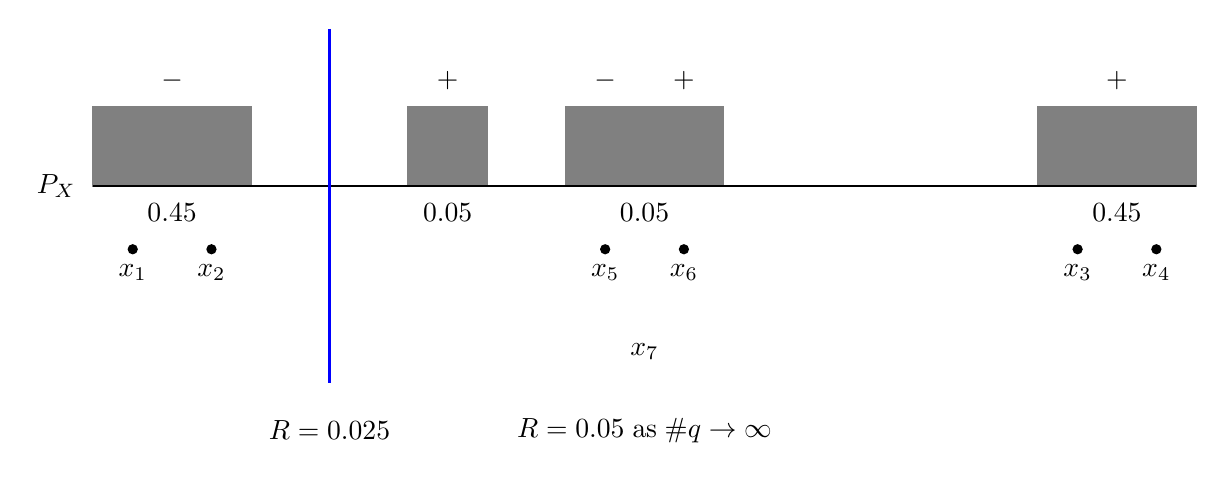
\begin{tikzpicture} [scale = 1] 
\draw[gray, fill = gray, thick] (0.0, 1.0) rectangle (2.0, 0.0);
\draw[gray, fill = gray, thick] (4.0, 1.0) rectangle (5.0, 0.0);
\draw[gray, fill = gray, thick] (6.0, 1.0) rectangle (8.0, 0.0);
\draw[gray, fill = gray, thick] (12.0, 1.0) rectangle (14.0, 0.0);
\draw[thick] (0.0, 0.0) -- (14.0, 0.0);
\node[above] at (1.0, 1.1){$-$};
\node[above] at (13.0, 1.1){$+$};
\node[above] at (6.5, 1.1){$-$};
\node[above] at (7.5, 1.1){$+$};
\node[above] at (4.5, 1.1){$+$};
\node[left] at (-0.1, 0.0){$P_{X}$};
\node[below] at (1.0, -0.1){$0.45$};
\node[below] at (13.0, -0.1){$0.45$};
\node[below] at (7.0, -0.1){$0.05$};
\node[below] at (4.5, -0.1){$0.05$};
\draw[black, fill = black, thick] (0.5, -0.8) circle [radius = 0.05];
\draw[black, fill = black, thick] (1.5, -0.8) circle [radius = 0.05];
\draw[black, fill = black, thick] (6.5, -0.8) circle [radius = 0.05];
\draw[black, fill = black, thick] (7.5, -0.8) circle [radius = 0.05];
\draw[black, fill = black, thick] (12.5, -0.8) circle [radius = 0.05];
\draw[black, fill = black, thick] (13.5, -0.8) circle [radius = 0.05];
\node[] at (0.5, -1.1){$x_{1}$};
\node[] at (1.5, -1.1){$x_{2}$};
\node[] at (6.5, -1.1){$x_{5}$};
\node[] at (7.5, -1.1){$x_{6}$};
\node[] at (7.0, -2.1){$x_{7}$};
\node[] at (12.5, -1.1){$x_{3}$};
\node[] at (13.5, -1.1){$x_{4}$};
\node[] at (7.0, -3.1){$R  = 0.05 \text{\;as\;} \# q \to  \infty$};
\draw[blue, thick] (3.0, 2.0) -- (3.0, -2.5);
\node[] at (3.0, -3.1){$R  = 0.025$};
\end{tikzpicture} 
\end{figure}
CAL
\\* init $V_{1} = \mathcal{H}$ version space
\\* for epoch $r  = 1, 2, ...$
\begin{align*}
x  &\sim  P_{X}
\end{align*}
if $V_{r}$ disagrees on $x  \left(\text{\;ie\;} \exists h, h' \in V_{r} , h\left(x\right) \neq  h'\left(x\right)\right)$
\\* query $x $ 's label, oracle gives $y $
\begin{align*}
V_{r+1} &= \left\{h \in V_{r} , h\left(x\right) = y \right\}
\end{align*}
init $V_{1} = \mathcal{H}$ version space
\\* for epoch $r  = 1, 2, ..., R $
\\* (make sure this happens $k $ times)
\begin{itemize}
\item $x  \sim  P_{X}$
\item if $V_{r}$ disagrees on $x  \left(\text{\;ie\;} \exists h, h' \in V_{r} , h\left(x\right) \neq  h'\left(x\right)\right)$
\item query $x $ 's label, oracle gives $y $
\end{itemize}\begin{align*}
V_{r+1} &= \left\{h \in V_{r} , h\left(x_{i}\right) = y_{i} , i = 1 ... k \right\}
\end{align*}
Output any $h  \in V_{R+1}$
\newline \newline
version space $V_{r}$
\\* Disagreement region $DIS  \left(V_{r}\right) := \left\{x \in X : \exists h, h' \in V_{r} : h\left(x\right) \neq  h'\left(x\right)\right\}$
\newline \newline
\begin{figure}[H] \centering 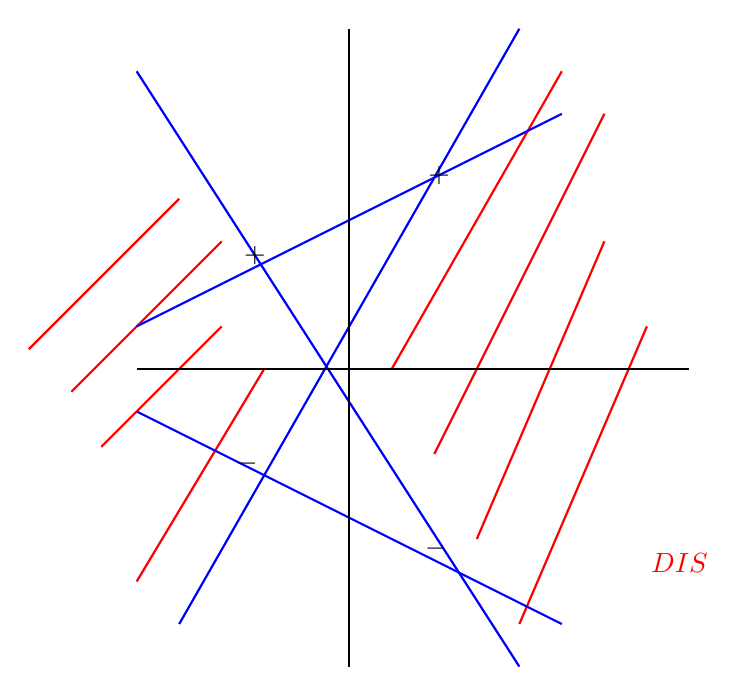
\begin{tikzpicture} [scale = 1] 
\node[red, right] at (8.03, 2.14){$DIS $};
\draw[red, thick] (3.24, 4.6) -- (1.62, 1.9);
\draw[red, thick] (2.7, 5.14) -- (1.17, 3.61);
\draw[red, thick] (2.7, 6.22) -- (0.79, 4.31);
\draw[red, thick] (2.16, 6.76) -- (0.25, 4.85);
\draw[red, thick] (8.1, 5.14) -- (6.48, 1.36);
\draw[red, thick] (7.56, 6.22) -- (5.94, 2.44);
\draw[red, thick] (7.56, 7.84) -- (5.4, 3.52);
\draw[red, thick] (7.02, 8.38) -- (4.86, 4.6);
\draw[blue, thick] (1.62, 4.06) -- (7.02, 1.36);
\draw[blue, thick] (1.62, 5.14) -- (7.02, 7.84);
\draw[blue, thick] (1.62, 8.38) -- (6.48, 0.82);
\draw[blue, thick] (6.48, 8.92) -- (2.16, 1.36);
\node[black, right] at (5.16, 2.32){$-$};
\node[black, right] at (2.76, 3.4){$-$};
\node[black, right] at (5.2, 7.06){$+$};
\node[black, right] at (2.86, 6.04){$+$};
\draw[black, thick] (4.32, 8.92) -- (4.32, 0.82);
\draw[black, thick] (1.62, 4.6) -- (8.64, 4.6);
\end{tikzpicture} 
\end{figure}
\begin{align*}
\Delta \left(V_{r}\right) :&= P_{X} \left(DIS  \left(V_{r}\right)\right)
\\ &R\left(h^{CAL}\right) 
\end{align*}
pseudometric $d\left(h, h'\right) , h, h' \in \mathcal{H} = \mathbb{E}_{x \sim  P_{X}} \mathbbm{1}_{\left(h\left(x\right) \neq  h'\left(x\right)\right)}$
\begin{align*}
&\Rightarrow  R\left(h\right) = d\left(h, h^\star \right)
\end{align*}
\begin{figure}[H] \centering 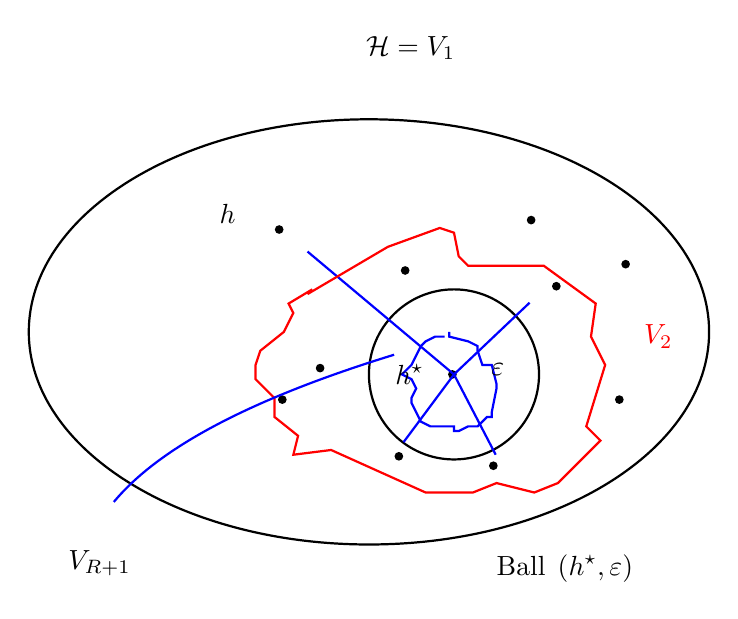
\begin{tikzpicture} [scale = 1] 
\draw[blue, thick] (5.82, 4.0) -- (5.7, 4.0) -- (5.58, 3.94) -- (5.52, 3.88) -- (5.4, 3.64) -- (5.28, 3.52) -- (5.28, 3.52) -- (5.4, 3.46) -- (5.46, 3.34) -- (5.4, 3.22) -- (5.4, 3.16) -- (5.52, 2.92) -- (5.64, 2.86) -- (5.7, 2.86) -- (5.76, 2.86) -- (5.88, 2.86) -- (5.94, 2.86) -- (5.94, 2.8) -- (6.0, 2.8) -- (6.12, 2.86) -- (6.24, 2.86) -- (6.36, 2.98) -- (6.42, 2.98) -- (6.42, 3.04) -- (6.48, 3.34) -- (6.48, 3.4) -- (6.42, 3.64) -- (6.36, 3.64) -- (6.3, 3.64) -- (6.24, 3.82) -- (6.24, 3.88) -- (6.12, 3.94) -- (5.88, 4.0) -- (5.88, 4.06);
\node[black, right] at (6.29, 3.58){$\varepsilon$};
\node[black, right] at (5.07, 3.52){$h^\star $};
\node[black, right] at (2.84, 5.56){$h $};
\node[black, right] at (6.26, 1.06){$\text{\;Ball\;} \left(h^\star , \varepsilon\right)$};
\draw[black, thick] (5.94, 3.52) ellipse (1.08 and 1.08);
\node[black, right] at (4.7, 7.66){$\mathcal{H} = V_{1}$};
\node[black, right] at (0.92, 1.12){$V_{R+1}$};
\draw[black, fill = black, thick] (5.92, 3.52) circle [radius = 0.04];
\draw[blue, thick] (5.94, 3.52) -- (4.08, 5.08);
\draw[blue, thick] (5.94, 3.52) -- (6.9, 4.43);
\draw[blue, thick] (5.94, 3.52) -- (6.47, 2.5);
\draw[blue, thick] (5.94, 3.52) -- (5.3, 2.66);
\draw[black, thick] (4.86, 4.06) ellipse (4.32 and 2.7);
\draw[black, fill = black, thick] (3.72, 5.36) circle [radius = 0.04];
\draw[black, fill = black, thick] (6.92, 5.48) circle [radius = 0.04];
\draw[black, fill = black, thick] (7.24, 4.64) circle [radius = 0.04];
\draw[black, fill = black, thick] (8.12, 4.92) circle [radius = 0.04];
\draw[black, fill = black, thick] (8.04, 3.2) circle [radius = 0.04];
\draw[black, fill = black, thick] (6.44, 2.36) circle [radius = 0.04];
\draw[black, fill = black, thick] (5.24, 2.48) circle [radius = 0.04];
\draw[black, fill = black, thick] (4.24, 3.6) circle [radius = 0.04];
\draw[black, fill = black, thick] (3.76, 3.2) circle [radius = 0.04];
\draw[black, fill = black, thick] (5.32, 4.84) circle [radius = 0.04];
\draw[red, thick] (4.08, 4.54) -- (5.1, 5.14) -- (5.76, 5.38) -- (5.94, 5.32) -- (6.0, 5.02) -- (6.12, 4.9) -- (7.08, 4.9) -- (7.74, 4.42) -- (7.68, 4.0) -- (7.86, 3.64) -- (7.62, 2.86) -- (7.8, 2.68) -- (7.26, 2.14) -- (6.96, 2.02) -- (6.48, 2.14) -- (6.18, 2.02) -- (5.58, 2.02) -- (4.38, 2.56) -- (3.9, 2.5) -- (3.96, 2.74) -- (3.66, 2.98) -- (3.66, 3.22) -- (3.42, 3.46) -- (3.42, 3.64) -- (3.48, 3.82) -- (3.78, 4.06) -- (3.9, 4.3) -- (3.84, 4.42) -- (4.14, 4.6);
\node[red, right] at (8.23, 4.0){$V_{2}$};
\draw[blue, thick] (1.62, 1.9).. controls(2.20, 2.60)and(3.39, 3.22)..(5.18, 3.77);
\end{tikzpicture} 
\end{figure}



\section{Lecture $21$} 

\subsection{CAL (mini-batch version)}
\begin{enumerate}
\item init $V_{1} = \mathcal{H}$ (assume $| \mathcal{H} | < \infty$)
\item FOR epoches $i  = 1 ... n $
\item Collect $k $ items $x_{1} , .. , x_{k} \stackrel{iid}{\sim} P_{X} \text{\;such that\;} \text{\;they\;} \in DIS  \left(V_{i}\right) = \left\{x \in X : \exists h, h' \in V_{i} , h\left(x\right) \neq  h'\left(x\right)\right\}$
\item query them. Oracle gives their labels $y_{1} ... y_{k}$
\item $V_{i+1} = \left\{h \in V_{i} : h\left(x_{i}\right) = y_{i} , \;\forall\; i \in \left[k\right]\right\}$
\item return any $h  \in V_{n+1}$
\end{enumerate}

Want: query complexity
\begin{align*}
&O\left(\log \dfrac{1}{\varepsilon}\right) 
\end{align*}
w.p. $\leq  1 - \delta$
\newline \newline
\begin{figure}[H] \centering 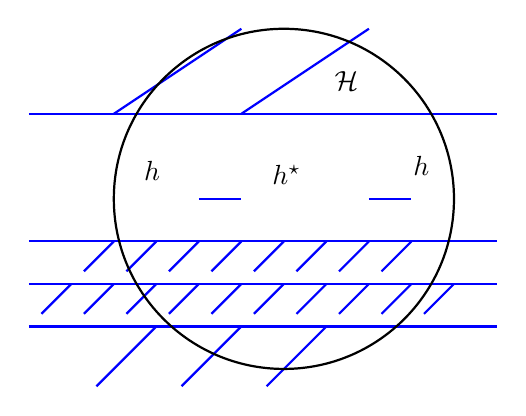
\begin{tikzpicture} [scale = 1] 
\node[black, right] at (5.38, 6.1){$\mathcal{H}$};
\draw[blue, thick] (4.32, 5.68) -- (5.94, 6.76);
\draw[blue, thick] (2.7, 5.68) -- (4.32, 6.76);
\draw[blue, thick] (5.94, 4.6) -- (6.48, 4.6);
\draw[blue, thick] (3.78, 4.6) -- (4.32, 4.6);
\draw[blue, thick] (6.48, 4.06) -- (6.1, 3.68);
\draw[blue, thick] (5.94, 4.06) -- (5.56, 3.68);
\draw[blue, thick] (5.4, 4.06) -- (5.02, 3.68);
\draw[blue, thick] (4.86, 4.06) -- (4.48, 3.68);
\draw[blue, thick] (4.32, 4.06) -- (3.94, 3.68);
\draw[blue, thick] (3.78, 4.06) -- (3.4, 3.68);
\draw[blue, thick] (3.24, 4.06) -- (2.86, 3.68);
\draw[blue, thick] (2.7, 4.06) -- (2.32, 3.68);
\draw[blue, thick] (7.02, 3.52) -- (6.64, 3.14);
\draw[blue, thick] (6.48, 3.52) -- (6.1, 3.14);
\draw[blue, thick] (5.94, 3.52) -- (5.56, 3.14);
\draw[blue, thick] (5.4, 3.52) -- (5.02, 3.14);
\draw[blue, thick] (4.86, 3.52) -- (4.48, 3.14);
\draw[blue, thick] (4.32, 3.52) -- (3.94, 3.14);
\draw[blue, thick] (3.78, 3.52) -- (3.4, 3.14);
\draw[blue, thick] (3.24, 3.52) -- (2.86, 3.14);
\draw[blue, thick] (2.7, 3.52) -- (2.32, 3.14);
\draw[blue, thick] (2.16, 3.52) -- (1.78, 3.14);
\draw[blue, thick] (5.4, 2.98) -- (4.64, 2.22);
\draw[blue, thick] (4.32, 2.98) -- (3.56, 2.22);
\draw[blue, thick] (3.24, 2.98) -- (2.48, 2.22);
\draw[blue, thick] (1.62, 2.98) -- (7.56, 2.98);
\draw[blue, thick] (1.62, 3.52) -- (7.56, 3.52);
\draw[blue, thick] (1.62, 4.06) -- (7.56, 4.06);
\draw[blue, thick] (1.62, 5.68) -- (7.56, 5.68);
\node[black, right] at (6.38, 5.02){$h $};
\node[black, right] at (2.96, 4.96){$h $};
\node[black, right] at (4.59, 4.9){$h^\star $};
\draw[black, thick] (4.86, 4.6) ellipse (2.16 and 2.16);
\end{tikzpicture} 
\end{figure}
\begin{align*}
P_{X}\left(DIS  \left(V_{i}\right)\right) &\geq  R\left(h\right), \;\forall\; h \in V_{i}
\end{align*}
Define (pseudo) metric
\begin{align*}
&  d\left(h, h'\right)  = P_{x}\left(DIS\left(\left\{h, h'\right\}\right) \right)
\\ &\Rightarrow  d\left(h, h^\star \right) = \mathbb{E}_{x \sim  P_{X}} \mathbbm{1}_{\left(h\left(x\right) \neq  h^\star \left(x\right)\right)} = R\left(h\right) 
\end{align*}
Want:
\begin{align*}
&  \boxed{P_{X}\left(DIS\left(V_{i+1}\right) \right) \leq  \dfrac{1}{2} P_{x}\left(DIS\left(V_{i}\right) \right) \;\forall\; i \in \left[n\right]}
\\ &\Rightarrow  R\left(h\right) \in V_{n+1} \leq  P_{X}\left(DIS\left(V_{n+1}\right) \right) \leq  \dfrac{1}{2^{n}} := \varepsilon \Rightarrow  R\left(h\right) < \varepsilon \text{\;if\;} n = \log\left(\dfrac{1}{\varepsilon}\right)
\end{align*}
\begin{figure}[H] \centering 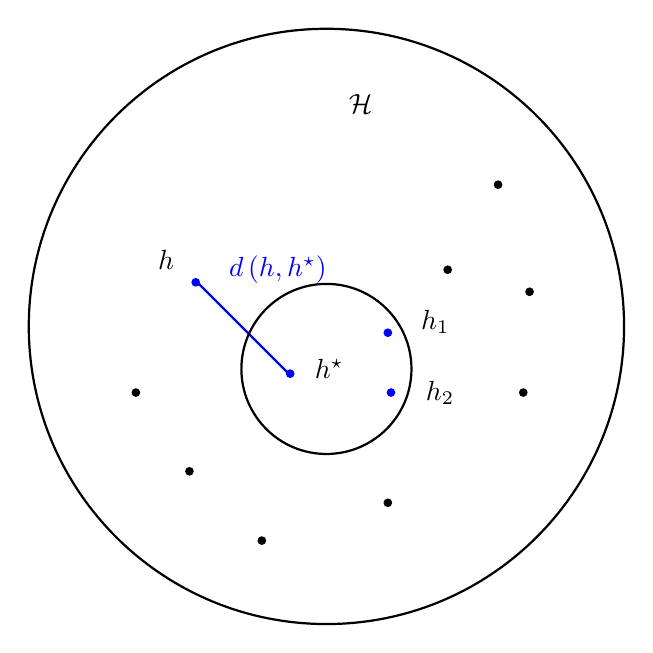
\begin{tikzpicture} [scale = 1] 
\node[black, right] at (5.02, 7.42){$\mathcal{H}$};
\draw[black, fill = black, thick] (2.44, 3.76) circle [radius = 0.04];
\draw[black, fill = black, thick] (7.04, 6.4) circle [radius = 0.04];
\draw[black, fill = black, thick] (6.4, 5.32) circle [radius = 0.04];
\draw[black, fill = black, thick] (7.44, 5.04) circle [radius = 0.04];
\draw[black, fill = black, thick] (7.36, 3.76) circle [radius = 0.04];
\draw[black, fill = black, thick] (5.64, 2.36) circle [radius = 0.04];
\draw[black, fill = black, thick] (4.04, 1.88) circle [radius = 0.04];
\draw[black, fill = black, thick] (3.12, 2.76) circle [radius = 0.04];
\draw[blue, fill = blue, thick] (5.68, 3.76) circle [radius = 0.04];
\draw[blue, fill = blue, thick] (5.64, 4.52) circle [radius = 0.04];
\draw[blue, fill = blue, thick] (4.4, 4.0) circle [radius = 0.04];
\draw[blue, fill = blue, thick] (3.2, 5.16) circle [radius = 0.04];
\draw[blue, thick] (3.24, 5.14) -- (4.39, 3.99);
\node[blue, right] at (3.5, 5.32){$d\left(h, h^\star \right) $};
\node[black, right] at (6.0, 3.76){$h_{2}$};
\node[black, right] at (5.94, 4.66){$h_{1}$};
\node[black, right] at (4.59, 4.06){$h^\star $};
\node[black, right] at (2.6, 5.44){$h $};
\draw[black, thick] (4.86, 4.06) ellipse (1.08 and 1.08);
\draw[black, thick] (4.86, 4.6) ellipse (3.78 and 3.78);
\end{tikzpicture} 
\end{figure}
\begin{align*}
B\left(h^\star , r\right)  :&= \left\{h \in \mathcal{H}, d\left(h, h^\star \right) \leq  r\right\}
\\ &P_{X}\left(DIS\left(B\left(h^\star , r\right)\right) \right)
\end{align*}
\begin{figure}[H] \centering \begin{tikzpicture} [scale = 1] 
\draw[red, thick] (3.78, 5.68) ellipse (3.24 and 3.24);
\draw[red, thick] (3.24, 6.22) ellipse (1.62 and 1.62);
\draw[red, thick] (3.24, 6.22) ellipse (0.54 and 0.54);
\draw[blue, thick] (5.94, 7.3) -- (6.73, 7.97);
\draw[blue, thick] (5.94, 7.3) -- (6.24, 8.4);
\draw[blue, thick] (5.4, 5.14) -- (5.37, 2.56);
\draw[blue, thick] (5.4, 5.14) -- (4.32, 2.72);
\draw[blue, thick] (5.94, 7.3) -- (6.48, 7.3);
\draw[blue, thick] (5.94, 7.84) -- (6.48, 7.84);
\draw[blue, thick] (3.78, 2.98) -- (5.4, 2.98);
\draw[blue, thick] (4.32, 3.52) -- (5.4, 3.52) -- (5.94, 3.52);
\draw[blue, thick] (4.32, 4.06) -- (5.94, 4.06);
\draw[blue, thick] (4.86, 4.6) -- (5.94, 4.6);
\node[black, right] at (7.02, 3.94){$-$};
\node[black, right] at (7.44, 5.44){$-$};
\node[black, right] at (3.25, 5.02){+};
\node[black, right] at (4.09, 7.0){+};
\node[black, right] at (5.88, 1.9){$h_{2}$};
\node[black, right] at (3.96, 2.02){$h_{1}$};
\node[black, right] at (7.23, 8.26){$h^\star $};
\draw[black, thick] (6.48, 8.38) -- (4.86, 1.9);
\draw[black, thick] (5.94, 8.38) -- (5.94, 2.44);
\draw[black, thick] (7.02, 7.84) -- (3.24, 2.98);
\end{tikzpicture} 
\end{figure}
\begin{align*}
V_{i} &= \left\{h^\star , h_{1}, h_{2}\right\}
\end{align*}
Step $3 =$ draw iid $P_{X | V_{i}}$
\begin{align*}
&\boxed{P_{X | V_{i}} = \dfrac{P\left(x\right)}{\displaystyle\int_{x' \in DIS\left(V_{i}\right) } P\left(x'\right) d x'} = \dfrac{P\left(x\right)}{P_{X}\left(DIS\left(V_{i}\right) \right)}}
\end{align*}
Define $Q_{X Y} := P_{X | V_{i}} \cdot  P\left(Y | X\right)$
\begin{align*}
R_{Q}\left(h\right) &= \dfrac{R_{P}\left(h\right)}{P_{X}\left(DIS\left(V_{i}\right) \right)}
\end{align*}
Want:
\begin{align*}
P_{X}\left(DIS\left(V_{i+1}\right) \right) &\leq  f\left(r_{V_{i+1}}\right), r_{V} := \displaystyle\max_{h \in V} d\left(h, h^\star \right)
\end{align*}
\begin{figure}[H] \centering \begin{tikzpicture} [scale = 1] 
\draw[blue, fill = blue, thick] (7.36, 4.24) circle [radius = 0.04];
\draw[blue, fill = blue, thick] (4.64, 5.88) circle [radius = 0.04];
\node[black, right] at (7.06, 5.92){$V_{i}$};
\node[black, right] at (4.41, 5.56){$h^\star $};
\node[blue, right] at (5.33, 5.08){$r $};
\draw[red, thick] (4.86, 5.14) -- (8.1, 2.44);
\draw[blue, thick] (4.86, 5.14) -- (5.62, 4.38);
\draw[blue, fill = blue, thick] (4.84, 5.16) circle [radius = 0.04];
\draw[blue, thick] (4.86, 5.14) ellipse (1.08 and 1.08);
\draw[red, thick] (4.86, 4.6) ellipse (3.78 and 3.78);
\draw[black, thick] (4.86, 6.76).. controls(4.05, 6.94)and(3.26, 7.29)..(2.71, 6.49).. controls(2.29, 5.89)and(2.01, 5.56)..(2.23, 4.93).. controls(2.6, 3.9)and(4.31, 5.07)..(4.86, 4.6).. controls(5.31, 4.21)and(4.96, 3.71)..(5.32, 2.46).. controls(5.67, 1.23)and(6.7, 1.75)..(7.42, 1.97).. controls(8.85, 2.41)and(9.01, 5.75)..(8.1, 6.22).. controls(7.41, 6.58)and(6.1, 6.48)..(4.86, 6.76);
\end{tikzpicture} 
\end{figure}
\begin{align*}
d\left(h, h^\star \right)  &= R_{P}\left(h\right) = R_{X}\left(DIS\left(V_{i}\right) \right) \cdot  R_{Q}\left(h\right), \;\forall\; h \in V_{i}
\end{align*}
Suppose $h  \in V_{i}$ survives $k $ iid $Q $
\begin{align*}
&\Rightarrow  R_{Q}\left(h\right) \text{\;small\;} := r
\\ &  \left|  V_{i}  \right| \cdot  \left[\left(1 - r\right)^{k}\right] \leq  \left|  V_{i}  \right| e^{-r k} := \dfrac{\delta}{n}
\\ &  -r k = \log \dfrac{\delta}{n \left|  V_{i}  \right|}
\\ &\Rightarrow  k = \dfrac{\log \dfrac{n \left|  V_{i}  \right|}{\delta}}{r}
\end{align*}
\begin{figure}[H] \centering \begin{tikzpicture} [scale = 1] 
\node[blue, right] at (6.39, 1.96){$1 - r $};
\node[blue, right] at (6.19, 5.68){$e^{-r}$};
\draw[blue, thick] (2.7, 7.3).. controls(4.12, 5.79)and(5.59, 4.96)..(7.11, 4.79);
\draw[blue, thick] (2.7, 6.76) -- (7.02, 2.44);
\draw[black, thick] (4.32, 7.84) -- (4.32, 1.9);
\draw[black, thick] (2.16, 4.06) -- (7.02, 4.06);
\end{tikzpicture} 
\end{figure}




\section{Lecture $22$} 

\subsection{Missed Lecture}
\begin{align*}
&V_{i}
\\ Q  :&= P_{X | DIS\left(V_{i}\right) } \cdot  P_{Y | X}
\\ R_{Q}\left(h\right) :&= \dfrac{R_{p}\left(h\right)}{P_{X}\left(DIS\left(V_{i}\right) \right)}
\end{align*}
$k $ labeled items $\stackrel{iid}{\sim} Q $
\begin{align*}
wp  &\geq  1 - \dfrac{\delta}{n}, \underbrace{\;\forall\; h \in V_{i+1}}_{\text{\;agrees on those\;} k \text{\;items\;}}, R_{Q}\left(h\right) \leq  r \text{\;if\;} k \geq  \dfrac{\log \dfrac{n \left|  V_{i}  \right|}{\delta}}{r}
\\ &\Rightarrow  \underbrace{R_{p}\left(h\right)}_{= d\left(h, h^\star \right)} \leq  P_{X}\left(DIS\left(V_{i}\right) \right) \cdot  r
\\ &\Rightarrow  V_{i+1} \subseteq B\left(h^\star , P_{X}\left(DIS\left(V_{i}\right) \right) \cdot  r\right)
\\ d\left(h, h^\star \right)  &= \mathbb{E}_{x \sim  P_{X}} \mathbbm{1}_{\left(h\left(x\right) \neq  h^\star \left(x\right)\right)}
\\ &= P_{X}\left(DIS\left(\left\{h, h^\star \right\}\right) \right)
\end{align*}
want:
\begin{align*}
&  P_{X}\left(DIS\left(V_{i+1}\right) \right) \leq  \dfrac{1}{2} P_{X}\left(DIS\left(V_{i}\right) \right)
\\ &\Rightarrow  \underbrace{P_{X}\left(DIS\left(V_{n+1}\right) \right)}_{d\left(h, h^\star \right) \;\forall\; h \in V_{n+1}} \leq  \dfrac{1}{2^{n}} P_{X}\left(DIS\left(V_{1} = \mathcal{H}\right) \right) \leq  \dfrac{1}{2^{n}} = \varepsilon
\end{align*}
set $n  = \log \dfrac{1}{\varepsilon}$
\begin{align*}
&  P_{X}\left(DIS\left(\overbrace{B\left(h^\star , \tau\right)}^{\left\{h \in \mathcal{H} : d\left(h, h^\star \right) \leq  \tau\right\}}\right) \right)
\\ &  \theta := \displaystyle\sup_{\tau \in \left(0, 1\right)} \dfrac{P_{X}\left(DIS\left(B\left(h^\star , \tau\right)\right) \right)}{\tau} \left(\text{\;Assume\;} \theta < \infty\right) \leftarrow \left(\text{\;disagreement coefficient\;}\right)
\\ &\Rightarrow  \;\forall\; \tau \in \left(0, 1\right), P_{X}\left(DIS\left(B\left(h^\star , \tau\right)\right) \right) \leq  \theta \tau
\\ &  P_{X}\left(DIS\left(V_{i+1}\right) \right) \leq  P_{X}\left(DIS\left(B\left(h^\star , P_{X}\left(DIS\left(V_{i}\right) \right) r\right)\right) \right) \leq  \theta P_{X}\left(DIS\left(V_{i}\right) \right) r 
\end{align*}
\begin{figure}[H] \centering \begin{tikzpicture} [scale = 1] 
\draw[blue, thick] (2.16, 3.52).. controls(8.58, 3.88)and(3.58, 5.23)..(7.02, 5.68);
\draw[blue, thick] (2.16, 3.52).. controls(4.05, 5.19)and(5.63, 6.06)..(6.91, 6.14);
\draw[blue, thick] (2.16, 3.52).. controls(3.04, 5.37)and(4.52, 6.32)..(6.63, 6.39);
\node[black, right] at (1.71, 6.22){$1$};
\node[black, right] at (2.01, 2.98){$0$};
\node[black, right] at (7.39, 3.1){$\tau$};
\draw[black, ->, thick] (2.16, 3.52) -- (2.16, 6.22);
\draw[black, ->, thick] (2.16, 3.52) -- (7.56, 3.52);
\end{tikzpicture} 
\end{figure}
Choose $r  = \dfrac{1}{2 \theta}, k \geq  \dfrac{\log \dfrac{n \left|  V_{i}  \right|}{\delta}}{\dfrac{1}{2 \theta}}$
\\* Set $k  = \dfrac{\log \dfrac{n \left|  V_{i}  \right|}{\delta}}{\dfrac{1}{2 \theta}} = 2 \theta \left[\log \log \dfrac{1}{\varepsilon} + \log \dfrac{\left|  \mathcal{H}  \right|}{\delta}\right]$
\\* Total number queries by CAL
\begin{align*}
k  \cdot  n &= 2 \theta \left[\log \log \dfrac{1}{\varepsilon} + \log \dfrac{\left|  \mathcal{H}  \right|}{\delta}\right] \log \dfrac{1}{\varepsilon}
\end{align*}


\subsection{End Missed Lecture}


\subsection{Stochastic Bandits}
Arms $1 ... K $
\\* Unknown but fixed reward distributions $V_{1} ... V_{k}$ with means $U_{1} ... U_{k} \in \mathbb{R}$
\\* $n $ total rounds
\\* (pseudo) regret
\begin{align*}
U^\star  &= \displaystyle\max_{i \in \left[k\right]} U_{i}
\end{align*}
Let $I_{t} \in \left[k\right]$ be the arm you pull at round $t , t \in \left[n\right]$
\\* Let $X_{t}$ be the reward you see at round $t $
\begin{align*}
&n  U^\star  - \displaystyle\sum_{t=1}^{n} \mathbb{E} U_{I_{t}}
\end{align*}
exploration then exploitation
\begin{enumerate}
\item pull each arm $m $ times, estimate $\hat{U}_{i}, i \in \left[k\right]$
\item for $n  - m  k $ rounds, pull $I_{t} := \arg\displaystyle\max \hat{U}_{i}$
\end{enumerate}





\section{Lecture $23$} 

\subsection{Subgraussian tail bounds}
Let $X_{i = 1 ... n} - u $ be independent $\sigma$ subgaussian random variables. Then,
\begin{align*}
&  \mathbb{P}\left(\hat{u} \geq  u + \varepsilon\right) \leq  e^{- \dfrac{n \varepsilon^{2}}{2 \sigma^{2}}}
\\ &  \text{\;wp\;} \geq  1 - \delta, u \leq  \hat{u} + \sqrt{\dfrac{2 \sigma^{2} \log \dfrac{1}{\delta}}{n}}
\end{align*}


\subsection{K-arm bandit (stochastic)}
"environment" $k $ arms with reward
\\* distributions $V_{1} ... V_{k}, 1$-subgaussian
\\* with mean $U_{1} ... U_{k}$
\\* def: $U^\star  = \displaystyle\max_{i \in \left[k\right]} U_{i}$
\\* (assume $U_{1} \geq  U_{2} \geq  ... \geq  U_{k}$)
\\* def: $\Delta_{i} = U_{1} - U_{i}, i \in \left[k\right]$
\newline \newline
"learner, agent"
\\* knows: $k  , 1$-subgaussian, $n $ time horizon, $I_{t} =$ "policy" $\text{\;alg\;} \left(I_{1}, X_{1}, .. I_{t-1}, X_{t-1}\right) , X_{t} \sim  V_{I_{t}}, T_{i}\left(t\right)$, number of arm $i $ pulls up to time $t $
\\* Goal: minimize (psuedo) regret
\begin{align*}
Reg  :&= n U^\star  - \displaystyle\sum_{t=1}^{n} \mathbb{E} U_{I_{t}}
\end{align*}
Alg: exploration-then-exploitation $\left(m \right)$
\begin{enumerate}
\item pull each arm $m $ times $\Rightarrow  \hat{U}_{t} , i \in \left[k\right]$
\item For remaining $n  - m k $ pulls, $\arg\displaystyle\max_{i \in \left[k\right]} \hat{U}_{i}$
\end{enumerate}

\begin{align*}
m  \Delta_{1} + m \Delta_{2} + ... + m \Delta_{k} &= m \displaystyle\sum_{i=1}^{k} \Delta_{i} = \dfrac{n}{k} \displaystyle\sum \Delta_{i}
\end{align*}
\begin{align*}
Reg  &= \displaystyle\sum_{i=1}^{k} \mathbb{E}\left(T_{i}\left(n\right)\right) \Delta_{i}
\\ \mathbb{E} T_{i}\left(n\right) &= m + \left(n - m k\right) \mathbb{P}\left(I = i\right)
\\ &= m + \left(n - m k\right) \mathbb{P}\left(\hat{U}_{i} \geq  \displaystyle\max_{j \in \left[k\right], j \neq  i} \hat{U}_{j}\right)
\\ &\leq  m + \left(n - m k\right) \mathbb{P}\left(\hat{U}_{i} \geq  \hat{U}_{1}\right)
\\ &= m + \left(n - m k\right) + \mathbb{P}\left(\hat{U}_{i} \leq  \hat{U}_{1} + U_{i} - U_{i} + \Delta_{i}\right)
\\ &= m + \left(n - m k\right) + \mathbb{P}\left(\left(\hat{U}_{i} - U_{i}\right)  - \left(\hat{U}_{1} - U_{1}\right) \geq  \Delta_{i}\right)
\\ &\leq  m + \left(n - m k\right) e^{- \dfrac{\Delta_{i}}{2 \left(\dfrac{2}{m}\right)}}
\end{align*}
\begin{figure}[H] \centering \begin{tikzpicture} [scale = 1] 
\node[black, right] at (4.64, 4.66){$\Rightarrow $};
\node[blue, right] at (6.62, 4.6){$\Delta_{i}$};
\draw[blue, <->, thick] (6.48, 5.14) -- (6.48, 4.06);
\draw[blue, ->, thick] (7.56, 3.52) -- (7.56, 4.6);
\draw[blue, ->, thick] (5.4, 5.68) -- (5.4, 4.6);
\draw[black, thick] (6.48, 2.98) -- (7.02, 2.98);
\draw[black, thick] (3.78, 2.98) -- (4.32, 2.98);
\draw[black, thick] (2.16, 2.44) -- (3.24, 2.44);
\draw[black, thick] (2.16, 2.98) -- (3.24, 2.98);
\draw[black, thick] (1.62, 3.52) -- (3.24, 3.52);
\draw[black, thick] (3.24, 4.06) -- (4.32, 4.06);
\draw[black, thick] (7.02, 6.22) -- (8.1, 6.22);
\draw[black, thick] (5.94, 3.52) -- (8.1, 3.52);
\draw[black, thick] (5.4, 4.06) -- (7.02, 4.06);
\draw[black, thick] (5.94, 5.14) -- (8.1, 5.14);
\draw[black, thick] (5.4, 5.68) -- (7.56, 5.68);
\draw[black, thick] (1.62, 5.68) -- (3.24, 5.68);
\node[black, right] at (0.88, 6.28){$\hat{U}_{i}$};
\node[black, right] at (7.97, 3.34){$\hat{U}_{1}$};
\node[black, right] at (8.31, 5.14){$U_{1}$};
\node[black, right] at (5.06, 3.94){$U_{i}$};
\node[black, right] at (5.02, 6.28){$\hat{U}_{i}$};
\draw[black, thick] (4.86, 7.3) -- (4.86, 1.9);
\end{tikzpicture} 
\end{figure}
\begin{align*}
\hat{U}_{i} &= \dfrac{1}{m} \displaystyle\sum_{t = 1, I_{t} = i}^{m k} X_{t}, X_{t} \stackrel{iid}{\sim} V_{i}, X_{t} - U_{i}, 1-\text{subgaussian}
\\ &\Rightarrow  \hat{U}_{i} - U_{i}, \dfrac{1}{\sqrt{m}}-\text{subgaussian} \;\forall\; i 
\\ &\Rightarrow  \left(\hat{U}_{i} - U_{i}\right) - \left(\hat{U}_{1} - U_{1}\right), \sqrt{\dfrac{2}{m}}-\text{subgaussian}
\end{align*}
\begin{align*}
\mathbb{P}\left(X \geq  \Delta_{i}\right) &\leq  e^{- \dfrac{\Delta_{i}^{2}}{2 \sigma^{2}}}
\end{align*}
\begin{figure}[H] \centering \begin{tikzpicture} [scale = 1] 
\node[black, right] at (5.27, 6.58){$N\left(0, \sigma^{2}\right) $};
\draw[black, thick] (1.62, 3.52)to [out = 0, in = 180](4.87, 6.61)to [out = 0, in = 180](7.88, 3.39);
\node[black, right] at (6.02, 2.26){$\Delta_{i}$};
\node[black, right] at (4.77, 1.9){$0$};
\draw[black, thick] (4.86, 7.3) -- (4.86, 2.44);
\draw[black, thick] (1.62, 2.98) -- (8.1, 2.98);
\end{tikzpicture} 
\end{figure}
\begin{align*}
Reg  &= \displaystyle\sum_{i=1}^{k} \mathbb{E} T_{i}\left(n\right)
\\ &\leq  \displaystyle\sum_{i=1}^{k} \left(m + \left(n - m k\right) e^{- \dfrac{\Delta_{i}^{2} m}{4}}\right) \Delta_{i}
\\ &\leq  \displaystyle\sum_{i}^{k} \left(m + n e^{- \dfrac{\Delta_{i}^{2} m}{4}}\right) \Delta_{i}
\\ &\leq  \displaystyle\sum_{i}^{k} \left(m + n e^{- \dfrac{\Delta_{2}^{2} m}{4}}\right) \Delta_{2}
\end{align*}
\begin{align*}
&  \dfrac{\partial \text{\;RHS\;}\left(m \right)}{\partial m} = 0
\\ &\Rightarrow  \displaystyle\sum_{i=1}^{k} \Delta_{i} \left(1 - k e^{- \dfrac{\Delta_{i}^{2} m}{4}} + \left(n - m k\right) e^{- \dfrac{\Delta_{i}^{2} m}{4}} \left(- \dfrac{\Delta_{i}^{2}}{4}\right)\right)
\\ &= \displaystyle\sum_{i} \Delta_{i} \left(1 - \left[k + \left(n - m k\right) \dfrac{\Delta_{i}^{2}}{4} \right] e^{- \dfrac{\Delta_{i}^{2} m}{4}}\right)
\\ &\approx  \displaystyle\sum_{i} \Delta_{i} \left(1 - \left[k + n \dfrac{\Delta_{i}^{2}}{4} \right] e^{- \dfrac{\Delta_{i}^{2} m}{4}}\right)
\\ &  ...
\end{align*}
\begin{align*}
&  \dfrac{\partial \text{\;RHS\;}\left(m \right)}{\partial m} = 0
\\ &\Rightarrow  \displaystyle\sum_{i} \Delta_{i} \left(1 - \dfrac{n \Delta_{2}^{2}}{4} e^{- \dfrac{\Delta_{2}^{2} m}{4}}\right) = 0
\\ &\Rightarrow  \displaystyle\sum \Delta_{i} = \left(\displaystyle\sum \dfrac{n \Delta_{2}^{2} \Delta_{i}}{4}\right) e^{- \dfrac{\Delta_{2}^{2} m}{4}}
\\ &\Rightarrow  \dfrac{4}{\Delta_{2}^{2}} \log \dfrac{\displaystyle\sum \dfrac{n \Delta_{2}^{2} \Delta_{i}}{4}}{\displaystyle\sum \Delta_{i}} = m = \dfrac{4}{\Delta_{2}^{2}} \log \dfrac{n \Delta_{2}^{2}}{4}
\end{align*}




\section{Lecture $24$} 
\begin{align*}
U_{1} &\geq  ... \geq  U_{k}
\\ \Delta_{i} &= U_{1} - U_{i} , i \in \left[k\right]
\\ Reg  :&= n U_{1} - \displaystyle\sum_{t=1}^{n} \mathbb{E}\left[U_{I_{t}}\right]
\\ &= \displaystyle\sum_{i=1}^{k} \Delta_{i} \mathbb{E}\left[T_{i}\left(n\right)\right]
\\ &\leq  \left(m + n e^{- \dfrac{\Delta_{2}^{2} m}{4}}\right) \left(\displaystyle\sum \Delta_{i}\right) \leftarrow \boxed{1}
\\ \text{\;optimal\;} m &= \dfrac{4}{\Delta_{2}^{2}} \log \dfrac{n \Delta_{2}^{2}}{4}
\\ \boxed{1} &\stackrel{m}{=} \left(\dfrac{4}{\Delta_{2}^{2}} \log \dfrac{n \Delta_{2}^{2}}{4} + n \left[e^{m}\right]^{- \dfrac{\Delta_{2}^{2}}{4}}\right) \displaystyle\sum \Delta_{i}
\\ &= \left(\dfrac{4}{\Delta_{2}^{2}} \log \dfrac{n \Delta_{2}^{2}}{4} + n \left[\dfrac{n \Delta_{2}^{2}}{4}\right]^{\dfrac{4}{\Delta_{2}^{2}} \left(- \dfrac{\Delta_{2}^{2}}{4}\right)}\right) \displaystyle\sum \Delta_{i}
\\ &= \left(\dfrac{4}{\Delta_{2}^{2}} \log \dfrac{n \Delta_{2}^{2}}{4} + \dfrac{4}{\Delta_{2}^{2}}\right) \displaystyle\sum \Delta_{i}
\\ &= \dfrac{4}{\Delta_{2}^{2}} \left(1 + \log \dfrac{n \Delta_{2}^{2}}{4}\right) \left(\displaystyle\sum \Delta_{i}\right)
\\ &\stackrel{k = 2, \Delta := \Delta_{2}}{=} \dfrac{4}{\Delta} \dfrac{1 + \log \left(n \Delta^{2}\right)}{4} \leftarrow \boxed{2}
\end{align*}
Alg needs $\Delta, k, n $
\\* Worst case $\Delta$
\newline \newline
\begin{align*}
\dfrac{\partial \boxed{2}}{\partial \Delta} &= 0
\\ - \dfrac{4}{\Delta^{2}} \left(1 + \log \dfrac{n \Delta^{2}}{4}\right) + \dfrac{4}{\Delta} \dfrac{4}{n \Delta^{2}} \dfrac{2 n \Delta}{4} &= 0
\\ - \dfrac{4}{\Delta^{2}} - \dfrac{4}{\Delta^{2}} \log \dfrac{n \Delta^{2}}{4} + \dfrac{8}{\Delta^{2}} &= 0
\\ \dfrac{4}{\Delta^{2}} &= \dfrac{4}{\Delta^{2}} \log \dfrac{n \Delta^{2}}{4}
\\ \dfrac{n \Delta^{2}}{4} &= e 
\\ \Delta^\star  &= \sqrt{\dfrac{4 e}{n}}
\\ \boxed{2} &\stackrel{\Delta^\star }{=} \dfrac{4 \sqrt{n}}{\sqrt{4 e}} \left(1 + \log \dfrac{n \dfrac{4 e}{n}}{4}\right)
\\ &= \dfrac{8 \sqrt{n}}{\sqrt{4 e}} = \dfrac{4}{\sqrt{e}} \sqrt{n}
\end{align*}

\subsection{Upper Confidence Bound (UCB)}
\begin{align*}
x_{1} ... x_{t} &\sim  V \left(1-\text{subgaussian}\right)
\\ U :&= \dfrac{1}{t} \displaystyle\sum_{\tau=1}^{t} x_{\tau} \leq  \hat{U}_{t} + \sqrt{\dfrac{2 \log \dfrac{1}{\delta}}{t}} \text{\;wp\;} 1 - \delta
\end{align*}
\begin{figure}[H] \centering \begin{tikzpicture} [scale = 1] 
\draw[blue, thick] (7.02, 6.76).. controls(7.25, 6.64)and(7.28, 5.91)..(7.12, 4.57);
\node[blue, right] at (7.57, 5.74){$U$};
\node[black, right] at (5.37, 4.78){$\hat{U}_{t}$};
\draw[black, thick] (4.32, 3.52).. controls(4.67, 2.8)and(4.97, 2.76)..(5.22, 3.4);
\draw[black, thick] (4.32, 6.22).. controls(4.69, 6.83)and(4.97, 6.91)..(5.15, 6.46);
\draw[black, thick] (4.86, 4.6) -- (5.4, 4.6);
\draw[black, thick] (4.32, 4.6) -- (4.86, 4.6);
\draw[black, thick] (4.86, 6.76) -- (4.86, 2.98);
\end{tikzpicture} 
\end{figure}
UCB(arm $i $, count $t $ of arm $i $ pulls) :$=$
\[ \left\{ \begin{array}{ll}
\hat{U}_{i t} + \sqrt{\dfrac{2 \log \dfrac{1}{\delta}}{t}}& \text{\;if\;} t > 0 \\
\infty& \text{\;if\;} t = 0 \\
\end{array}\right. \]
Alg:
\\* for $j  = 1 ... n $
\\* pull $I_{j} \in \arg\displaystyle\max_{i \in \left[t\right]} UCB\left(i, t_{i}\right) $
\newline \newline
\begin{align*}
Reg  :&= \displaystyle\sum_{i=1}^{k} \Delta_{i} \mathbb{E} T_{i}\left(n\right)
\end{align*}
idea:
\begin{align*}
\left[\;\forall\; t : UCB\left(1, t\right)  > U_{1}\right] :&= \text{\;Event\;} 1
\end{align*}
Fix $i  \neq  1$, fix a magic number $\tau_{i} \in \left[n \right]$
\begin{align*}
\left[UCB\left(i, \tau_{i}\right)  < U_{1}\right] :&= \text{\;Event\;} 2
\end{align*}
Define event $E_{i} = \text{\;Event\;} 1 \wedge \text{\;Event\;} 2$
\begin{align*}
\mathbb{E} T_{i}\left(n\right) &= \mathbb{E} \mathbbm{1}_{\left(E_{i}\right)} T_{i}\left(n\right) + \mathbb{E} \mathbbm{1}_{\left(E_{i}^{c}\right)} T_{i}\left(n\right)
\\ &\stackrel{\text{\;Claim\;} 1}{\leq} \tau_{i} + \mathbb{E} \mathbbm{1}_{\left(E_{i}^{c}\right)} T_{i}\left(n\right)
\\ &\stackrel{T_{i}\left(n\right) \leq  n}{\leq} \tau_{i} + n \mathbb{P}\left(E_{i}^{c}\right)
\end{align*}
Claim $1, E_{i} \Rightarrow  T_{i}\left(n\right) \leq  \tau_{i}$
\begin{align*}
\mathbb{P}\left(E_{i}^{c}\right) &\stackrel{\text{\;Union\;}}{\leq} \mathbb{P}\left(\exists t, UCB\left(1, t\right)  \leq  U_{1}\right) + \mathbb{P}\left(UCB\left(i, \tau_{i}\right)  > U_{1}\right)
\\ &\leq  n \mathbb{P}\left(\hat{U}_{i t} + \sqrt{\dfrac{2 \log \dfrac{1}{\delta}}{t}} \leq  U_{1}\right) + \mathbb{P}\left(UCB\left(i, \tau_{i}\right)  > U_{1}\right)
\\ &\stackrel{\text{\;subgaussian\;}}{\leq} n \delta + \mathbb{P}\left(\hat{U}_{i, \tau_{i}} + \sqrt{\dfrac{2 \log \dfrac{1}{\delta}}{\tau_{i}}} > U_{i} + \Delta_{i}\right)
\\ &= n \delta + \mathbb{P}\left(U_{i \tau_{i}} - U_{i} > \underbrace{\Delta_{i} - \sqrt{\dfrac{2 \log \dfrac{1}{\delta}}{\tau_{i}}}}_{\dfrac{1}{2} \Delta_{i}}\right) \leftarrow \boxed{3}
\end{align*}
Choose $\tau_{i}$ such that
\begin{align*}
\Delta_{i} - \sqrt{\dfrac{2 \log \dfrac{1}{\delta}}{\tau_{i}}} &= \dfrac{1}{2} \Delta_{i} \leftarrow \boxed{4}
\\ \boxed{3} &\leq  n \delta + e^{- \dfrac{\tau_{i} \left(\dfrac{1}{2} \Delta_{i}\right)^{2}}{2}} \leftarrow \boxed{5}
\\ \boxed{4} &\Rightarrow  \dfrac{\Delta_{i}}{2} = \sqrt{\dfrac{2 \log \dfrac{1}{\delta}}{\tau_{i}}}
\\ \tau_{i} &= \dfrac{4 \cdot  2 \log \dfrac{1}{\delta}}{\Delta_{i}^{2}}
\\ \boxed{5} &= n \delta + e^{- \dfrac{8 \log \dfrac{1}{\delta}}{\Delta_{i}^{2}} \dfrac{\Delta_{i}^{2}}{2 \cdot  4}}
\\ &= \left(n + 1\right) \delta
\\ \mathbb{E} T_{i}\left(n\right) &\leq  \dfrac{8 \log \dfrac{1}{\delta}}{\Delta_{i}^{2}} + n \left(n + 1\right) \delta
\end{align*}




\section{Lecture $25$} 
One version of UCB$\left(\delta\right)$
\begin{align*}
UCB\left(i, t_{i}\right)  :&= \hat{U}_{i, t_{i}} + \sqrt{\dfrac{2 \log \dfrac{1}{\delta}}{t_{i}}}
\end{align*}
repeat: pull $\arg\displaystyle\max_{i \in \left[k\right]} UCB\left(i, t_{i}\right) $
\\* Last time
\begin{align*}
\mathbb{E} T_{i}\left(n\right) &\leq  \tau_{i} n \left(n + 1\right) \delta
\\ \tau_{i} &= \left \lceil{\dfrac{8 \log \dfrac{1}{\delta}}{\Delta_{i}^{2}}}\right \rceil
\\ Reg  &= \displaystyle\sum_{i=1}^{k} \Delta_{i} \mathbb{E} T_{i}\left(n\right) \leq  \displaystyle\sum_{i=1}^{k} \Delta_{i} \left(\tau_{i} + n \left(n + 1\right) \delta\right)
\\ &= \displaystyle\sum_{i} \Delta_{i} \left(\left \lceil{\dfrac{8 \log \dfrac{1}{\delta}}{\Delta_{i}^{2}}}\right \rceil + n \left(n + 1\right) \delta\right), \delta := \dfrac{1}{n^{2}}
\\ &= \displaystyle\sum_{i} \Delta_{i} \left(\left \lceil{\dfrac{16 \log n}{\Delta_{i}^{2}}}\right \rceil + 1 + \dfrac{1}{n}\right)
\\ &\leq  \displaystyle\sum_{i} \Delta_{i} \left(\dfrac{16 \log n}{\Delta_{i}^{2}} + 3\right)
\\ &= \left(\displaystyle\sum_{i} \dfrac{16 \log n}{\Delta_{i}}\right) + 3 \displaystyle\sum_{i} \Delta_{i}
\end{align*}

\subsection{Contextual bandit}
context vector $f_{t} := \begin{bmatrix} f_{\text{\;user\;} \left(t\right)} \\ f_{\text{\;arm\;} \left(i_{t}\right)} \end{bmatrix}$
\begin{align*}
\exists w^\star  , \mathbb{E}\left[r_{\text{\;reward\;} \left(t\right)}\right] &= f_{t}^{T} w^\star 
\end{align*}


\subsection{Optimal Teaching}
Learner is ERM $= V\left(S\right) $
\\* $\mathcal{H}$ realizable, S, $\ell$ is $0-1$ loss
\begin{align*}
\arg\displaystyle\min_{h \in \mathcal{H}} \dfrac{1}{\left|  S  \right|} \displaystyle\sum_{\left(x, y\right) \in S} \ell\left(h, x, y \right) &= \text{\;Version Space\;} V\left(S\right) 
\end{align*}
learner that only takes $S $
\\* Learner is a function $\left\{S \right\} \to  2^{\mathcal{H}}$
\\* $\mathcal{H}$ finite
\\* learner $\left(S  = \left(x^{1}, y^{1}\right) ... \left(x^{n}, y^{n}\right)\right)$ creates a lookup table
\begin{align*}
T  &= \begin{bmatrix} h_{1} & x_{1} \\ ... & ... \\ h_{\left|  S  \right|} & x_{\left|  S  \right|} \end{bmatrix}
\end{align*}
returns $T\left(x'\right) $
\begin{align*}
S  &= \left(x^\star , y^\star \right) ...
\end{align*}
\begin{figure}[H] \centering \begin{tikzpicture} [scale = 1] 
\draw[blue, thick] (2.7, 4.6) -- (8.64, 4.6);
\draw[blue, thick] (2.7, 4.06) -- (2.7, 4.6);
\draw[blue, thick] (1.62, 5.14) -- (8.64, 5.14);
\draw[blue, thick] (1.62, 4.06) -- (1.62, 5.14);
\node[black, right] at (1.02, 5.86){$X  = \left[k\right]$};
\node[black, right] at (8.43, 3.34){$k $};
\node[black, right] at (3.75, 3.34){$3$};
\node[black, right] at (2.61, 3.4){$2$};
\node[black, right] at (1.47, 3.34){$1$};
\draw[black, fill = black, thick] (8.68, 4.04) circle [radius = 0.04];
\draw[black, fill = black, thick] (3.72, 4.04) circle [radius = 0.04];
\draw[black, fill = black, thick] (2.72, 4.04) circle [radius = 0.04];
\draw[black, fill = black, thick] (1.6, 4.04) circle [radius = 0.04];
\draw[black, thick] (1.62, 4.06) -- (8.64, 4.06);
\end{tikzpicture} 
\end{figure}
\begin{align*}
L\left(S\right)  &= \left\{h^\star \right\}
\\ S  &= \left\{\left(2, -\right), \left(3, +\right)\right\}
\end{align*}
\begin{align*}
&  \displaystyle\min_{S \in \mathbb{S}} \left|  S  \right| \text{\;such that\;} L\left(S\right) = \left\{h^\star \right\}
\\ \mathbb{S} &= \displaystyle\bigcup _{n=0}^{\infty} \left(X \times Y \right)^{n}
\end{align*}
Teaching dimension $\left(h^\star , \mathcal{H}\right)$
\newline \newline
\begin{center} \begin{tabular}{|c|c|c|c|c|c|}
\hline
 $-$ &$x_{1}$ &$x_{2}$ &$...$ &$x_{k}$\\ \hline
$h_{1}$ &$1$ &$0$ &$...$ &$0$\\ \hline
$...$ &$0$ &$1$ &$...$ &$0$\\ \hline
$...$ &$...$ &$...$ &$...$ &$...$\\ \hline
$h_{k}$ &$0$ &$...$ &$0$ &$1$\\ \hline
$h_{k+1}$ &$0$ &$...$ &$...$ &$0$\\ \hline
\end{tabular} \end{center}
\begin{align*}
TD\left(\mathcal{H}\right)  :&= \displaystyle\max_{h \in \mathcal{H}} TD\left(h, \mathcal{H}\right) 
\end{align*}
\begin{center} \begin{tabular}{|c|c|c|c|c|c|}
\hline
 $-$ &$x_{1}$ &$x_{2}$ &$...$ &$x_{k}$\\ \hline
$h_{1}$ &$1$ &$0$ &$...$ &$0$\\ \hline
$...$ &$0$ &$1$ &$...$ &$0$\\ \hline
$...$ &$...$ &$...$ &$...$ &$...$\\ \hline
$h_{k}$ &$0$ &$...$ &$0$ &$1$\\ \hline
$h_{k+1}$ &$1$ &$...$ &$...$ &$1$\\ \hline
\end{tabular} \end{center}
\begin{center} \begin{tabular}{|c|c|c|c|c|c|}
\hline
 $-$ &$x_{1}$ &$x_{2}$ &$...$ &$x_{k}$\\ \hline
$h_{1}$ &$1$ &$0$ &$...$ &$0$\\ \hline
$...$ &$0$ &$1$ &$...$ &$0$\\ \hline
$...$ &$...$ &$...$ &$...$ &$...$\\ \hline
$h_{k}$ &$0$ &$...$ &$0$ &$1$\\ \hline
$h_{k+1}$ &$1$ &$...$ &$...$ &$1$\\ \hline
$h_{k+2}$ &$0$ &$...$ &$...$ &$0$\\ \hline
\end{tabular} \end{center}




\section{Lecture $26$} 
learner: $L\left(S\right)  \in 2^{\mathcal{H}}$
\\* Teacher: $T\left(h\right)  = S  \text{\;such that\;} L\left(T\left(h\right)\right)  = \left\{h \right\}$
\newline \newline
\begin{figure}[H] \centering \begin{tikzpicture} [scale = 1] 
\draw[blue, fill = blue, thick] (4.2, 3.52) circle [radius = 0.04];
\draw[blue, fill = blue, thick] (5.24, 3.52) circle [radius = 0.04];
\draw[blue, fill = blue, thick] (6.28, 3.52) circle [radius = 0.04];
\draw[blue, fill = blue, thick] (7.2, 3.52) circle [radius = 0.04];
\draw[blue, fill = blue, thick] (8.08, 3.52) circle [radius = 0.04];
\draw[blue, fill = blue, thick] (2.76, 3.52) circle [radius = 0.04];
\draw[blue, fill = blue, thick] (1.64, 3.52) circle [radius = 0.04];
\draw[blue, thick] (3.78, 3.52) -- (8.1, 3.52);
\draw[blue, thick] (1.08, 3.52) -- (2.7, 3.52);
\draw[blue, thick] (2.7, 4.06) -- (2.7, 3.52);
\node[black, right] at (7.7, 3.04){$x_{k}$};
\node[black, right] at (2.59, 2.92){$x_{2}$};
\node[black, right] at (1.33, 2.98){$x_{1}$};
\node[black, right] at (7.62, 4.48){$h_{k}$};
\node[black, right] at (2.46, 4.6){$h_{2}$};
\node[black, right] at (1.32, 4.54){$h_{1}$};
\draw[black, fill = black, thick] (8.04, 4.04) circle [radius = 0.04];
\draw[black, fill = black, thick] (2.76, 4.08) circle [radius = 0.04];
\draw[black, fill = black, thick] (1.64, 4.08) circle [radius = 0.04];
\draw[black, thick] (1.62, 4.06) -- (8.1, 4.06);
\end{tikzpicture} 
\end{figure}
\begin{align*}
T\left(h_{2}\right)  &= \left\{\left(x_{1}, -\right), \left(x_{2}, +\right), \left(x_{3}, +\right)\right\}
\end{align*}
Teaching Dimension $\left(h , \mathcal{H}, L_{VS}\right)$
\begin{align*}
&= \displaystyle\min_{S \in 2^{X}} \left|  S  \right| \text{\;such that\;} L\left(S\right) = \left\{h \right\}
\\ TD\left(\mathcal{H}\right)  &= \displaystyle\max_{h \in \mathcal{H}} TD\left(h, \mathcal{H}\right) 
\end{align*}
\begin{center} \begin{tabular}{|c|c|c|c|c|c|c|c|}
\hline
 $-$ &$x_{1}$ &$...$ &$x_{d}$ &$x_{d+1}$ &$...$ &$x_{d + 2^{d}}$\\ \hline
$h_{1}$ &$-$ &$-$ &$-$ &$1$ &$0$ &$0$\\ \hline
$...$ &$-$ &Whole truth Table &$-$ &$0$ &$1$ &$0$\\ \hline
$h_{2^{d}}$ &$-$ &$-$ &$-$ &$0$ &$0$ &$1$\\ \hline
\end{tabular} \end{center}
\begin{align*}
VC\left(\mathcal{H}\right)  &= d 
\\ TD\left(\mathcal{H}\right)  &= 1
\end{align*}
\begin{center} \begin{tabular}{|c|c|c|c|c|}
\hline
 $-$ &$x_{1}$ &$...$ &$x_{d}$\\ \hline
$h_{1}$ &$1$ &$0$ &$0$\\ \hline
$...$ &$0$ &$1$ &$0$\\ \hline
$h_{d}$ &$0$ &$0$ &$1$\\ \hline
$h_{d+1}$ &$0$ &$0$ &$0$\\ \hline
\end{tabular} \end{center}
\begin{align*}
VC\left(\mathcal{H}\right)  &= 1
\\ TD\left(\mathcal{H}\right)  &= d 
\end{align*}
"Collusion"
\\* ONE definition of collusion-free teaching
\\* If $S $ teaches $h $, Then $\;\forall\; S' \supset S $ (labeled consistently by $h $) also teaches $h $
\newline \newline
\begin{center} \begin{tabular}{|c|c|c|c|c|c|c|c|}
\hline
 $-$ &$x_{1}$ &$...$ &$...$ &$...$ &$...$ &$x_{d}$\\ \hline
$h_{1}$ &$1$ &$1$ &$0$ &$...$ &$...$ &$0$\\ \hline
$h_{2}$ &$0$ &$1$ &$1$ &$0$ &$...$ &$0$\\ \hline
$...$ &$...$ &$...$ &$...$ &$...$ &$...$ &$...$\\ \hline
$h_{d-1}$ &$0$ &$...$ &$...$ &$0$ &$1$ &$1$\\ \hline
$h_{d}$ &$1$ &$0$ &$...$ &$...$ &$0$ &$1$\\ \hline
\end{tabular} \end{center}
no-clash teaching
\\* $T\left(h\right) $, if $\;\forall\; h, h', T\left(h\right) $ is INconsistent with $h'$ OR $T\left(h'\right) $ is INconsistent with $h $
\newline \newline
\begin{figure}[H] \centering \begin{tikzpicture} [scale = 1] 
\node[black, right] at (7.77, 3.52){$\mathbb{R}$};
\draw[blue, fill = blue, thick] (3.8, 4.6) circle [radius = 0.04];
\draw[blue, thick] (3.78, 4.6) -- (8.1, 4.6);
\draw[blue, thick] (3.78, 4.06) -- (3.78, 4.6);
\node[black, right] at (3.63, 3.58){$a $};
\draw[black, fill = black, thick] (3.84, 4.04) circle [radius = 0.04];
\draw[black, ->, thick] (1.62, 4.06) -- (8.1, 4.06);
\end{tikzpicture} 
\end{figure}
\begin{align*}
\mathcal{H} &= \left\{h_{a}\left(x\right) = \mathbbm{1}_{\left(x \geq  a\right)} : a \in \mathbb{R}\right\}
\end{align*}
Teaching Dimension $\left(h , \mathcal{H}, L_{VS}\right)$
\begin{align*}
&= \displaystyle\min_{S \in 2^{X}} \left|  S  \right| \text{\;such that\;} L\left(S\right)  = \left\{\left(h - \varepsilon, h + \varepsilon\right)\right\}
\end{align*}
Teaching Dimension $\left(h , \mathcal{H}, L_{SVM} \left(\text{\;hard margin\;}\right)\right)$
\begin{align*}
&= \displaystyle\min_{S \in 2^{X}} \left|  S  \right| \text{\;such that\;} L\left(S\right)  = \left\{h \right\}
\end{align*}
Teaching Dimension $\left(h , \mathcal{H}, L_{SVM} \left(\text{\;soft margin, logistic regression\;}\right)\right)$
\begin{align*}
&= \displaystyle\min_{S \in 2^{X}} \left|  S  \right| \text{\;such that\;} L\left(S\right)  = \left\{h \right\}
\end{align*}

\subsection{Reinforcement Learning}
\begin{align*}
Reg  &\sim  O\left(\sqrt{n \log n}\right)
\end{align*}


\end{document}
